\documentclass[11pt,a4paper,twoside,openright]{memoir}


%%% PREAMBULES %%%
\usepackage[utf8]{inputenc}
\usepackage[T1]{fontenc}


% POLICES
\usepackage{lmodern} % lmodern pour le mode math...
\edef\oldtt{\ttdefault} % et le mode typewriter
\usepackage{libertine} % libertine comme police principale
\renewcommand{\ttdefault}{\oldtt}
\usepackage[scaled=0.875]{helvet} % helvetica comme police sans serif
\usepackage{slantsc} % slanted small caps



% preambules
% Page layout (margins)
%\usepackage[margin=28mm,includeheadfoot,bindingoffset=5mm]{geometry}

\settrimmedsize{297mm}{210mm}{*}
\setlength{\trimtop}{0pt} 
\setlength{\trimedge}{\stockwidth} 
\addtolength{\trimedge}{-\paperwidth} 

% si no de page en bas
% \setlrmarginsandblock{3.25cm}{*}{*} % spine, edge, edge-to-spine ratio
% \setulmarginsandblock{3.0cm}{*}{1.25} % upper, lower, lower-to-upper ratio
% \setheadfoot{\onelineskip}{2\onelineskip}
% \checkandfixthelayout 


% si no de page en haut
\setlrmarginsandblock{3.2cm}{*}{*} % spine, edge, edge-to-spine ratio
\setulmarginsandblock{3.0cm}{*}{} % upper, lower, lower-to-upper ratio
\setheadfoot{\onelineskip}{\onelineskip}
\checkandfixthelayout 

\usepackage{color,xcolor}

%\colorlet{mydarkgray}{black!84}
\definecolor{mydarkgray}{HTML}{212131}%111122}

\definecolor{DodgerBlue3}{rgb}{0.094, 0.455, 0.804}
\definecolor{bleuONERA1}{rgb}{0.09,0.40,1.00} % Bleu du logo Onera
\definecolor{bleuONERA2}{rgb}{0.0,0.33,0.66}  % Bleu de la gauche du bandeau haut
\definecolor{bleuONERA3}{rgb}{0.85,0.90,0.95} % Bleu de la droite du bandeau haut

\definecolor{deepblue}{rgb}{0.0, 0.212, 0.596}

\definecolor{myred}{rgb}{0.8431,0.1882,0.1529}
\definecolor{mygreen}{rgb}{0.2118,0.6118,0.0235}


\definecolor{redlink}{HTML}{CD463C}
\definecolor{blulink}{HTML}{3C5FCC}

\definecolor{greenlink}{HTML}{198C32}
%https://tex.stackexchange.com/questions/50747/options-for-appearance-of-links-in-hyperref
\usepackage[pagebackref]{hyperref} % hyper link to page where reference is cited
\renewcommand*{\backrefsep}{, }
\renewcommand*{\backreflastsep}{ et }
\renewcommand*{\backreftwosep}{ et }
\renewcommand*{\backref}[1]{}
\renewcommand*{\backrefalt}[4]{%
    \ifcase #1 {\color{red}(Pas cité)}%\relax%
    \or        (cf. p.~#2)%
    \else      (cf. pp.~#2)%
    \fi}

\hypersetup{colorlinks=true,
	linkcolor=DodgerBlue3,
	anchorcolor=myred,%DarkRed,%
    citecolor=redlink,%black,%mygreen,
	pdfdisplaydoctitle=true,
	pdfpagemode=UseOutlines,%
	bookmarksnumbered=true,
	bookmarksopen=true,
	hypertexnames=true}
    
\usepackage{memhfixc} % Must be used on memoir document class after hyperref (?)



\renewcommand*{\sectionrefname}{Section~}
\renewcommand*{\chapterrefname}{Chapitre~}


%% PACKAGES %%%%%%%%%%%%%%%%%%%%%%%%%%%%%
\usepackage{graphicx}

\usepackage{pgf, pgfplots, pgfplotstable}
\usepgfplotslibrary{external, colormaps, patchplots, groupplots}
\pgfplotsset{compat=newest}

%\usepackage{pst-solides3d,pstricks-add}

\usepackage{tikz, tikzscale}

\usetikzlibrary{
angles, 
arrows, 
arrows.meta, 
backgrounds,
bending,
calc,
chains,
decorations.markings, 
decorations.text, 
external,
fadings,
fit,
math,
patterns,
pgfplots.colorbrewer,
positioning,
quotes,
shapes,
shapes.geometric, 
shapes.misc
}
%\tikzexternalize[prefix=figures/tikz_pgf/]

%https://axiomatic.neophilus.net/using-datatool-and-tikz-to-generate-figures-from-data/
\usepackage{datatool}

\usepackage{transparent}

%%https://tex.stackexchange.com/questions/57418/crop-an-inserted-image
%\usepackage[export]{adjustbox}
%%%%%%%%%%%%%%%%%%%%%%%%%%%%%%%%%%%%%%%%%%%%%%%%%%%%%%

\graphicspath{{./figures/}{./figures/images/}}






%% MACROS %%%%%%%%%%%%%%%%%%%%%%%%%%%%%
\makeatletter
%%%%%%%%%%%%%%%%%%%%%%%%%%%
% Conversion pt -> mm
%https://tex.stackexchange.com/questions/8260/what-are-the-various-units-ex-em-in-pt-bp-dd-pc-expressed-in-mm
%(The syntax is \convertto{mm}{1pt} to convert 1pt in mm)
\def\convertto#1#2{\strip@pt\dimexpr #2*65536/\number\dimexpr 1#1}
%%%%%%%%%%%%%%%%%%%%%%%%%%%


%%%%%%%%%%%%%%%%%%%%%%%%%%%
\newcommand{\gettikzxy}[3]{%
  \tikz@scan@one@point\pgfutil@firstofone#1\relax
  \edef#2{\the\pgf@x}%
  \edef#3{\the\pgf@y}%
}
%%%%%%%%%%%%%%%%%%%%%%%%%%%
\newcommand{\globalgettikzxy}[3]{%
  \tikz@scan@one@point\pgfutil@firstofone#1\relax
  \edef\@tempdima{\the\pgf@x}%
  \edef\@tempdimb{\the\pgf@y}%
  \global#2=\@tempdima%
  \global#3=\@tempdimb%
}
%%%%%%%%%%%%%%%%%%%%%%%%%%%
\newcommand\getwidthofnode[2]{%
    \pgfextractx{\pgf@xb}{\pgfpointanchor{#2}{east}}%
    \pgfextractx{\pgf@xa}{\pgfpointanchor{#2}{west}}% 
    \pgfmathsetlength{\pgf@xb}{\pgf@xb - \pgf@xa}%
	\global#1=\pgf@xb%
}
%%%%%%%%%%%%%%%%%%%%%%%%%%%
\newcommand\getheightofnode[2]{%
    \pgfextracty{\pgf@yb}{\pgfpointanchor{#2}{north}}%
    \pgfextracty{\pgf@ya}{\pgfpointanchor{#2}{south}}% 
    \pgfmathsetlength{\pgf@yb}{\pgf@yb - \pgf@ya}%
	\global#1=\pgf@yb%
}
%%%%%%%%%%%%%%%%%%%%%%%%%%%
% get row/column index in groupplot
\newcommand{\currentrow}{\the\pgfplots@group@current@row}
\newcommand{\currentcolumn}{\the\pgfplots@group@current@column}
\newcommand{\totalplots}{\pgfplots@group@totalplots}
%%%%%%%%%%%%%%%%%%%%%%%%%%%
% invert a colormap in pgfplots
%https://tex.stackexchange.com/questions/141181/inverting-a-colormap-in-pgfplots
\def\invertcolormap#1{%
    \pgfplotsarraycopy{pgfpl@cm@#1}\to{custom@COPY}%
    \c@pgf@counta=0
    \c@pgf@countb=\pgfplotsarraysizeof{custom@COPY}\relax
    \c@pgf@countd=\c@pgf@countb
    \advance\c@pgf@countd by-1 %
    \pgfutil@loop
    \ifnum\c@pgf@counta<\c@pgf@countb
        \pgfplotsarrayselect{\c@pgf@counta}\of{custom@COPY}\to\pgfplots@loc@TMPa
        \pgfplotsarrayletentry\c@pgf@countd\of{pgfpl@cm@#1}=\pgfplots@loc@TMPa
        \advance\c@pgf@counta by1 %
        \advance\c@pgf@countd by-1 %
    \pgfutil@repeat
%\pgfplots@colormap@showdebuginfofor{#1}%
}%
%%%%%%%%%%%%%%%%%%%%%%%%%%%
\makeatother

%% Legendes %%
\newcommand{\legenddash}[1]{%
	\raisebox{2pt}{\tikz{\draw[#1,solid,thick](0,0) -- (4mm,0);}}%
}
%%%%%%%%%%%%%%%%%%%%%%%%%%%
\def\lgdsqrsiz{1.442pt}
\newcommand{\legendsquare}[1]{\raisebox{1.2pt}{\tikz{\fill[#1] (-\lgdsqrsiz , -\lgdsqrsiz) rectangle (\lgdsqrsiz , \lgdsqrsiz);}}}
%%%%%%%%%%%%%%%%%%%%%%%%%%%
\newcommand{\legenddot}[1]{\raisebox{0.93pt}{\tikz{\fill[#1] (0.0mm,0.0mm) circle [radius=1.7pt];}}}
%%%%%%%%%%%%%%%%%%%%%%%%%%%
\newcommand{\legendtriangle}[1]{\raisebox{1.5pt}{\tikz{\fill[#1] (0.0pt,2.2pt) -- (-1.9pt,-1.1pt) -- (1.9pt,-1.1pt);}}}
%%%%%%%%%%%%%%%%%%%%%%%%%%%%%%%%%%%%%%%%%%%%%%%%%%%%%%




%% PGFPLOT SETTINGS %%%%%%%%%%%%%%%%%%%%%%%%%%%%%%%%%%
\definecolor{mycolor_1}{HTML}{68ABD9}
\definecolor{mycolor_2}{HTML}{FA7566}%FA6655}%{FAA43A}%
\definecolor{mycolor_3}{HTML}{98D45B}%AADA57}%{60BD68}%
\definecolor{mycolor_4}{HTML}{897EDA}
\definecolor{mycolor_5}{HTML}{FAA43A}%{FA6655}%
\definecolor{mycolor_6}{HTML}{46AA5B}%60BD68}%{AADA57}%
\definecolor{mycolor_7}{HTML}{F094C3}
\definecolor{mycolor_8}{HTML}{A3A3A3}
\definecolor{mycolor_9}{HTML}{000000}

\pgfplotscreateplotcyclelist{plotcycle_1}{
  	mycolor_1, mark=square*,   mark size=1.2pt\\
	mycolor_2, mark=*,         mark size=1.5pt\\
	mycolor_3, mark=triangle*, mark size=1.7pt\\
	mycolor_4, mark=diamond*,  mark size=1.7pt\\
	mycolor_5, mark=square*,   mark size=1.2pt\\
	mycolor_6, mark=*,         mark size=1.5pt\\
	mycolor_7, mark=triangle*, mark size=1.7pt\\
	mycolor_8, mark=diamond*,  mark size=1.5pt\\
	mycolor_9, mark=square*,   mark size=1.2pt\\
}


\pgfplotscreateplotcyclelist{plotcycle_BW}{
  	every mark/.append style={solid,fill=white}, mark=square*, mark size=1.2pt\\
	every mark/.append style={solid,fill=white}, mark=*, mark size=1.5pt\\
	every mark/.append style={solid,fill=white}, mark=triangle*, mark size=1.7pt\\
	every mark/.append style={solid,fill=white}, mark=diamond*, mark size=1.7pt\\
%	black, mark=square*,   mark size=1.2pt\\
%	black, mark=*,         mark size=1.5pt\\
%	black, mark=triangle*, mark size=1.7pt\\
%	black, mark=diamond*,  mark size=1.5pt\\
%	black, mark=square*,   mark size=1.2pt\\
}

% longueur des major ticks
\pgfmathsetlengthmacro\MajorTickLength{
	\pgfkeysvalueof{/pgfplots/major tick length} * 0.75
}
% longueur des minor ticks
\pgfmathsetlengthmacro\MinorTickLength{
	\MajorTickLength * 0.5
}

\pgfplotsset{
    /pgfplots/layers/Bowpark/.define layer set={
        axis background,axis grid,main,axis ticks,axis lines,axis tick labels,
        axis descriptions,axis foreground
    }{/pgfplots/layers/standard},
    /pgfplots/layers/mylayerset/.define layer set={
        axis background,axis grid,axis ticks,axis lines,main,axis tick labels,
        axis descriptions,axis foreground
    }{/pgfplots/layers/standard},
}


\pgfplotsset{
    ylabel right/.style={
        after end axis/.append code={
            \node [rotate=90, anchor=north] at (rel axis cs:1,0.5) {#1};
        }   
    },
    ylabelv right/.style={
        after end axis/.append code={
            \node [rotate=0, anchor=west] at (rel axis cs:1,0.5) {#1};
        }   
    }
}

\pgfplotsset{
	clip marker paths=true,%
	axis on top=false,%true,%
	set layers=Bowpark,%
	cycle multiindex* list={
		plotcycle_1
		\nextlist
		thick
		\nextlist
		mark options={scale=.85}%
	},%
	clip mode=individual,%
	axis line style={line width=0.5pt},%
	grid style={line width=0.3pt, draw=black!13},%
	major grid style={line width=0.4pt,draw=black!25},%
	every tick/.style={
        black,
        line width=0.5pt
      },%
    major tick length=\MajorTickLength,%
    minor tick length=\MinorTickLength,%
	legend cell align={left},%
	legend style={line width=0.5pt}%
}
%%%%%%%%%%%%%%%%%%%%%%%%%%%%%%%%%%%%%%%%%%%%%%%%%%%%%%


% controle des objets flottants (figures, tables)
\renewcommand{\topfraction}{0.7}     % autorise 70% page de graphique en haut
\renewcommand{\bottomfraction}{0.5}  % autorise 50% page de graphique en bas
\renewcommand{\floatpagefraction}{0.7}
\renewcommand{\textfraction}{0.1}
%%%%%%%%%%%%%%%%%%%%%%%%%%%%%%%%%%%%%%%%%%%%%%%%%%%%%%



\newlength{\imagewidth}
\newlength{\imageheight}

% Math packages, notations
\usepackage{amssymb}
\usepackage{amsmath}    % amsmath equation env has funny spacing with hyperref :-( so...
\let\equation\gather \let\endequation\endgather
\usepackage{amsfonts}
\usepackage{mathtools}
\usepackage{stmaryrd}
\usepackage{cases}
\usepackage{esint}


% Notations
\newcommand*{\determinant}[1]{\left\lvert {#1} \right\rvert}
\newcommand*{\inv}[1]{#1\raisebox{1.15ex}{$\scriptscriptstyle-\!1$}}
\newcommand*{\inverse}[1]{\ensuremath{{#1} ^{-1}}} % inverse matrix
\newcommand*{\transpose}[1]{\ensuremath{{#1} ^\mathsf{T}}} % transpose matrix
\newcommand*{\dotprod}[2]{ \transpose{#1} {#2} } % dot product
\newcommand*{\crossprod}[2]{ {#1} \times {#2} } % cross product
\newcommand*{\normtwo}[1]{ \left\| {#1} \right\| } % Euclidean norm
\newcommand*{\vit}[1]{\boldsymbol{#1}} % greek letter vector
\newcommand*{\vrm}[1]{\mathbf{#1}} % latin letter vector
\newcommand*{\unitized}[1]{ \frac{#1}{\normtwo{#1}} }

\DeclareMathOperator*{\argmin}{\arg\!\min} % argmin

\newcommand*{\bigO}[1]{O\!\left( {#1} \right)} % big-O
\newcommand*{\littleo}[1]{o\!\left( {#1} \right)} % little-o

% sets
\newcommand{\family}[4]{\left\{{#1}_{#2}\right\}_{{#2}={#3},\ldots,{#4}}}
\newcommand{\ffamily}[7]{\left\{{#1}_{#2,#5}\right\}_{\substack{{#2}={#3},\ldots,{#4}\\ \substack{{#5}={#6},\ldots,{#7}}}}}
\newcommand{\polyspace}[1]{\mathbb{R}_{#1}[x]}


\newcommand*{\bx}{\vit{x}}
\newcommand*{\bd}{\vit{\delta}}
\newcommand*{\bg}{\vit{\gamma}}
\newcommand*{\bl}{\vit{\lambda}}
\renewcommand*{\bs}{\vit{\sigma}} % originally backslash in typewriter font

\newcommand*{\unv}{\vrm{n}} % unit normal vector
\newcommand*{\nv}{\hat{\unv}} % normal vector

\newcommand{\colvec}[1]{\begin{pmatrix} #1 \end{pmatrix}} % vector printed in column
\newcommand{\rowvec}[1]{ \transpose{\begin{pmatrix} #1 \end{pmatrix}} } % vector printed in row (transposed column)

% Differential operators
\newcommand*{\jacobian}[1]{\mathbf{J}_{#1}}
\newcommand*{\gradient}[1]{\nabla \! {#1}}
\newcommand*{\hessian}[1]{\mathbf{H}_{#1}}
\newcommand*{\divergence}[1]{\nabla \cdot {#1}}%\mathrm{div}{#1}}



% Condition number
\newcommand*{\cond}[1]{\mathrm{cond} \! \left( {#1} \right)}

% Differential geometry
\newcommand{\fff}{\mathbf{I}}    % first fundamental form
\newcommand{\sff}{\mathbf{I\!I}} % second fundamental form




%% Chebyshev polynomials
% Reference interval
\newcommand*{\chebinterval}{\left[ -1, 1 \right]}
\newcommand*{\series}[1]{S{#1}}
\newcommand*{\truncseries}[2]{P_{#2}{#1}}
\newcommand*{\interpolant}[2]{I_{#2}{#1}}

% Reference interval for Bernstein polynomials
\newcommand*{\berninterval}{\left[ 0, 1 \right]}

%% System of equations
\newenvironment{eqsys}
{\left\lbrace\begin{array}{@{}l@{}}}
{\end{array}\right.}
%ex :
%\begin{equation}
%	\begin{eqsys}
%		y_1 = a_1 x + b_1 \\
%		y_2 = a_2 x + b_2
%	\end{eqsys}
%\end{equation}








% Encircled text
\newcommand{\pgftextcircled}[1]{                                                                    
    \setbox0=\hbox{#1}%
    \dimen0\wd0%
    \divide\dimen0 by 2%
    \begin{tikzpicture}[baseline=(a.base)]%
        \useasboundingbox (-\the\dimen0,0pt) rectangle (\the\dimen0,1pt);
        \node[circle,draw,outer sep=0pt,inner sep=0.1ex] (a) {#1};
    \end{tikzpicture}
}


\newboolean{titlevbar}
\setboolean{titlevbar}{true}


\def\titlefont{\rmfamily}%


% Table of contents style
\renewcommand*{\cftchapterfont}{\titlefont\large\scshape}%\bfseries}
\renewcommand*{\cftchapterformatpnum}{\titlefont\large\normalfont}%\bfseries}
%\renewcommand{\cftdot}{\ensuremath{\cdot}}
\renewcommand*{\cftdotsep}{\cftnodots} % no dotted lines in ToC
\renewcommand*{\cftparskip}{1pt}
\setlength{\cftbeforechapterskip}{\onelineskip}

\maxtocdepth{subsection}

% Titles
\colorlet{colchapttl}{black}%mydarkgray}%DodgerBlue3}%



\makeatletter
\makechapterstyle{mychapterstyle}{
\setlength{\beforechapskip}{0pt}%40pt}
\setlength{\midchapskip}{0pt}%25pt}
\newlength{\afterchapskipdef}
\newlength{\afterchapskipxtra}
\setlength{\afterchapskipdef}{8\onelineskip}%60pt}%

\newif\ifNoChapNumber
\newlength{\barheight}
\newlength{\barlength}
\newlength{\ttltopskip}
\setlength{\ttltopskip}{60mm}
\setlength{\barlength}{0.37\foremargin}
\setlength{\barheight}{14mm}

\newlength{\numberheight}
\setlength{\numberheight}{1.63\barheight}


\newlength{\yshiftchapname}
\newlength{\yshiftchapnum}
\setlength{\yshiftchapname}{-\ttltopskip + 10mm + 3.9mm}
\setlength{\yshiftchapnum}{-\ttltopskip - 0.1mm}

\newlength{\vbaryshift}
\setlength{\vbaryshift}{1.25mm}
\newlength{\vbarxshift}
\setlength{\vbarxshift}{2.5mm}
\newlength{\vbarthck}
\setlength{\vbarthck}{0.6pt}
\newlength{\vbartipthck}
\setlength{\vbartipthck}{0.15pt}

\renewcommand{\chapnamefont}{\scshape\titlefont}
\renewcommand{\chapnumfont}{\titlefont\normalfont\fontsize{\numberheight}{0mm}\selectfont}
\renewcommand{\chaptitlefont}{\titlefont\scshape\huge}%
\renewcommand{\printchaptername}{}%\chapnamefont\@chapapp}
\renewcommand{\chapternamenum}{}
\renewcommand{\printchapternum}{}


\renewcommand\printchaptertitle[1]{
	\begin{tikzpicture}[remember picture,overlay]
		\node[yshift=-\ttltopskip] at (current page.north east) {%
			\begin{tikzpicture}[remember picture, overlay]%
				\ifNoChapNumber%
                    \node[%
					anchor= east,%
					text width=\textwidth,%
					minimum height=\barheight,%
					align=flush right,%justify,%
					inner sep=0mm%
					]%
					(chapttl)%
					at ([xshift=-\foremargin, yshift=\yshiftchapname] current page.north east)%
					{{\chaptitlefont\color{colchapttl}##1\par}};
				\else%
                    \node[%
					anchor= east,%
					text width=\textwidth-\vbarxshift,%
					minimum height=\barheight,%
					align=flush right,%justify,%
					inner sep=0mm%
					]%
					(chapttl)%
					at ([xshift=-\foremargin-\vbarxshift, yshift=\yshiftchapname] current page.north east)%
					{{\chaptitlefont\color{colchapttl}##1\par}};%
					\node[%
						anchor= west,%west,%
						align=left,%
						xshift=2\vbarxshift,%
						inner sep=0mm%
						]%
						(chapnum)% 
						at (chapttl.east)%(chapttl.east)%
						{\color{colchapttl}\chapnumfont\thechapter};%
					%
\coordinate (a) at ([xshift=\vbarxshift+\vbartipthck,yshift=-\vbaryshift] chapttl.south east);
\coordinate (b) at ([xshift=\vbarxshift+\vbarthck]chapttl.east);
\coordinate (c) at ([xshift=\vbarxshift+\vbartipthck,yshift=+\vbaryshift] chapttl.north east);
\coordinate (d) at ([xshift=\vbarxshift-\vbartipthck,yshift=+\vbaryshift] chapttl.north east);
\coordinate (e) at ([xshift=\vbarxshift-\vbarthck]chapttl.east);
\coordinate (f) at ([xshift=\vbarxshift-\vbartipthck,yshift=-\vbaryshift] chapttl.south east);
%
\path [fill=colchapttl]%
(a) [in=0, out=90] to %
[in=270, out=90] (b) to [in=270, out=90] %
(c) -- %
(d) [in=180, out=270] to %
[in=90, out=270] (e) to [in=90, out=270] %
(f) -- cycle;
				\fi
                \gettikzxy{(chapttl.south west)}{\bx}{\by}%
				\global\afterchapskipxtra=-\by%
				\pgfmathsetlength{\afterchapskip}{\afterchapskipdef + \afterchapskipxtra}%
				\global\afterchapskip=\afterchapskip%
			\end{tikzpicture}%
		};%
	\end{tikzpicture}%
}
\renewcommand\printchapternonum{\NoChapNumbertrue}
}
\makeatother

% helper (check if proper space after chapter title)
\newcommand{\printskip}{%
%\textbf{\the\afterchapskipdef~$+$~\the\afterchapskipxtra~$=$~\the\afterchapskip}%
}

\makeatletter
\newcommand{\printchapapp}{}%This is a \MakeLowercase{\@chapapp}.}%
\makeatother


\chapterstyle{mychapterstyle}%veelo}%











%% Format chapter abstracts
\def\abstractname{}
\def\abstitleskip{0pt}



%% Sections
\setsecheadstyle{\color{colchapttl}\titlefont\scshape\Large}%\bfseries}%\raggedright}
\setbeforesecskip{-2\onelineskip}
\setaftersecskip{\onelineskip}
\setsecindent{0pt}

%% Subsections
\setsubsecheadstyle{\color{colchapttl}\titlefont\large\bfseries\sethangfrom{\noindent ##1}\raggedright}
\setbeforesubsecskip{-\onelineskip}
\setaftersubsecskip{\onelineskip}
\setsubsecindent{0pt}

%% Subsubsections
\setsubsubsecheadstyle{\color{colchapttl}\titlefont\bfseries\sethangfrom{\noindent ##1}\raggedright}
%\setbeforesubsubsecskip{-\onelineskip}
%\setaftersubsubsecskip{\onelineskip}
%\setsubsubsecindent{0pt}

%% Paragraphs
\setparaheadstyle{\bfseries\sethangfrom{\noindent ##1}\raggedright}
%\setbeforeparaskip{-\onelineskip}
%\setafterparaskip{-1em}
%\setparaindent{0pt}


%https://tex.stackexchange.com/questions/261711/how-to-indent-first-paragraph-after-section-using-texstudio
\usepackage{indentfirst}
% Page style (header, footer) (memoir options)
\def\headingsfont{\titlefont}%\sffamily}%

% https://tex.stackexchange.com/questions/183973/preserve-memoir-headings-for-1-page
% \makeatletter
% \providecommand*{\righttopmark}{\expandafter\@rightmark\topmark\@empty\@empty}
\makepagestyle{mypagestylezero} 
\makeoddfoot{mypagestylezero}{}{}{} 
\makeevenfoot{mypagestylezero}{}{}{} 
\makeevenhead{mypagestylezero}{\thepage}{}{\headingsfont\small\leftmark}
\makeoddhead{mypagestylezero}{\itshape\headingsfont\small\rightmark}{}{\thepage}
\makepsmarks{mypagestylezero}{%
	\nouppercaseheads
	\createmark{chapter}{both}{nonumber}{}{ \ }%. \ }%
	\createmark{section}{right}{shownumber}{} { \ }
    
    \createplainmark{bib}{both}{\bibname}
    \createplainmark{toc}{both}{\contentsname}
}%
%\makeatother

\copypagestyle{mypagestyle}{mypagestylezero}
\makeheadrule{mypagestyle}{\textwidth}{\normalrulethickness} 
% \makepsmarks{mypagestyle}{%
% 	\nouppercaseheads
% 	\createmark{chapter}{left}{nonumber}{}{. \ }
% 	\createmark{section}{right}{nonumber}{} {. \ }
% }%


\copypagestyle{mypagestyleb}{mypagestyle}
\makeoddfoot{mypagestyleb}{}{}{\thepage} 
\makeevenfoot{mypagestyleb}{\thepage}{}{}
\makeevenhead{mypagestyleb}{\headingsfont\small\scshape\leftmark}{}{}
\makeoddhead{mypagestyleb}{}{}{\headingsfont\small\rightmark}



\copypagestyle{mypagestylebiblio}{mypagestyleb}
\makeoddhead{mypagestylebiblio}{}{}{\headingsfont\small\scshape\rightmark}




\makepagestyle{mypagestylenew}
\makeevenhead{mypagestylenew}{\thepage\hskip.5cm\vrule\hskip.5cm\leftmark}{}{} \makeoddhead{mypagestylenew}{}{}{\rightmark\hskip.5cm\vrule\hskip.5cm\thepage} 
\makeatletter 
\makepsmarks{mypagestylenew}{ 
  \def\chaptermark##1{\markboth{% 
  \ifnum \value{secnumdepth} < -1 %
  	\if@mainmatter \chaptername\ \thechapter\ --- %
  	\fi %
  \fi ##1}{}} 
  \def\sectionmark##1{\markright{% 
  \ifnum \value{secnumdepth} < 0 %
  	\thesection. \ %
  \fi ##1}} } 
\makeatother 




\makepagestyle{myruledpagestyle} 
%\makeevenhead{myruledpagestyle}{\liningnums{\thepage}}{}{\leftmark} \makeoddhead{myruledpagestyle}{\rightmark}{}{\liningnums{\thepage}}
\makeevenhead{myruledpagestyle}{\thepage}{}{\leftmark} \makeoddhead{myruledpagestyle}{\rightmark}{}{\thepage}
\makeatletter
\makepsmarks{myruledpagestyle}{ 
  \nouppercaseheads
  \def\chaptermark##1{\markboth{% 
    {\small\headingsfont%
    \ifnum \value{secnumdepth} > -1 %
      \if@mainmatter %
      	\ % \chaptername\ \thechapter\ --- % 
      \fi %
    \fi %
    \scshape ##1}}{}%
  } 
  \def\sectionmark##1{\markright{% 
    {\small\headingsfont\itshape%
    \ifnum \value{secnumdepth} > 0 %
    	\thesection \ %. \ % 
    \fi %
    ##1}}}
    \createplainmark{bib}{both}{\small\headingsfont\scshape\bibname}
}
\makeatother 
\makerunningwidth{myruledpagestyle}{\textwidth}%1.1\textwidth}%
\makeheadposition{myruledpagestyle}{flushright}{flushleft}{flushright}{flushleft}
\makeheadrule{myruledpagestyle}{\textwidth}{\normalrulethickness} 




\copypagestyle{chapter}{empty}
% \copypagestyle{chapter}{plain}
% \makeoddfoot{chapter}{}{}{\thepage}



\setsecnumdepth{subsubsection}

%\mergepagefloatstyle{mergedstyle}{myruledpagestyle}{empty} % empty pagestyle on pages with only floats (figures, tables)

\pagestyle{myruledpagestyle}%mypagestyle}%




% Format captions (figures, tables, ...) (memoir options)
\captiondelim{\space\textendash\space}%$\mid$\space}%
\captionnamefont{\small\scshape}%\bfseries}
\captiontitlefont{\small\itshape}
\hangcaption

%\renewcommand{\figurename}{Fig.}

%\usepackage{subfig}
\providecommand\subfigureautorefname{Figure}
\newsubfloat{figure}% Allow subfloats in figure environment (subfigures)

\subcaptionsize{\footnotesize}
\subcaptionlabelfont{\normalfont}
\subcaptionfont{\itshape}

% Blank footnotes 
%https://tex.stackexchange.com/questions/30720/footnote-without-a-marker
\newcommand\blfootnote[1]{%
  \begingroup
  \renewcommand\thefootnote{}\footnote{#1}%
  \addtocounter{footnote}{-1}%
  \endgroup
}


\tightsubcaptions
%\loosesubcaptions

%%%%%%%%%%%%%%%%%%%%%%%%%%%%%%%%%%%%%%%%%%%%%%%%%%%%%%%%%%%%%%%%%%
% MOTS, EXPRESSIONS

%% Abbreviations
\newcommand*{\ie}{i.e.\ }
\newcommand*{\eg}{e.g.\ }
\newcommand*{\cf}{cf.~}
\newcommand*{\etc}{etc.}

%% Commonly used words
\newcommand{\brep}{BRep}

%% Notations
\newcommand*{\brepentity}[1]{\ensuremath{\mathrm{#1}}}
\newcommand*{\brepbody}{\brepentity{B}}
\newcommand*{\brepshell}{\brepentity{S}}
\newcommand*{\brepface}{\brepentity{F}}
\newcommand*{\brepwire}{\brepentity{W}}
\newcommand*{\brepedge}{\brepentity{E}}
\newcommand*{\brepvertex}{\brepentity{V}}

\newcommand*{\ddl}{\ensuremath{\mathrm{dd}\ell}}

%% Hyphenation rules for some words
\hyphenation{in-té-res-se}


% mots anglais
\newcommand{\anglais}[1]{\textit{#1}}

% guillemets
\newcommand{\guillemets}[1]{«~{#1}~»}
%%%%%%%%%%%%%%%%%%%%%%%%%%%%%%%%%%%%%%%%%%%%%%%%%%%%%%%%%%%%%%%%%%


%%%%%%%%%%%%%%%%%%%%%%%%%%%%%%%%%%%%%%%%%%%%%%%%%%%%%%%%%%%%%%%%%%
% FONCTIONS

% macro for removing leading zeros
%https://tex.stackexchange.com/questions/250804/remove-leading-zeroes-from-an-integer
\def\stripzero#1{\expandafter\stripzerohelp#1}
\def\stripzerohelp#1{\ifx 0#1\expandafter\stripzerohelp\else#1\fi}



%%%%%%%%%%%%%%%%%%%%%%%%%%%%%%%%%%%%%%%%%%%%%%%%%%%%%%%%%%%%%%%%%%




\usepackage[outer,final]{showlabels} %final to deactivate


%\usepackage{microtype} % Makes pdf look better.
\usepackage[
	activate={true,nocompatibility},% activate protrusion and expansion
	final, % enable microtype; use "draft" to disable
	tracking=true, % 
	kerning=true, % 
	spacing=true, % 
	factor=1100, % add 10% to the protrusion amount (default is 1000)
	stretch=10, % reduce stretchability (default is 20/20)
	shrink=10 % reduce shrinkability (default is 20/20)
]{microtype}
\SetTracking{encoding={*}, shape=sc}{40} % reduce space between small cap letters
%\microtypecontext{spacing=nonfrench} % si texte en anglais


%Reduce widows  (the last line of a paragraph at the start of a page) and orphans (the first line of paragraph at the end of a page)
\widowpenalty=1000
\clubpenalty=1000

%% Hyphenation
%https://sumanta679.wordpress.com/2009/05/20/latex-justify-without-hyphenation/
%\tolerance=1
%\emergencystretch=\maxdimen
%\hyphenpenalty=10000
%\hbadness=10000
%\hyphenchar\font=-1 % suppress hyphen character completely
%\sloppy % get rid of overfull boxes
%\fussy

\usepackage[pdftex]{changebar}
%\usepackage{versions}          % permet d'activer ou non certains environnements


%%%%%%%%%%%%%%%%%%

\hypersetup{
	pdftitle={Ma thèse},
	pdfauthor={Bastien Andrieu}
}

\begin{document}

%% AVANT-PROPOS %%
\frontmatter
\pagenumbering{roman}

\include{frontmatter/remerciements}
\include{frontmatter/abstract}
\include{frontmatter/resume}
%%%%%%%%%%%%%%%%%


%% TABLE DES MATIERES %%
{
  \hypersetup{linkcolor=black}
  \microtypesetup{protrusion=false} % disables protrusion locally in the document
  %https://tex.stackexchange.com/questions/65544/how-to-link-table-of-contents-in-thesis-pdf
  \newpage% or \cleardoublepage
  % \pdfbookmark[<level>]{<title>}{<dest>}
  \pdfbookmark[section]{\contentsname}{toc}
  \tableofcontents*
  \microtypesetup{protrusion=true} % disables protrusion locally in the document
}
%%%%%%%%%%%%%%%%%


%% CHAPITRES %%
\mainmatter

\nomenclature[T, 01]{$\boundary{E}$}{Frontière d'un sous-ensemble $E$ de $\reals^d$}
\nomenclature[T, 02]{$\interior{E}$}{Intérieur de $E$}
\nomenclature[T, 03]{$\closure{E}$}{Adhérence de $E$}
\nomenclature[T, 04]{$\complement{E}$}{Complémentaire de $E$}

\nomenclature[A, 01]{$\polyspace{N}$}{Espace des polynômes à coefficients réels et de degré au plus $N$}
\nomenclature[A, 02]{$\deriv{f}{k}$}{Dérivée $k$-ième de la fonction $f$}
\nomenclature[A, 03]{$f_x$}{Dérivée partielle $\frac{\partial f}{\partial x}$}
\nomenclature[A, 04]{$f_{{x_1}\ldots{x_p}}$}{Dérivée partielle $\frac{\partial^p f}{\partial {x_1} \ldots \partial {x_p}}$}
\printnomenclature

\chapter*{Introduction}
\chaptermark{Introduction}
\addcontentsline{toc}{chapter}{Introduction}


\section*{Contexte}
\begin{itemize}
	\item Combustion/érosion/ablation de solides
	\item dépôt (e.g. accrétion de givre, fabrication additive)
	\item interaction fluide-structure (e.g. aéroélasticité)
	\item décalage (offset) de surface
	\begin{itemize}
		\item définition de tolérances
		\item usinage par machine-outil à commande numérique
	\end{itemize}	 
	\item génération de maillage volumique par avancée de front (e.g. couche limite pour écoulements NS à haut Reynolds)
\end{itemize}

\section*{Cadre/Problématiques de la thèse}
\begin{enumerate}
	\item Résoudre la propagation d'interfaces \troisD\ \emph{géométriquement régulières par morceaux} et de \emph{genre topologique quelconque} 
	\begin{itemize}
		\item on ne s'intéresse pas aux interfaces fluides (e.g. écoulements multi-phasiques, vésicules en suspension, …) dont la propagation est régie par la tension de surface, un flot de courbure ou de Willmore et qui subissent de grands changements de topologie
	\end{itemize}
	
	\item Réaliser des simulations numériques (de type EF/VF) de phénomènes multi-physiques complexes [mettant en jeu des interfaces en propagation]/[tenant compte des déformations dynamiques de le géométrie résultant de la propagation d'interfaces]
\end{enumerate}



\section*{Contributions}

\begin{enumerate}
	\item Utilisation du \emph{formalisme \brep} pour représenter une interface \textit{régulière par morceaux} en propagation en \troisD\ (dans des applications de type combustion de solide, interaction fluide-structure, \ldots).
	
	\item Mise au point d’un algorithme basé sur le \emph{principe de Huygens} (avec condition d’entropie) pour \emph{adapter dynamiquement la géométrie et la topologie} du modèle \brep\ de l’interface au cours de la propagation.
	
	\item Mise en \oe uvre d’une méthode pseudo-spectrale (i.e. d’ordre élevé) (utilisant les polynômes de Chebyshev comme fonctions de base) pour suivre \emph{efficacement et avec une grande précision} le mouvement de l’interface.
	
	\item Mise en œuvre d’une méthodologie pour adapter un \emph{maillage dynamique géométriquement fidèle au modèle \brep\ dynamique} de l’interface, dans le but de réaliser des simulations EF/VF.
	
	\item (Intégration de l'outil de suivi de surface dans une chaîne de calcul multi-physique)
\end{enumerate}



\section*{Organisation du manuscrit}
2 parties
\begin{enumerate}
	\item Développement d'un outil de suivi de surface adapté aux géométries régulières par morceaux
	\begin{enumerate}
		\item Formulation mathématique du problème de propagation d'interfaces régulières par morceaux en trois dimensions
		\item Formulation d'un algorithme basé sur le PHCE pour adapter dynamiquement la géomérie et la topologie du modèle BRep de l'interface au cours de la propagation
		\item Mise en \oe uvre numérique et validation de l'algorithme
	\end{enumerate}
	
	\item Intégration de l'outil de suivi de surface dans une chaîne de calcul multi-physique
	\begin{enumerate}
		\item Méthodologie pour adapter un maillage dynamique géométriquement fidèle au modèle \brep\ dynamique de l'interface
		\item Couplage de l'outil de suivi de surface avec des solveurs EF/VF -- Application à la simulation de la combustion de propergol solide dans les moteurs de fusée
	\end{enumerate}
\end{enumerate}

\mypart{Première}{Développement d'une méthode de suivi de surface adaptée aux géométries régulières par morceaux}
\chapter[Formulation du problème de propagation d'interfaces régulières \piecewise\ en \troisD]{Formulation mathématique du problème de propagation d'interfaces régulières \piecewise\ en trois dimensions}
\chaptermark{Formulation du problème de propagation d'interfaces $\contgeom{1}$ \piecewise\ en \troisD}
\label{chap:formulation_probleme_propagation}

Objectif : définir/caractériser une surface poser le problème

On considère une interface $\Sigma$ entre deux milieux distincts (\eg un solide et un fluide).
Dans cette thèse, on se concentre sur des problèmes en trois dimensions. 
$\Sigma$ représente donc une surface (\ie une variété de dimension 2) que l’on supposera orientable et fermée.
De cette manière, $\Sigma$ sépare l'espace en un domaine \textit{intérieur} $\Omega$ (que l'on supposera ouvert) et un domaine \textit{extérieur} $\complement{\Omega}$.
Avant de rentrer dans le vif du sujet --- à savoir la propagation de l'interface $\Sigma$ --- on rappelle les bases de la géométrie différentielle des surfaces et plus particulièrement des surfaces régulières par morceaux.


\section{Géométrie différentielle des courbes et surfaces?}
courbes et surfaces paramétriques : vocabulaire (arc, carreau, espace et domaine paramétriques, carreau restreint, courbes de restriction),  vecteur(s) et plan tangents, vecteur (pseudo-)normal, tenseur métrique, première et seconde formes fondamentales, courbures principales, gaussienne et moyenne
\par
notion de continuités paramétrique/géométrique

\section{Caractérisation d'une surface régulière \piecewise}
décomposition en nappes régulières ($\contgeom{1}$), courbes singulières (crêtes?) et points irréguliers (coins?) (\cf notes Huygens)
\par\bigskip
(Inspiré par \cite[p.65]{rossignac1985} et \cite[Section 2.6]{rossignac1986}.)\par

\begin{figure}
	\centering
	\setlength{\imagewidth}{80mm}%
\setlength{\imageheight}{\imagewidth}%
\DTLsetseparator{,}%
\DTLloaddb[noheader,keys={x,y,a}]{dbcorners}{figures/data/piecewise_smooth_surface/corners_xya.dat}%
\begin{tikzpicture}[%
	x=\imagewidth, y=\imageheight,
	img/.style={anchor=south west, inner sep=0}]
	%%% SURFACE
	\node[img] at (0,0) {\includegraphics[width=\imagewidth]{piecewise_smooth_surface/surface}};
	%%% HIDDEN EDGES
	\node[img] at (0,0) {\includegraphics[width=\imagewidth]{piecewise_smooth_surface/edges_hidden}};
	%%% HIDDEN CORNERS
	\DTLforeach*{dbcorners}{\locx=x, \locy=y, \loca=a}{%
		\ifnum \loca = 0
			\fill[black] (\locx,\locy) circle (1.0pt);
		\fi
	}%
	%%% SURFACE (semi-transparent to mask hidden edges & corners)
	{\transparent{0.75}
		\node[img] at (0,0) {\includegraphics[width=\imagewidth]{piecewise_smooth_surface/surface}};
	}%
	%%% VISIBLE EDGES
	\node[img] at (0,0) {\includegraphics[width=\imagewidth]{piecewise_smooth_surface/edges_visible}};
	%%% VISIBLE CORNERS
	\DTLforeach*{dbcorners}{\locx=x, \locy=y, \loca=a}{%
		\ifnum \loca = 1
			\fill[black] (\locx,\locy) circle (1.0pt);
		\fi
	}%
	%
	%%% ANOTATIONS
	\DTLassign{dbcorners}{1}{\locxa=x,\locya=y,\loca=a}% 	
	\DTLassign{dbcorners}{4}{\locxb=x,\locyb=y,\loca=a}% 
	\DTLassign{dbcorners}{8}{\locxc=x,\locyc=y,\loca=a}% 
	\node[anchor=west] (anotIrrPts) at (\locxb,{0.5*(\locya + \locyb)}) {points irréguliers};
	\draw[shorten >=5pt, ->] (anotIrrPts.south) to [bend left=20] (\locxa, \locya);
	\draw[shorten >=5pt, ->] (anotIrrPts.north) to [bend right=20] (\locxb, \locyb);
	\draw[shorten >=5pt, ->] (anotIrrPts.west) to [bend left=10] (\locxc, \locyc);
\end{tikzpicture}
\DTLgdeletedb{dbcorners}%

	\caption{Surface régulière par morceaux dont les courbes et points singuliers sont mis en évidence.}
	\label{fig:piecewise_smooth_surface_decomposition}
\end{figure}

La frontière $\boundary{\Omega}$ du solide $\Omega$ est une surface de continuité $\contgeom{1}$ (\ie possède une direction normale continue) par morceaux. 
Les singularités géométriques de $\boundary{\Omega}$ peuvent être de dimension 1 (courbes) ou 0 (points).
Les courbes singulières de $\boundary{\Omega}$ sont elle-mêmes des variétés différentielles de continuité $\contgeom{1}$ (\ie possède une direction tangente continue) excepté aux points singuliers.


\section{Formulation lagrangienne du problème de propagation d'interface}
[EDP avec vecteur vitesse ou vitesse normale, problème de définition au niveau des courbes singulières et points irréguliers]
\par\bigskip
La formulation lagrangienne traditionnelle du problème de propagation d'interface consiste à exprimer l'évolution de la position d'un point $\bx \in \Sigma$ comme une équation différentielle
\begin{equation}
	\frac{\partial \bx}{\partial t} = \vrm{u}(\bx,t).
	\label{eq:lagrange_vecteur_vitesse}
\end{equation}
La composante tangentielle du vecteur vitesse n'affecte pas la forme de l'interface. 
En principe, on peut donc formuler de façon équivalente la propagation de $\Sigma$ suivant un champ de vitesse normale $\nu : \Sigma \times \reals_+ \to \reals$
\begin{equation}
	\frac{\partial \bx}{\partial t} = \nu(\bx,t) \unv(\bx,t),
	\label{eq:lagrange_vitesse_normale}
\end{equation}
où $\unv(\bx,t)$ désigne la direction normale à $\Sigma$ en $\bx$ à l'instant $t$.
\par






\section{Principe de Huygens avec condition d'entropie}
\label{section:principe_huygens}
[Histoire, formulation, notion d'enveloppe de sphères/boules, construction géométrique au lieu de EDP, définitions implicites (\cf notes Huygens)]
\par\bigskip

Dans la suite, étant donné un sous-ensemble (ouvert ou fermé) $E$ de $\reals^d$, on notera $\complement{E} := \reals^d \setminus E$ son \textit{complémentaire}, $\boundary{E}$ sa \textit{frontière}, $\interior{E}$ son \textit{intérieur} et $\closure{E} = E \cup \boundary{E}$ son \textit{adhérence}.
\par\bigskip

\def\p{\vit{p}}
\def\q{\vit{q}}
Soient $r> 0$ et $\p$ un point de $\reals^3$. 
On note $\sphere{\p}{r}$ la sphère de rayon $r$ centrée en $\p$
\begin{equation}
    \sphere{\p}{r} := \left\{ 
        \bx \in \reals^3 \mid \normtwo{\bx - \p} = r
    \right\},
\end{equation}
et $\ball{\p}{r}$ la boule \textit{ouverte} de rayon $r$ centrée en $\p$
\begin{equation}
    \ball{\p}{r} := \left\{ 
        \bx \in \reals^3 \mid \normtwo{\bx - \p} < r
    \right\}.
\end{equation}

Soit $\rho : \Sigma \to \reals_{+*}$ une fonction $\alpha$-lipschitzienne sur $\Sigma$ et à valeurs strictement positives. 
On note $\ball{\Sigma}{\rho}$ la réunion des boules centrées sur $\Sigma$ et de rayon $\rho$
\begin{equation}
    \ball{\Sigma}{\rho} := \bigcup_{\p \in \Sigma} \ball{\p}{\rho(\p)}
    = \left\{
        \bx \in \reals^3 \mid \exists \p \in \Sigma \mid \normtwo{\bx - \p} < \rho(\p)
    \right\}.
\end{equation}

Son complémentaire est
\begin{equation}
    \complement{\ball{\Sigma}{\rho}} = \bigcap_{\p \in \Sigma} \complement{\ball{\p}{\rho(\p)}}
    = \left\{
        \bx \in \reals^3 \mid \forall \p \in \Sigma, \normtwo{\bx - \p} \geq \rho(\p)
    \right\},
\end{equation}

et sa frontière est
\begin{align}
    \boundary{\ball{\Sigma}{\rho}} 
    &= \boundary{ \left(\complement{\ball{\Sigma}{\rho}}\right) } ,\nonumber\\
    &= \closure{\ball{\Sigma}{\rho}} \cap 
        \closure{ \left(\complement{\ball{\Sigma}{\rho}}\right) } ,\nonumber\\
%    &= \left\{
%        \bx \in \reals^3 
%        \mid \forall \p \in \Sigma, \normtwo{\bx - \p} \geq \rho(\p) 
%        \text{ et }
%        \exists \p \in \Sigma \mid \normtwo{\bx - \p} \leq \rho(\p)
%    \right\} ,\nonumber\\
     &= \left\{
        \bx \in \reals^3 
        \mid \forall \p \in \Sigma, \normtwo{\bx - \p} \geq \rho(\p) 
        \text{ et }
        \exists \p \in \Sigma \mid \normtwo{\bx - \p} = \rho(\p)
    \right\}.
\end{align}

\par\bigskip

On note $\dilation{\Omega}{\rho}$ la \guillemets{dilatation} de $\Omega$ par $\rho$
\begin{equation}
    \dilation{\Omega}{\rho} = \Omega \cup \ball{\Sigma}{\rho}.
\end{equation}

On note $\EoB{\Sigma}{\rho}$ sa frontière
\begin{align}
    \EoB{\Sigma}{\rho} 
    &:= \boundary{ \!\left(\dilation{\Omega}{\rho}\right) }, \\
    &=  \boundary{ \!\left(\complement{ \left(\dilation{\Omega}{\rho}\right) }\right) } , \nonumber\\
    &=  \boundary{ \!\left(\complement{\Omega} \cap \complement{\ball{\Sigma}{\rho}}\right) },\nonumber\\
    &= 
    \left\{
        \bx \in \interior{ \left(\complement{ \Omega }\right) }
        \mid \forall \q \in \Sigma, \normtwo{\bx - \q} \geq \rho(\q) 
        \text{ et }
        \exists \p \in \Sigma \mid \normtwo{\bx - \p} = \rho(\p)
    \right\}.
\end{align}
Il s'agit de l'\textit{enveloppe des boules}\footnote{plus exactement des demi-boules à l'extérieur de $\Omega$.} (EdB) centrées sur $\Sigma$ et de rayon $\rho$.

\clearpage
\section{Représentation par les frontières}
Origine, utilisation, concept, définitions formelles des entités, lien avec la décomposition d'une surface $\contgeom{1}$ \piecewise, (géométrie différentielle des courbes et surfaces paramétriques), structures de données (DCEL)

\begin{figure}
	\centering
	\input{figures/code/BRep_hierarchy}
	\caption{Hiérarchie des éléments constituant un modèle \brep.}
	\label{fig:BRep_hierarchy}
\end{figure}

\begin{figure}
	\centering
	\setlength{\imagewidth}{80mm}%
\setlength{\imageheight}{\imagewidth}%
\DTLsetseparator{,}%
\DTLloaddb[noheader,keys={x,y,a}]{dbverts}{figures/data/BRep/verts_xya.dat}%
\begin{tikzpicture}[%
	x=\imagewidth, y=\imageheight,
	img/.style={anchor=south west, inner sep=0}]
	%%%%%%%%%%%%%%%% SHELL %%%%%%%%%%%%%%%%
	%%% FACES
	\node[img] at (0,0) {\includegraphics[width=\imagewidth]{BRep/shell}};
	%%% HIDDEN EDGES
	\node[img] at (0,0) {\includegraphics[width=\imagewidth]{BRep/edges_hidden}};
	%%% HIDDEN VERTICES
	\DTLforeach*{dbverts}{\locx=x, \locy=y, \loca=a}{%
		\ifnum \loca = 0
			\fill[black] (\locx,\locy) circle (1.0pt);
		\fi
	}%
	%%% FACES (semi-transparent to mask hidden edges & verts)
	{\transparent{0.75}
		\node[img] at (0,0) {\includegraphics[width=\imagewidth]{BRep/shell}};
	}%
	%%% VISIBLE EDGES
	\node[img] at (0,0) {\includegraphics[width=\imagewidth]{BRep/edges_visible}};
	%%% VISIBLE VERTICES
	\DTLforeach*{dbverts}{\locx=x, \locy=y, \loca=a}{%
		\ifnum \loca = 1
			\fill[black] (\locx,\locy) circle (1.0pt);
		\fi
	}%
\end{tikzpicture}
\DTLgdeletedb{dbverts}%
%%%%%%%%%%%%%%%%%%%%%%%%%%%%%%%%%%%%%%
%
%%%%%%%%%%%%%%%% FACES %%%%%%%%%%%%%%%%
\def\imfacew{44mm}
\def\ngriduv{6}
\def\vertsep{0.05}
\def\edglabsepuv{0.17}
\def\wirlabsepuv{0.18}
\def\edglabsepxyz{0.06}
\def\iniwclr{0.3}
\def\decwclr{0.3}%{0.2}
\def\uvscale{0.34}
\def\uvyshift{-0.7}
\pgfmathsetmacro\sepyshift{0.5 * (\uvyshift+\uvscale)}%
%
\begin{tikzpicture}[%
	x = \imfacew, y = \imfacew,
	gridtick/.style={red, fill=white, font=\tiny, inner sep=0.5pt},
	img/.style={anchor=south west, inner sep=0},
	label/.style={inner sep=1pt, font=\scriptsize},
	uvgrid/.style={black!10!white},
	curv/.style={line width=0.8pt, line cap=round},
	spacelabel/.style={anchor=north, rotate=90, inner sep=0, font=\bfseries},
	]
	\foreach \jfa/\ifa in {-1/007, 0/008, 1/002}{%
		\figbrepface{\ifa}{{1.05*\jfa - 0.5}}{{-\sepyshift}}%\hfill
	}%
	\draw[very thick, gray, dashed] 
	({-0.5*\textwidth},0) -- ++ 
	(\textwidth,0);
	\node[spacelabel] (xyzspace) at 
	({-0.5*\textwidth},{-\sepyshift+0.5}) {Espace euclidien\vphantom{Espace paramétrique}};
	\node[spacelabel] (uvspace) at 
	({-0.5*\textwidth},{\sepyshift-\uvscale}) {Espace paramétrique\vphantom{Espace euclidien}};
\end{tikzpicture}

	\caption{Modèle \brep.}
	\label{fig:BRep}
\end{figure}

\par 
placer avant Formulation lagrangienne? ou fusionner avec Caractérisation d'une surface régulière \piecewise?


%\chapter[Algorithme de propagation d'interfaces régulières \piecewise]{Algorithme général pour la propagation d'interfaces régulières \piecewise}
\chapter[Algorithme général pour la propagation d'interfaces $\contgeom{1}$ \piecewise]{Mise au point d'un algorithme général pour la propagation d'interfaces régulières \piecewise}
\label{chap:algo_general}

%Objectif : proposer un algorithme de construction de l'EdB sous la forme d'un nouveau modèle \brep\ à partir du modèle \brep\ de l'interface courante. 
%Pour cela, on tire d'abord des observations sur lesquelles on se basera pour construire dans un premier temps une pseudo-EdS, que l'on traitera dans un second temps afin d'obtenir l'EdB. 
%Dans ce chapitre, on explicitera une partie des algorithmes utilisés mais les détails de la mise en \oe uvre numérique feront l'objet du chapitre suivant.
\setlength{\imagewidth}{74mm}
\setlength{\imageheight}{\imagewidth}
\def\trmask{0.82}
\begin{figure}
  \centering
  \tikzset{x=\imagewidth, y=\imageheight,
  	img/.style={anchor=south west, inner sep=0}}
  %
  \hspace*{\fill}
  \subbottom[Modèle \brep\ initial.]{
	\begin{tikzpicture}
		\figEoBBrep{1}{0}{0}
%		\draw[blue, dashed] 
%			(current bounding box.south west) --
%			(current bounding box.south east) --
%			(current bounding box.north east) --
%			(current bounding box.north west) -- cycle;
	\end{tikzpicture}
  }
  \hfill%
  \subbottom[Modèle \brep\ de l'enveloppe des boules.]{
	\begin{tikzpicture}
		\figEoBBrep{2}{0}{0}
%		\draw[blue, dashed] 
%			(current bounding box.south west) --
%			(current bounding box.south east) --
%			(current bounding box.north east) --
%			(current bounding box.north west) -- cycle;
	\end{tikzpicture}
  }
  \hspace*{\fill}
  \caption{???}
  %
\end{figure}

Dans ce deuxième chapitre on propose un algorithme basé sur le principe de Huygens avec condition d'entropie pour simuler la propagation d'une interface décrite dans le formalisme de la représentation par les frontières. 
L'objectif est donc de construire un nouveau modèle \brep\ décrivant l'enveloppe des boules (EdB) centrées sur l'interface à un instant donné.
Pour cela, on tire des observations sur lesquelles on se basera pour construire dans un premier temps un sous-ensemble de l'enveloppe des sphères (EdS), duquel on retirera dans un second temps les régions qui sont exclues de l'EdB.
\par
Dans ce chapitre, on explicite chaque étape de l'algorithme mais les détails de la mise en \oe uvre numérique font l'objet du chapitre suivant.




%[Convexité des courbes singulières (foreshadowing Hohmeyer), EdB $\subset$ EdS ($\to$ \autoref{section:principe_huygens}?), notion d'EdS partielle suffisante (ou \guillemets{pseudo-EdS}, \cf notes Huygens)]

\section{Convexité des courbes singulières}
\label{section:def_convexite_courbe_singuliere}
[Objectif : formaliser la notion de convexité d'une courbe singulière de $\Sigma$ (qui servira pour simplifier la construction de l'EdB) et démontrer que la convexité est "continue", \ie que deux segments d'une même courbe singulière, l'un convexe et l'autre concave, sont nécessairement séparés par un point régulier de $\Sigma$]
%\par\bigskip
%\begin{enumerate}
%	\item $\Sigma$ 2-variété donc tout $\p \in \Sigma$ possède un voisinage $\neigborhood$ homéomorphe à un disque
%	\item si $\p$ est à l'intérieur d'une courbe singulière $\Gamma$ de $\Sigma$, alors $\neigborhood = 
%        \left(\neigborhood \cap \Sigma_1\right) \cup
%        \left(\neigborhood \cap \Gamma\right) \cup 
%        \left(\neigborhood \cap \Sigma_2\right)$
%	\item 
%\end{enumerate}
%\def\p{\vit{p}}
%Puisque $\Sigma$ est une variété de dimension 2 sans bord, chaque point $\p$ de $\Sigma$ possède un voisinage $\neigborhood$ homéomorphe à un disque.
%Si $\p$ est situé à l'intérieur d'une courbe singulière $\Gamma$ de $\Sigma$, alors ce voisinage peut être décomposé comme
%\begin{equation}
%    \neigborhood = 
%        \left(\neigborhood \cap \Sigma_1\right) \cup
%        \left(\neigborhood \cap \Gamma\right) \cup 
%        \left(\neigborhood \cap \Sigma_2\right),
%\end{equation}
%où $\Sigma_1$ et $\Sigma_2$ désignent deux nappes régulières (qui peuvent éventuellement être confondues) adhérentes à $\p$ (une à gauche et une à droite de $\Gamma$).
%
%\begin{figure}
%    \centering
%    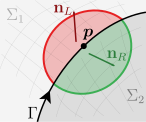
\includegraphics[width=5cm]{voisinage_courbe_singuliere.png}
%    \caption{Voisinage d'un point sur une courbe singulière.}
%\end{figure}



\section{Observations}%/Motivations}
[Objectif : justifier en quoi la construction intermédiaire d'une \guillemets{EdS partielle} (sous-ensemble de l'EdS qui contient l'EdB) permet de simplifier la construction d'un modèle \brep\ de l'EdB en évitant de construire des éléments de l'EdS qui sont trivialement exclues de l'EdB]
\par
définitions : 
\begin{itemize}
	\item \textit{zone d'influence}\footnote{\label{note_vocabulaire_notation}vocabulaire et notation à préciser \ldots} de $H \subseteq \Sigma$ sur l'EdB  (lieu des points de tangence entre $\EdB{\Sigma}{\rho}$ et $\sphere[H][\rho]$)
	\[ \influEdB{H}{\rho} := \EdB{\Sigma}{\rho} \cap \sphere[H][\rho] \]
	\item \textit{EdS propre}\footref{note_vocabulaire_notation} de $H \subseteq \Sigma$ 
	\[ \EdSpropre{H}{\rho} := \closure{ {\EdS{H}{\rho} \setminus \EdS{\boundary{H}}{\rho}} } \]
\end{itemize}
arguments :
\begin{enumerate}
	\item on sait décrire l'EdB simplement de manière \textit{implicite} (\cf \autoref{section:principe_huygens}) mais on cherche à en construire une représentation \textit{explicite}
	\item en revanche, on peut décrire explicitement l'EdS de chaque carreau ($\to$ introduire système définissant l'EdS à 2 paramètres)
	\item il est plus commode de voir l'EdS d'un carreau comme (un sous-ensemble de) la réunion de 10 nouveaux carreaux (intérieur $\to 2$ , bords $\to 4$ et ``coins'' $\to 4$)
	\item si on procède ainsi pour chaque carreau qui décrit l'interface, on construit beaucoup de nouveaux carreaux qui sont redondants, voire même trivialement exclus de l'EdB
%	\item la zone d'influence sur l'EdB d'une courbe singulière concave est vide (preuve?) (\ie cette courbe ne contribue pas à l'EdB et peut donc être ignorée)
%	\item la zone d'influence sur l'EdB d'une courbe singulière convexe $\Gamma$ est incluse dans la portion de son EdS qui est tangente aux EdS des deux nappes adhérentes à $\Gamma$ (preuve?), on appelle cette portion \textit{pseudo-EdS}\footref{note_vocabulaire_notation} de $\Gamma$ et on la note $\pseudoEdS{\Gamma}{\rho}$
	\item La zone d'influence sur l'EdB d'une courbe $\Gamma \subset \Sigma$ adhérentes aux nappes régulières $\Sigma_L$ et $\Sigma_R$ est incluse dans le lieu des points de tangence entre $\EdS{\Gamma}{\rho}$, $\EdS{\Sigma_L}{\rho}$ et $\EdS{\Sigma_R}{\rho}$ (on appelle ce lieu \textit{pseudo-EdS}\footref{note_vocabulaire_notation} de $\Gamma$ et on le note $\pseudoEdS{\Gamma}{\rho}$).
	\begin{proof}
		En posant\footnote{introduire ces notations dans la \autoref{section:principe_huygens}.}
		\[
			\implicitsphere(\bx, \p) := \normtwo{\bx - \p}^2 - \rho(\p)^2,
		\]
		et, pour $H \subseteq \Sigma$, 
		\[
			\implicitEdB{H}(\bx) := \min_{\p \in H} \implicitsphere(\bx, \p),
		\]
		on veut démontrer que 
		\[
			\influEdB{\Gamma}{\rho} \subseteq 
			\left\{
				\bx \in \complement{\Omega} \mid \implicitEdB{\Gamma}(\bx) = \implicitEdB{\Sigma_L}(\bx) = \implicitEdB{\Sigma_R}(\bx) = 0
			\right\}
			\subseteq \pseudoEdS{\Gamma}{\rho}.
		\]
		\par
		Puisque $\Gamma \subseteq \left( \closure{\Sigma_L} \cap \closure{\Sigma_R} \right)$, on a $\implicitEdB{\Gamma} \geq \implicitEdB{\Sigma_L}$ et $\implicitEdB{\Gamma} \geq \implicitEdB{\Sigma_R}$.\par
		Or, si $\bx \in \influEdB{\Gamma}{\rho}$ alors\footnote{car $\forall \bx \in \EdB{\Sigma}{\rho}, \implicitEdB{\Gamma}(\bx) \geq 0$ et $\forall \bx \in \sphere[\Gamma][\rho], \implicitEdB{\Gamma}(\bx) \leq 0$.} $\implicitEdB{\Gamma}(\bx) = 0$ et donc $\implicitEdB{\Sigma_L}(\bx) \leq 0$ et $\implicitEdB{\Sigma_R}(\bx) \leq 0$.\par
		Mais si $\implicitEdB{\Sigma_L} < 0$ ou $\implicitEdB{\Sigma_R} < 0$ alors\footnote{car $\forall H \subseteq \Sigma, \forall \bx \in \EdB{\Sigma}{\rho}, \implicitEdB{H}(\bx) \geq 0$.} $\bx \notin \EdB{\Sigma}{\rho}$ et donc $\bx \notin \influEdB{\Gamma}{\rho}$.\par
		Donc si $\bx \in \influEdB{\Gamma}{\rho}$ alors $\implicitEdB{\Sigma_L}(\bx) = 0$ et $\implicitEdB{\Sigma_R}(\bx) = 0$.
	\end{proof}
	
	\item Si $\Gamma$ est une courbe singulière concave de $\Sigma$ alors sa zone d'influence sur l'EdB est vide (\ie $\Gamma$ ne contribue pas à l'EdB et peut donc être ignorée).
	\begin{proof}
		On veut montrer que $\influEdB{\Gamma}{\rho} = \varnothing$ (piste : montrer que, pour $\bx \in \complement{\Omega}$, $\implicitEdB{\Gamma}(\bx) = 0 \Rightarrow \implicitEdB{\Sigma_L}(\bx) < 0$ ou $\implicitEdB{\Sigma_R}(\bx) < 0$)
	\end{proof}
	
	\item si toutes les courbes singulières adhérentes à un point singulier sont concaves alors la zone d'influence sur l'EdB de ce point est vide (preuve?) (\ie ce point ne contribue pas à l'EdB et peut donc être ignoré)
	\item si toutes les courbes singulières adhérentes à un point singulier $\p$ \textit{ne sont pas} concaves (ou bien que $\p$ n'est adhérent à aucune courbe singulière, \eg le sommet d'un cône) on dit que $\p$ est convexe et sa zone d'influence sur l'EdB est la portion de $\sphere[\p][\rho(\p)]$ qui est tangente aux EdS de toutes les courbes singulières adhérentes à $\p$ (preuve?), on appelle cette portion \textit{pseudo-EdS}\footref{note_vocabulaire_notation} de $\p$ et on la note $\pseudoEdS{\p}{\rho}$
	\item l'EdB est incluse dans la réunion
	\begin{itemize}
		\item des EdS propres des nappes régulières, qui sont elles-mêmes contenues dans la réunion des EdS propres des faces \brep
		\item des pseudo-EdS des courbes singulières convexes, qui sont elles-mêmes contenues dans la réunion des pseudo-EdS des arêtes \brep\ convexes
		\item des pseudo-EdS des points singuliers convexes, qui sont elles-mêmes contenues dans la réunion des pseudo-EdS des sommets \brep\ convexes
	\end{itemize}
	\item[$\Rightarrow$] on construit d'abord une telle réunion (que l'on appelle \textit{EdS partielle}\footref{note_vocabulaire_notation}) puis on en élimine les régions qui sont exclues de l'EdB (au passage on constitue les relations topologiques qui assurent la validité du modèle \brep)
\end{enumerate}



\setlength{\imagewidth}{50mm}%
\setlength{\imageheight}{\imagewidth}%
\begin{figure}
	\centering
%	\definecolor{colorContourEdSnappe0}{rgb}{1,0,0}
%	\definecolor{colorContourEdSnappe1}{rgb}{0,1,0}
%	\definecolor{colorContourEdSarete}{rgb}{0,0,1}
	\colorlet{colorContourEdSnappe0}{mycolor_2}
	\colorlet{colorContourEdSnappe1}{mycolor_3}
	\colorlet{colorContourEdSarete}{mycolor_1}
	\colorlet{colorInterieurEdSnappe0}{colorContourEdSnappe0}%!50!white}
	\colorlet{colorInterieurEdSnappe1}{colorContourEdSnappe1}%!50!white}
	\colorlet{colorInterieurarete}{colorContourEdSarete!30!white}
	\colorlet{colorPseudoEdSarete}{mycolor_4}%colorContourEdSarete!70!black}
	\begin{tikzpicture}[
		x = \imagewidth,
		y = \imageheight,
		styleEdS/.style = {
			thick, fill opacity=0.2
		},
		stylePseudoEdS/.style = {
			line width=1.1pt, colorPseudoEdSarete, line cap=round%, dash pattern=on 4pt off 3pt
		},
		styleNappe/.style = {
			draw=black, thick, line cap=round
		}
	]
		\begin{scope}
			%\clip (-1,-0.55) rectangle (1,0.8);
			\begin{scope}[blend group = overlay]
\draw[styleEdS, draw=colorContourEdSnappe0, fill=colorInterieurEdSnappe0] 
(1.0398871880695557, -0.05029176412270403) -- 
(1.0183167534800655, -0.0449025730216131) -- 
(0.9970249326809821, -0.03889063165462239) -- 
(0.9760087070839042, -0.03227375493086215) -- 
(0.9552635663797575, -0.025069985986572035) -- 
(0.9347833891410695, -0.017297348539330626) -- 
(0.9145603833626653, -0.008973612328943836) -- 
(0.8945850834066453, -0.00011607984793962633) -- 
(0.8748463978997224, 0.009258598781243438) -- 
(0.8553317017006214, 0.019134577567845562) -- 
(0.83602696412914, 0.029496929643137104) -- 
(0.816916905210558, 0.04033172390652845) -- 
(0.7979851716958212, 0.05162606350851576) -- 
(0.7792145250047978, 0.06336808792773979) -- 
(0.7605870339290941, 0.07554694172716503) -- 
(0.742084265838364, 0.08815271410883804) -- 
(0.7236874711762205, 0.10117635410812229) -- 
(0.7053777571313378, 0.11460956667949797) -- 
(0.68713624745879, 0.12844469504848804) -- 
(0.6689442264517612, 0.1426745945736954) -- 
(0.650783265984124, 0.1572925030243364) -- 
(0.6326353353336946, 0.1722919116818077) -- 
(0.6144828941409042, 0.18766644106904284) -- 
(0.5963089693558062, 0.20340972444626615) -- 
(0.5780972173844605, 0.21951530152848314) -- 
(0.5598319728767698, 0.2359765242139565) -- 
(0.5414982857190578, 0.2527864754915883) -- 
(0.5230819478253321, 0.26993790213828667) -- 
(0.5045695112809123, 0.28742316133741974) -- 
(0.4859482992996188, 0.3052341809521778) -- 
(0.4672064113277807, 0.3233624328735336) -- 
(0.4483327234793507, 0.34179891862769246) -- 
(0.4293168853280881, 0.36053416626560775) -- 
(0.4101493139242216, 0.37955823745850226) -- 
(0.3908211857508439, 0.3988607436785092) -- 
(0.3713244271940277, 0.4184308703424265) -- 
(0.35165170397301176, 0.4382574078293584) -- 
(0.33179640986407155, 0.4583287883406225) -- 
(0.3117526549541225, 0.4786331276446601) -- 
(0.291515253577205, 0.4991582708338544) -- 
(0.28440988145616547, 0.5063087863339162) -- 
(0.27710254029824977, 0.5132527729480235) -- 
(0.2695992307813853, 0.5199845283794992) -- 
(0.26190611450974904, 0.5264985246127) -- 
(0.25402950895395104, 0.5327894124525396) -- 
(0.24597588226322395, 0.5388520259171669) -- 
(0.23775184795387602, 0.5446813864801907) -- 
(0.2293641594783722, 0.5502727071589723) -- 
(0.22081970467950082, 0.5556213964456214) -- 
(0.2121255001341817, 0.5607230620774737) -- 
(0.20328868539155925, 0.5655735146439503) -- 
(0.19431651711011275, 0.5701687710268386) -- 
(0.18521636309859835, 0.5745050576711679) -- 
(0.17599569626571607, 0.5785788136839961) -- 
(0.1666620884834703, 0.5823866937585616) -- 
(0.1572232043692633, 0.5859255709213973) -- 
(0.147686794991827, 0.5891925391001548) -- 
(0.13806069150616307, 0.592184915510027) -- 
(0.1283527987227171, 0.59490024285681) -- 
(0.1185710886160675, 0.597336291354796) -- 
(0.10872359377846114, 0.5994910605578396) -- 
(0.09881840082356977, 0.6013627810020942) -- 
(0.0888636437458856, 0.6029499156590681) -- 
(0.07886749724120823, 0.6042511611978101) -- 
(0.06883816999370787, 0.6052654490551841) -- 
(0.058783897935078405, 0.6059919463133578) -- 
(0.048712937481315166, 0.606430056383782) -- 
(0.038633558752670744, 0.6065794194970995) -- 
(0.028554038782357544, 0.6064399129985829) -- 
(0.018482654719573693, 0.6060116514488569) -- 
(0.008427677032433106, 0.6052949865298223) -- 
(-0.0016026372836175917, 0.6042905067558604) -- 
(-0.011600051486318735, 0.602999036990554) -- 
(-0.02155635585048546, 0.601421637769322) -- 
(-0.031463374409710254, 0.5995596044285232) -- 
(-0.04131297167034209, 0.5974144660417463) -- 
(-0.051097059292231184, 0.5949879841641577) -- 
(-0.06080760273075139, 0.592282151385939) -- 
(-0.07043662783464624, 0.5892991896960018) -- 
(-0.07997622739428173, 0.5860415486573246) -- 
(-0.08941856763492664, 0.5825119033954085) -- 
(-0.09875589464973036, 0.5787131524015046) -- 
(-0.10798054076711328, 0.5746484151524166) -- 
(-0.11708493084734278, 0.5703210295488347) -- 
(-0.12606158850312335, 0.5657345491743005) -- 
(-0.1349031422390926, 0.5608927403770597) -- 
(-0.14360233150518156, 0.5557995791771925) -- 
(-0.15215201265886868, 0.550459248001567) -- 
(-0.16054516483143072, 0.5448761322492933) -- 
(-0.16877489569337395, 0.5390548166905) -- 
(-0.17683444711431084, 0.5330000817013907) -- 
(-0.18471720071263423, 0.526716899338671) -- 
(-0.19241668329043216, 0.5202104292565717) -- 
(-0.19992657214918022, 0.5134860144698171) -- 
(-0.2072407002818455, 0.5065491769660245) -- 
(-0.2143530614371397, 0.49940561317112975) -- 
(-0.22125781505176162, 0.4920611892715692) -- 
(-0.22794929104657935, 0.48452193639705643) -- 
(-0.23442199448281317, 0.4767940456679094) -- 
(-0.24067061007439672, 0.4688838631109964) -- 
(-0.24669000655280857, 0.4607978844484749) -- 
(-0.252475240880793, 0.45254274976360276) -- 
(-0.25802156231150697, 0.44412523804800214) -- 
(-0.2633244162897616, 0.43555226163485494) -- 
(-0.2683794481921539, 0.42683086052259867) -- 
(-0.2731825069030178, 0.4179681965937866) -- 
(-0.2777296482232569, 0.4089715477338585) -- 
(-0.2820171381092618, 0.39984830185465114) -- 
(-0.2860414557392498, 0.39060595082755645) -- 
(-0.28979929640451024, 0.38125208433131086) -- 
(-0.2932875742231817, 0.3717943836194658) -- 
(-0.2965034246743312, 0.3622406152126584) -- 
(-0.29944420695025553, 0.35259862452086255) -- 
(-0.3021075061250724, 0.3428763294008567) -- 
(-0.30449113513782133, 0.3330817136542001) -- 
(-0.30659313658844445, 0.3232228204710559) -- 
(-0.3084117843451744, 0.31330774582524457) -- 
(-0.30994558496200736, 0.30334463182595317) -- 
(-0.31119327890509796, 0.29334166003155904) -- 
(-0.31215384158707016, 0.2833070447310568) -- 
(-0.312826484208392, 0.2732490261986096) -- 
(-0.3132106544051267, 0.2631758639267602) -- 
(-0.3133060367025248, 0.2530958298438609) -- 
(-0.31311255277408784, 0.24301720152129108) -- 
(-0.3126303615058885, 0.23294825537604125) -- 
(-0.311859858866096, 0.22289725987424416) -- 
(-0.31080167757981286, 0.21287246874123647) -- 
(-0.3094566866094909, 0.20288211418372343) -- 
(-0.30782599044135184, 0.19293440012961588) -- 
(-0.3059109281784007, 0.18303749549108922) -- 
(-0.30371307244077433, 0.1731995274563957) -- 
(-0.3012342280743293, 0.16342857481594059) -- 
(-0.29847643066853036, 0.15373266132810265) -- 
(-0.2954419448848546, 0.14411974913024406) -- 
(-0.29213326259708616, 0.13459773220032423) -- 
(-0.28855310084502717, 0.12517442987448518) -- 
(-0.2847043996033055, 0.11585758042593017) -- 
(-0.2805903193671125, 0.10665483471037143) -- 
(-0.27621423855685184, 0.09757374988326305) -- 
(-0.2715797507438321, 0.08862178319397956) -- 
(-0.26669066169928013, 0.07980628586203543) -- 
(-0.26155098626909984, 0.07113449704037526) -- 
(-0.25616494507694093, 0.0626135378706904) -- 
(-0.2505369610582869, 0.0542504056356455) -- 
(-0.2446716558284075, 0.0460519680128164) -- 
(-0.23857384588715833, 0.03802495743505638) -- 
(-0.23224853866374337, 0.030175965561924676) -- 
(-0.2257009284046912, 0.022511437866715802) -- 
(-0.218936391908417, 0.015037668343533813) -- 
(-0.2119604841098781, 0.0077607943387599816) -- 
(-0.20477893351894494, 0.0006867915111568382) -- 
(-0.19739763751623587, -0.006178531075252337) -- 
(-0.18982265751027697, -0.0128295357214991) -- 
(-0.18206021395996608, -0.019260760723262417) -- 
(-0.17411668126642477, -0.025466924855938287) -- 
(-0.1659985825384379, -0.0314429317115007) -- 
(-0.13814675776047186, -0.051389728187050454) -- 
(-0.11010149732607256, -0.07084782564879044) -- 
(-0.08187628874232598, -0.08980691529833429) -- 
(-0.05348514223118164, -0.10825785303989452) -- 
(-0.024942488161001697, -0.1261927311153278) -- 
(0.0037369331581589837, -0.14360494415097552) -- 
(0.032538188799990014, -0.16048924853161478) -- 
(0.0614462769517472, -0.17684181400939064) -- 
(0.09044625611895998, -0.19266026647310083) -- 
(0.11952337865593937, -0.20794372084870297) -- 
(0.14866322725437772, -0.22269280317764836) -- 
(0.17785185281340019, -0.23690966102675073) -- 
(0.2070759119251168, -0.25059796152153513) -- 
(0.2363228020507566, -0.26376287646259583) -- 
(0.265580792345058, -0.2764110541778851) -- 
(0.29483914802179645, -0.2885505779777789) -- 
(0.32408824615147613, -0.30019091130722525) -- 
(0.35331968085209736, -0.3113428299218043) -- 
(0.38252635598214596, -0.32201834164250964) -- 
(0.4117025636751192, -0.33223059445727054) -- 
(0.4408440473670057, -0.3419937739254134) -- 
(0.46994804835801024, -0.3513229909948436) -- 
(0.49901333540890813, -0.3602341614525258) -- 
(0.5280402173876334, -0.36874387829068567) -- 
(0.5570305395358062, -0.37686927828051764) -- 
(0.58598766449683, -0.38462790400140734) -- 
(0.6149164398129897, -0.39203756247917254) -- 
(0.6438231541327407, -0.39911618144689354) -- 
(0.6727154848442609, -0.40588166406421605) -- 
(0.7016024402409139, -0.41235174272506525) -- 
(0.7304942996033684, -0.4185438323598505) -- 
(0.7594025547290846, -0.4244748834068749) -- 
(0.788339856433129, -0.4301612343982981) -- 
(0.8173199693690699, -0.43561846388665537) -- 
(0.8463577381635287, -0.44086124123470705) -- 
(0.8754690673157085, -0.44590317560849646) -- 
(0.9046709165817106, -0.4507566623537582) -- 
(0.9339813126454302, -0.4554327258016044) -- 
(0.9634193767817649, -0.4599408574440896) -- 
(0.9693155652265435, -0.4609052976013954) -- 
(0.9752369803674806, -0.4617002980555111) -- 
(0.9811787540119019, -0.4623252052100757) -- 
(0.9871360012297284, -0.462779505308097) -- 
(0.9931038243695415, -0.46306282485432837) -- 
(0.9990773170851042, -0.4631749309223312) -- 
(1.0050515683690329, -0.463115731345972) -- 
(1.0110216665902994, -0.4628852747951948) -- 
(1.0169827035322463, -0.46248375073600834) -- 
(1.022929778427797, -0.46191148927471937) -- 
(1.0288580019885372, -0.46116896088654163) -- 
(1.0347625004243635, -0.4602567760288024) -- 
(1.0406384194503882, -0.45917568463906483) -- 
(1.0464809282778087, -0.45792657551857996) -- 
(1.0522852235854594, -0.45651047560157293) -- 
(1.0580465334687832, -0.45492854911096664) -- 
(1.0637601213629715, -0.453182096601235) -- 
(1.0694212899370539, -0.4512725538891737) -- 
(1.0750253849557292, -0.4492014908734677) -- 
(1.0805677991057672, -0.4469706102440253) -- 
(1.0860439757838356, -0.4445817460821393) -- 
(1.0914494128426344, -0.4420368623526284) -- 
(1.0967796662922613, -0.439338051289196) -- 
(1.1020303539537641, -0.4364875316743353) -- 
(1.1071971590618763, -0.43348764701519416) -- 
(1.1122758338139729, -0.4303408636168996) -- 
(1.1172622028623307, -0.42704976855492677) -- 
(1.1221521667468217, -0.42361706754817735) -- 
(1.1269417052652146, -0.4200455827345184) -- 
(1.1316268807783172, -0.41633825035060845) -- 
(1.1362038414472417, -0.41249811831791966) -- 
(1.1406688244001288, -0.4085283437369402) -- 
(1.1450181588257307, -0.40443219029161614) -- 
(1.1492482689913066, -0.40021302556616906) -- 
(1.153355677182352, -0.3958743182764921) -- 
(1.1573370065617445, -0.3914196354184033) -- 
(1.161188983945953, -0.3868526393350996) -- 
(1.1649084424960312, -0.3821770847062224) -- 
(1.1684923243211818, -0.37739681546101034) -- 
(1.1719376829927497, -0.372515761618077) -- 
(1.1752416859665806, -0.36753793605441143) -- 
(1.1784016169117477, -0.3624674312062588) -- 
(1.18141487794374, -0.35730841570459176) -- 
(1.1842789917602683, -0.3520651309479401) -- 
(1.186991603677939, -0.346741887615396) -- 
(1.1895504835681168, -0.3413430621226607) -- 
(1.1919535276903879, -0.33587309302404755) -- 
(1.1941987604221163, -0.33033647736339883) -- 
(1.196284335882667, -0.32473776697691586) -- 
(1.1982085394509678, -0.31908156475094274) -- 
(1.1999697891751553, -0.3133725208377806) -- 
(1.2015666370731508, -0.30761532883264203) -- 
(1.202997770323094, -0.30181472191489017) -- 
(1.2042620123426586, -0.2959754689567343) -- 
(1.2053583237563583, -0.2901023706025812) -- 
(1.206285803250054, -0.2842002553222653) -- 
(1.207043688311952, -0.27827397544140275) -- 
(1.2076313558594922, -0.272328403152133) -- 
(1.2080483227516046, -0.2663684265075271) -- 
(1.2082942461859139, -0.2603989454029569) -- 
(1.2083689239805722, -0.25442486754772686) -- 
(1.2082722947404756, -0.24845110443028384) -- 
(1.2080044379077421, -0.24248256728031795) -- 
(1.2075655736963986, -0.2365241630310776) -- 
(1.206956062911335, -0.2305807902852156) -- 
(1.2061764066516745, -0.22465733528748522) -- 
(1.2052272458988051, -0.2187586679075953) -- 
(1.2041093609894056, -0.21288963763652835) -- 
(1.2028236709739044, -0.20705506959961203) -- 
(1.2013712328609003, -0.20125976058962325) -- 
(1.1997532407481573, -0.19550847512318478) -- 
(1.1979710248408986, -0.18980594152369779) -- 
(1.1960260503582012, -0.18415684803402882) -- 
(1.1939199163283891, -0.17856583896215006) -- 
(1.1916543542744191, -0.1730375108628982) -- 
(1.1892312267903393, -0.16757640875899452) -- 
(1.186652526009987, -0.1621870224044293) -- 
(1.1839203719691895, -0.15687378259328583) -- 
(1.1810370108628132, -0.15164105751703733) -- 
(1.1780048131980896, -0.14649314917331077) -- 
(1.1748262718457447, -0.14143428982907139) -- 
(1.1715039999905257, -0.13646863854113506) -- 
(1.1680407289828147, -0.13160027773686905) -- 
(1.164439306093095, -0.12683320985789287) -- 
(1.1607026921711152, -0.12217135406953673) -- 
(1.156833959211675, -0.11761854303876616) -- 
(1.1528362878290375, -0.11317851978321818) -- 
(1.1487129646420393, -0.10885493459394213) -- 
(1.1444673795720515, -0.10465134203437362) -- 
(1.1401030230560127, -0.1005711980180092) -- 
(1.1356234831768246, -0.09661785696718544) -- 
(1.1310324427134695, -0.09279456905529601) -- 
(1.1263336761132745, -0.08910447753471601) -- 
(1.1215310463888133, -0.08555061615262943) -- 
(1.1166285019419941, -0.0821359066568845) -- 
(1.1116300733179485, -0.07886315639392778) -- 
(1.1065398698913833, -0.0757350560007904) -- 
(1.1013620764881287, -0.07275417719302638) -- 
(1.0961009499446528, -0.06992297065041925) -- 
(1.090760815608376, -0.06724376400219671) -- 
(1.0853460637816557, -0.06471875991340899) -- 
(1.0798611461123757, -0.06235003427404442) -- 
(1.0743105719340957, -0.060139534492371444) -- 
(1.0686989045587796, -0.058089077893909054) -- 
(1.0630307575251439, -0.05620035022734317) -- 
(1.057310790805714, -0.05447490427861628) -- 
(1.0515437069757052, -0.052914158594330525) -- 
(1.0457342473468798, -0.05151939631551329) -- 
cycle; 
\coordinate (EdS0) at (0.5780972173844605, 0.21951530152848314);
\draw[styleEdS, draw=colorContourEdSnappe1, fill=colorInterieurEdSnappe1] 
(-0.15169069257764084, 0.5507561630088252) -- 
(-0.17504146443852367, 0.5360596714869722) -- 
(-0.1980509650850808, 0.521674771969309) -- 
(-0.22073415534445154, 0.5076006935349764) -- 
(-0.24310719678293558, 0.49383615486428445) -- 
(-0.2651874165214464, 0.48037937081071636) -- 
(-0.2869932690927314, 0.46722807665123334) -- 
(-0.3085442956789244, 0.4543795691229797) -- 
(-0.32986108091481187, 0.44183076319743253) -- 
(-0.35096520730549785, 0.42957826339985106) -- 
(-0.37187920718936585, 0.41761844835234146) -- 
(-0.3926265120789917, 0.40594756710319946) -- 
(-0.4132313991330905, 0.39456184570400504) -- 
(-0.4337189344495226, 0.3834576024096734) -- 
(-0.45411491281992367, 0.3726313698053583) -- 
(-0.47444579354746064, 0.3620800221069333) -- 
(-0.49473863189786793, 0.35180090583672363) -- 
(-0.5150210057287882, 0.34179197203978184) -- 
(-0.5353209368240557, 0.33205190817334773) -- 
(-0.5556668064512493, 0.3225802677669589) -- 
(-0.5760872646692548, 0.313377595905848) -- 
(-0.5966111329481912, 0.3044455485284712) -- 
(-0.6172672997411849, 0.29578700344381215) -- 
(-0.6380846087839275, 0.2874061608610278) -- 
(-0.6590917401143961, 0.27930863108194903) -- 
(-0.6803170841236117, 0.2715015068394799) -- 
(-0.7017886093907949, 0.2639934175814647) -- 
(-0.7235337256421194, 0.25679456281626867) -- 
(-0.7455791439158018, 0.24991672147641975) -- 
(-0.7679507369237274, 0.2433732341503716) -- 
(-0.790673403666179, 0.23717895501566963) -- 
(-0.8137709435620123, 0.23135017041918954) -- 
(-0.837265946664578, 0.22590448133181817) -- 
(-0.8611797078861451, 0.22086064739230282) -- 
(-0.8855321744698602, 0.21623839097508424) -- 
(-0.9103419371234759, 0.21205816068103941) -- 
(-0.9356262761334505, 0.20834085484647802) -- 
(-0.961401274258467, 0.20510750705228062) -- 
(-0.9876820080846747, 0.20237893711210087) -- 
(-1.0144828286234011, 0.20017537250377648) -- 
(-1.0212111055321056, 0.19966127297052094) -- 
(-1.0279217854342695, 0.19895361221776484) -- 
(-1.034609301063352, 0.19805297732998992) -- 
(-1.041268104370191, 0.1969601154855073) -- 
(-1.0478926711257381, 0.19567593333658903) -- 
(-1.0544775055040283, 0.194201496257298) -- 
(-1.0610171446415886, 0.19253802745963902) -- 
(-1.0675061631695015, 0.19068690697876728) -- 
(-1.0739391777143585, 0.18864967052809295) -- 
(-1.080310851364378, 0.18642800822523345) -- 
(-1.086615898096975, 0.18402376318987038) -- 
(-1.092849087164114, 0.18143893001467354) -- 
(-1.0990052474318048, 0.1786756531105611) -- 
(-1.105079271670143, 0.17573622492766872) -- 
(-1.1110661207903312, 0.17262308405350335) -- 
(-1.116960828025175, 0.1693388131898597) -- 
(-1.122758503049575, 0.16588613701017735) -- 
(-1.1284543360376047, 0.1622679198991166) -- 
(-1.134043601652803, 0.15848716357622827) -- 
(-1.1395216629683755, 0.15454700460568818) -- 
(-1.1448839753140478, 0.1504507117941632) -- 
(-1.1501260900463823, 0.146201683478967) -- 
(-1.1552436582394316, 0.14180344470875594) -- 
(-1.1602324342926624, 0.13725964431910287) -- 
(-1.1650882794531596, 0.13257405190537624) -- 
(-1.1698071652491915, 0.12775055469543542) -- 
(-1.1743851768322795, 0.12279315432473595) -- 
(-1.1788185162250082, 0.11770596351652171) -- 
(-1.1831035054718757, 0.11249320266985613) -- 
(-1.1872365896905732, 0.10715919635832517) -- 
(-1.1912143400211617, 0.1017083697423152) -- 
(-1.195033456470697, 0.09614524489784283) -- 
(-1.1986907706509484, 0.09047443706498239) -- 
(-1.2021832484069326, 0.08470065081900341) -- 
(-1.2055079923340877, 0.07882867616739407) -- 
(-1.2086622441819999, 0.07286338457600965) -- 
(-1.2116433871426804, 0.06680972492764123) -- 
(-1.2144489480215048, 0.06067271941635902) -- 
(-1.2170765992890076, 0.054457459381035425) -- 
(-1.2195241610118286, 0.048169101081504476) -- 
(-1.2217896026612163, 0.04181286142086249) -- 
(-1.223871044797579, 0.03539401361745781) -- 
(-1.225766760629692, 0.028917882830160894) -- 
(-1.2274751774472679, 0.022389841740544255) -- 
(-1.228994877925694, 0.01581530609563598) -- 
(-1.2303246013018665, 0.00919973021494658) -- 
(-1.2314632444201337, 0.002548602465495202) -- 
(-1.2324098626474882, -0.004132559291410428) -- 
(-1.2331636706572482, -0.010838212277863062) -- 
(-1.2337240430805723, -0.017562793397715527) -- 
(-1.2340905150252757, -0.024300723851797427) -- 
(-1.2342627824615098, -0.03104641376615843) -- 
(-1.2342407024739888, -0.03779426682950015) -- 
(-1.2340242933805552, -0.04453868493594776) -- 
(-1.2336137347169822, -0.05127407282931096) -- 
(-1.2330093670880287, -0.05799484274498075) -- 
(-1.2322116918848693, -0.06469541904561071) -- 
(-1.2312213708691342, -0.07137024284673765) -- 
(-1.2300392256239019, -0.0780137766285043) -- 
(-1.2286662368721049, -0.08462050882965623) -- 
(-1.2271035436629079, -0.09118495842000482) -- 
(-1.2253524424267392, -0.09770167944756064) -- 
(-1.2234143858997542, -0.10416526555656458) -- 
(-1.2212909819186275, -0.11057035447267138) -- 
(-1.2189839920866703, -0.11691163245156061) -- 
(-1.2164953303123824, -0.1231838386872879) -- 
(-1.213827061221648, -0.12938176967671738) -- 
(-1.2109813984448963, -0.13550028353641472) -- 
(-1.2079607027806447, -0.14153430426842012) -- 
(-1.2047674802369503, -0.14747882597136147) -- 
(-1.201404379952393, -0.15332891699341478) -- 
(-1.1978741919983158, -0.15907972402366605) -- 
(-1.1941798450641463, -0.1647264761184806) -- 
(-1.1903244040277179, -0.17026448865953914) -- 
(-1.1863110674126072, -0.17568916724025793) -- 
(-1.182143164734598, -0.18099601147736766) -- 
(-1.1778241537394727, -0.1861806187444887) -- 
(-1.1733576175344205, -0.1912386878246079) -- 
(-1.1687472616154468, -0.19616602247842244) -- 
(-1.1639969107932449, -0.20095853492559496) -- 
(-1.1591105060200841, -0.2056122492360284) -- 
(-1.154092101120346, -0.2101233046283487) -- 
(-1.1489458594274173, -0.21448795867285936) -- 
(-1.1436760503297374, -0.21870259039630863) -- 
(-1.1382870457288554, -0.22276370328589631) -- 
(-1.1327833164124483, -0.22666792819002524) -- 
(-1.1271694283452947, -0.23041202611339306) -- 
(-1.1214500388812925, -0.23399289090410488) -- 
(-1.1156298928996586, -0.23740755183057632) -- 
(-1.1097138188685158, -0.2406531760460909) -- 
(-1.1037067248391326, -0.2437270709389667) -- 
(-1.0976135943741416, -0.24662668636638074) -- 
(-1.0914394824131113, -0.24934961677000123) -- 
(-1.085189511078903, -0.2518936031716694) -- 
(-1.0788688654282916, -0.2542565350474768) -- 
(-1.072482789150376, -0.2564364520786833) -- 
(-1.0660365802163472, -0.25843154577802285) -- 
(-1.059535586484222, -0.26024016099004743) -- 
(-1.052985201262192, -0.261860797264266) -- 
(-1.0463908588342665, -0.26329211009993686) -- 
(-1.0397580299519174, -0.2645329120614833) -- 
(-1.0330922172954773, -0.26558217376360543) -- 
(-1.0263989509090414, -0.2664390247252709) -- 
(-1.0196837836126742, -0.26710275409187817) -- 
(-1.0129522863957163, -0.2675728112249897) -- 
(-1.0062100437950219, -0.2678488061591494) -- 
(-0.9994626492619538, -0.2679305099254024) -- 
(-0.9927157005219838, -0.2678178547412513) -- 
(-0.9618600215907757, -0.26718218439906705) -- 
(-0.9312831146272719, -0.2666713947766457) -- 
(-0.9009530059793759, -0.26625843546062694) -- 
(-0.8708379447198517, -0.2659148207309584) -- 
(-0.8409063796084735, -0.26561086314225923) -- 
(-0.8111270158339738, -0.2653158722753026) -- 
(-0.781468939498758, -0.2649983223125783) -- 
(-0.7519017969860202, -0.26462599327495656) -- 
(-0.7223960161469252, -0.26416609165852906) -- 
(-0.6929230564929207, -0.2635853567615401) -- 
(-0.6634556761362759, -0.26285015915721244) -- 
(-0.6339682039861398, -0.26192659754746617) -- 
(-0.6044368066058047, -0.2607805996498903) -- 
(-0.5748397401256944, -0.2593780318721067) -- 
(-0.5451575786645209, -0.25768482137646576) -- 
(-0.5153734118323504, -0.2556670928082199) -- 
(-0.48547300507696894, -0.25329132053369574) -- 
(-0.4554449178937359, -0.25052449579649216) -- 
(-0.4252805762499636, -0.24733430683318938) -- 
(-0.3949742969699929, -0.24368932877385877) -- 
(-0.36452326326741585, -0.23955921915536818) -- 
(-0.33392745206468954, -0.23491491415179303) -- 
(-0.30318951516469345, -0.2297288202133098) -- 
(-0.2723146176820055, -0.2239749957199047) -- 
(-0.241310238347933, -0.21762931749468523) -- 
(-0.21018593731769367, -0.2106696275580442) -- 
(-0.17895309788205088, -0.203075856293629) -- 
(-0.14762464898207767, -0.1948301191796247) -- 
(-0.1162147756228702, -0.18591678534310513) -- 
(-0.0847386241761405, -0.17632251734497642) -- 
(-0.05321200916732435, -0.16603628272319448) -- 
(-0.02165112749206638, -0.1550493388439899) -- 
(0.009927714853966221, -0.14335519347778738) -- 
(0.041508359462259836, -0.130949544186216) -- 
(0.07307503265108445, -0.11783020005372988) -- 
(0.1046125612256801, -0.1039969895135833) -- 
(0.13610656612738772, -0.08945165801084692) -- 
(0.16754363425536342, -0.07419775903601292) -- 
(0.19891146963183234, -0.058240541683307556) -- 
(0.2078176233741046, -0.053513397115755326) -- 
(0.21658463702996975, -0.04853294113247408) -- 
(0.22520530776875866, -0.04330326559216415) -- 
(0.23367255299267653, -0.03782866710811363) -- 
(0.2419794161557458, -0.032113643518173626) -- 
(0.25011907247918735, -0.026162890189410426) -- 
(0.25808483455854336, -0.01998129616047086) -- 
(0.2658701578579365, -0.013573940124830638) -- 
(0.27346864608695, -0.006946086258225556) -- 
(0.2808740564557121, -0.00010317989369318381) -- 
(0.28808030480386737, 0.006949156952220904) -- 
(0.29508147059921985, 0.014205130198417112) -- 
(0.3018718018019427, 0.021658778459561226) -- 
(0.3084457195903571, 0.029303977943858264) -- 
(0.3147978229443984, 0.03713444748425651) -- 
(0.32092289308300304, 0.04514375369894848) -- 
(0.3268158977517707, 0.053325316276928963) -- 
(0.33247199535738053, 0.06167241338426771) -- 
(0.3378865389453618, 0.070178187186655) -- 
(0.34305508001795404, 0.07883564948368263) -- 
(0.34797337218891744, 0.08763768745023151) -- 
(0.3526373746722923, 0.09657706948024913) -- 
(0.3570432556022406, 0.10564645112811495) -- 
(0.36118739518124277, 0.11483838114271346) -- 
(0.3650663886540617, 0.12414530758925614) -- 
(0.36867704910503296, 0.13355958405382418) -- 
(0.3720164100763803, 0.1430734759255331) -- 
(0.3750817280054082, 0.15267916675115878) -- 
(0.3778704844785657, 0.16236876465700348) -- 
(0.38038038830053345, 0.17213430883272657) -- 
(0.3826093773766308, 0.18196777607181205) -- 
(0.3845556204069979, 0.1918610873632996) -- 
(0.38621751839116114, 0.2018061145293642) -- 
(0.38759370594174447, 0.2117946869032897) -- 
(0.3886830524062495, 0.221818598042351) -- 
(0.38948466279597954, 0.23186961247008944) -- 
(0.38999787852134793, 0.2419394724424407) -- 
(0.39022227793296416, 0.2520199047321589) -- 
(0.3901576766680531, 0.2621026274259604) -- 
(0.38980412780192564, 0.2721793567288041) -- 
(0.3891619218043716, 0.2822418137697178) -- 
(0.3882315863010155, 0.2922817314035794) -- 
(0.38701388563982797, 0.30229086100326336) -- 
(0.3855098202631504, 0.3122609792365748) -- 
(0.3837206258857481, 0.3221838948223994) -- 
(0.3816477724795685, 0.3320514552605226) -- 
(0.3792929630660361, 0.34185555352958685) -- 
(0.3766581323168795, 0.35158813474768247) -- 
(0.37374544496463746, 0.36124120279010385) -- 
(0.3705572940241511, 0.3708068268588306) -- 
(0.3670962988265031, 0.38027714799833723) -- 
(0.3633653028670198, 0.3896443855523788) -- 
(0.3593673714691029, 0.398900843556447) -- 
(0.35510578926581204, 0.40803891706064477) -- 
(0.35058405750126476, 0.4170510983777851) -- 
(0.3458058911540741, 0.42592998325158) -- 
(0.34077521588518467, 0.434668276939853) -- 
(0.33549616481261524, 0.4432588002077763) -- 
(0.3299730751157592, 0.4516944952262091) -- 
(0.32421048447203105, 0.45996843137029075) -- 
(0.3182131273287865, 0.46807381091352634) -- 
(0.31198593101358096, 0.47600397461268296) -- 
(0.3055340116859604, 0.4837524071789122) -- 
(0.29886267013410983, 0.49131274263060226) -- 
(0.2919773874198163, 0.49867876952356016) -- 
(0.2848838203753203, 0.5058444360542305) -- 
(0.2775877969557575, 0.5128038550317544) -- 
(0.27009531145100973, 0.5195513087147872) -- 
(0.26241251956089684, 0.5260812535090974) -- 
(0.2545457333377575, 0.5323883245220917) -- 
(0.24650141600057368, 0.5384673399705187) -- 
(0.23828617662489873, 0.5443133054377355) -- 
(0.22990676471295257, 0.5499214179770362) -- 
(0.2213700646483436, 0.5552870700576722) -- 
(0.21268309003997596, 0.5604058533503213) -- 
(0.2038529779597865, 0.5652735623488971) -- 
(0.194886983079046, 0.569886197825722) -- 
(0.1857924717080448, 0.5742399701172248) -- 
(0.1765769157440554, 0.5783313022374652) -- 
(0.16724788653254827, 0.5821568328169241) -- 
(0.1578130486467014, 0.5857134188641493) -- 
(0.14828015359031646, 0.5889981383479833) -- 
(0.1386570334293139, 0.5920082925982559) -- 
(0.1289515943570395, 0.594741408522965) -- 
(0.11917181019866954, 0.597195240640128) -- 
(0.10932571586004947, 0.599367772922632) -- 
(0.0994214007263517, 0.6012572204545673) -- 
(0.08946700201597302, 0.6028620308976845) -- 
(0.0794706980951321, 0.6041808857667695) -- 
(0.06944070175866277, 0.6052127015128886) -- 
(0.059385253482519385, 0.6059566304136137) -- 
(0.049312614653541476, 0.6064120612694976) -- 
(0.03923106078203639, 0.6065786199062245) -- 
(0.02914887470276048, 0.6064561694820254) -- 
(0.019074339769881793, 0.6060448106001051) -- 
(0.009015733051514832, 0.6053448812259884) -- 
(-0.0010186814705782643, 0.6043569564098533) -- 
(-0.011020659690536047, 0.6030818478140791) -- 
(-0.020981984151616465, 0.6015206030463986) -- 
(-0.030894470797520404, 0.5996745047992016) -- 
(-0.04074997569627459, 0.5975450697956954) -- 
(-0.050540401731149445, 0.5951340475437916) -- 
(-0.06025770525311238, 0.5924434188987395) -- 
(-0.06989390268935552, 0.5894753944356885) -- 
(-0.07944107710246415, 0.5862324126335174) -- 
(-0.08889138469483893, 0.5827171378714212) -- 
(-0.09823706125302803, 0.5789324582399011) -- 
(-0.10747042852667375, 0.5748814831679595) -- 
(-0.11658390053683444, 0.570567540868444) -- 
(-0.12556998980849549, 0.5659941756036453) -- 
(-0.13442131352215392, 0.5611651447733902) -- 
(-0.14313059957941804, 0.5560844158280247) -- 
cycle; 
\coordinate (EdS1) at (-0.4337189344495226, 0.3834576024096734);
\end{scope}
\draw[styleEdS, draw=colorContourEdSarete, fill=colorInterieurarete] (0.03846156134313788, 0.25480769814250004) circle (0.3464951869522779);
\draw[stylePseudoEdS] (0.29657632742188633, 0.5040452822876815) arc (43.99759375651435:122.72148004933781:0.3588071986713943) node[above, pos=0.5, inner sep=2pt] {$\pseudoEdS{\crete}{\rho}$};
\path[decoration={text along path, raise={1ex}, text color=colorContourEdSarete, text={{$\implicitEdB{\crete}$} {$=$} {$0$}{}}, text align={center}}, decorate] (-0.21027863798930502, 0.0060674988100571925) arc (225:310:0.3517717634033278);
\draw[
    styleNappe,
    postaction={
        decoration={
            text along path, raise={1ex}, text={{$\Right{\nappe}$}{}}, text align=center, reverse path
        },
        decorate
    }
]
(1.0, -0.2548076981425002) .. controls (0.6394231211989716, -0.18750003123338313) and (0.33205293517056217, 0.00165690420180032) .. (0.03846156134313788, 0.25480769814250004) node[pos=0.35, above] (labelNappe0) {};
\node[colorContourEdSnappe0, inner sep=0.15\imagewidth, below] at (labelNappe0) {$\implicitEdB{\Right{\nappe}} < 0$};
\path[decoration={text along path, raise={1ex}, text color=colorContourEdSnappe0, text={{$\implicitEdB{\Right{\nappe}}$} {$=$} {$0$}{}}, text align={center}}, decorate] 
(0.291515253577205, 0.4991582708338544) -- 
(0.3117526549541225, 0.4786331276446601) -- 
(0.33179640986407155, 0.4583287883406225) -- 
(0.35165170397301176, 0.4382574078293584) -- 
(0.3713244271940277, 0.4184308703424265) -- 
(0.3908211857508439, 0.3988607436785092) -- 
(0.4101493139242216, 0.37955823745850226) -- 
(0.4293168853280881, 0.36053416626560775) -- 
(0.4483327234793507, 0.34179891862769246) -- 
(0.4672064113277807, 0.3233624328735336) -- 
(0.4859482992996188, 0.3052341809521778) -- 
(0.5045695112809123, 0.28742316133741974) -- 
(0.5230819478253321, 0.26993790213828667) -- 
(0.5414982857190578, 0.2527864754915883) -- 
(0.5598319728767698, 0.2359765242139565) -- 
(0.5780972173844605, 0.21951530152848314) -- 
(0.5963089693558062, 0.20340972444626615) -- 
(0.6144828941409042, 0.18766644106904284) -- 
(0.6326353353336946, 0.1722919116818077) -- 
(0.650783265984124, 0.1572925030243364) -- 
(0.6689442264517612, 0.1426745945736954) -- 
(0.68713624745879, 0.12844469504848804) -- 
(0.7053777571313378, 0.11460956667949797) -- 
(0.7236874711762205, 0.10117635410812229) -- 
(0.742084265838364, 0.08815271410883804) -- 
(0.7605870339290941, 0.07554694172716503) -- 
(0.7792145250047978, 0.06336808792773979) -- 
(0.7979851716958212, 0.05162606350851576) -- 
(0.816916905210558, 0.04033172390652845) -- 
(0.83602696412914, 0.029496929643137104) -- 
(0.8553317017006214, 0.019134577567845562) -- 
(0.8748463978997224, 0.009258598781243438) -- 
(0.8945850834066453, -0.00011607984793962633) -- 
(0.9145603833626653, -0.008973612328943836) -- 
(0.9347833891410695, -0.017297348539330626) -- 
(0.9552635663797575, -0.025069985986572035) -- 
(0.9760087070839042, -0.03227375493086215) -- 
(0.9970249326809821, -0.03889063165462239) -- 
(1.0183167534800655, -0.0449025730216131) -- 
(1.0398871880695557, -0.05029176412270403);
\draw[
    styleNappe,
    postaction={
        decoration={
            text along path, raise={1ex}, text={{$\Left{\nappe}$}{}}, text align=center, reverse path
        },
        decorate
    }
]
(0.03846156134313788, 0.25480769814250004) .. controls (-0.28894796328001215, 0.06631655134905) and (-0.5865384951744124, -0.014423064681421358) .. (-0.9999999999999998, -0.0336538334545584) node[pos=0.65, above] (labelNappe1) {};
\node[colorContourEdSnappe1, inner sep=0.15\imagewidth, below] at (labelNappe1) {$\implicitEdB{\Left{\nappe}} < 0$};
\path[decoration={text along path, raise={1ex}, text color=colorContourEdSnappe1, text={{$\implicitEdB{\Left{\nappe}}$} {$=$} {$0$}{}}, text align={center}}, decorate] 
(-1.0144828286234011, 0.20017537250377648) -- 
(-0.9876820080846747, 0.20237893711210087) -- 
(-0.961401274258467, 0.20510750705228062) -- 
(-0.9356262761334505, 0.20834085484647802) -- 
(-0.9103419371234759, 0.21205816068103941) -- 
(-0.8855321744698602, 0.21623839097508424) -- 
(-0.8611797078861451, 0.22086064739230282) -- 
(-0.837265946664578, 0.22590448133181817) -- 
(-0.8137709435620123, 0.23135017041918954) -- 
(-0.790673403666179, 0.23717895501566963) -- 
(-0.7679507369237274, 0.2433732341503716) -- 
(-0.7455791439158018, 0.24991672147641975) -- 
(-0.7235337256421194, 0.25679456281626867) -- 
(-0.7017886093907949, 0.2639934175814647) -- 
(-0.6803170841236117, 0.2715015068394799) -- 
(-0.6590917401143961, 0.27930863108194903) -- 
(-0.6380846087839275, 0.2874061608610278) -- 
(-0.6172672997411849, 0.29578700344381215) -- 
(-0.5966111329481912, 0.3044455485284712) -- 
(-0.5760872646692548, 0.313377595905848) -- 
(-0.5556668064512493, 0.3225802677669589) -- 
(-0.5353209368240557, 0.33205190817334773) -- 
(-0.5150210057287882, 0.34179197203978184) -- 
(-0.49473863189786793, 0.35180090583672363) -- 
(-0.47444579354746064, 0.3620800221069333) -- 
(-0.45411491281992367, 0.3726313698053583) -- 
(-0.4337189344495226, 0.3834576024096734) -- 
(-0.4132313991330905, 0.39456184570400504) -- 
(-0.3926265120789917, 0.40594756710319946) -- 
(-0.37187920718936585, 0.41761844835234146) -- 
(-0.35096520730549785, 0.42957826339985106) -- 
(-0.32986108091481187, 0.44183076319743253) -- 
(-0.3085442956789244, 0.4543795691229797) -- 
(-0.2869932690927314, 0.46722807665123334) -- 
(-0.2651874165214464, 0.48037937081071636) -- 
(-0.24310719678293558, 0.49383615486428445) -- 
(-0.22073415534445154, 0.5076006935349764) -- 
(-0.1980509650850808, 0.521674771969309) -- 
(-0.17504146443852367, 0.5360596714869722) -- 
(-0.15169069257764084, 0.5507561630088252);
\coordinate (Gamma) at (0.03846156134313788, 0.25480769814250004);
\fill[black] (Gamma) circle (1.2pt);
\node[above] at (Gamma) {$\crete$};

			\node[colorContourEdSarete] at ([shift={(120:0.2\imagewidth)}]Gamma) {$\implicitEdB{\Gamma} < 0$};
		\end{scope}
	\end{tikzpicture}
	\caption{Vue en coupe \ldots}
\end{figure}







\section{Construction d'une EdS partielle}
\label{section:def_canal_surface}

[Objectif : donner les étapes de la construction d'une EdS partielle sous la forme d'un ensemble de carreaux restreints (paramétrisation + courbes de restriction du domaine paramétrique) avec des relations d'adjacences partielles)]




\subsection{Paramétrisation de l'EdS propre d'une face \brep}% carreau paramétrique restreint}
\label{section:parametrisation_eds_propre_face}
\begin{enumerate}
	\item paramétrisation $\eos$ de l'EdS propre d'un carreau non-restreint $\Sigma_0 \colon (\left[\lo{u},\hi{u}\right] \times \left[\lo{v},\hi{v}\right], \bs)$
	\begin{enumerate}
		\item rappeler système définissant une EdS propre à 2 paramètres
		\def\sysvspace{1.5ex}
		\begin{equation}
		    \left\{\begin{matrix}
		        \implicitsphere_{\rho}(\eos(u,v), \bs(u,v)) &= 0, \\[\sysvspace]
		        \frac{\partial }{\partial u}\implicitsphere_{\rho}(\eos(u,v), \bs(u,v)) &= 0, \\[\sysvspace]
		        \frac{\partial }{\partial v}\implicitsphere_{\rho}(\eos(u,v), \bs(u,v)) &= 0.
		    \end{matrix}\right.
		    \label{eq:sys_envelope_of_spheres}
		\end{equation}
		\item interprétation : intersection de cercles caractéristiques (voir figure \autoref{fig:EdS_propre_carreau}) $\to$ 2 points (\ie 2 nouveaux carreaux), on garde celui dans le sens de $+\unv$ (\ie $\EdSpropreplus{\Sigma_i}{\rho}$, l'autre ($\EdSpropremoins{\Sigma_i}{\rho}$) est trivialement exclu de l'EdB)
		\item paramétrisation à la Gelston \cite{gelston1995} : \\
		En considérant $\rho$ comme une fonction des paramètres $u$ et $v$, on peut réécrire le système \eqref{eq:sys_envelope_of_spheres} 
		\begin{equation}
		    \left\{\begin{matrix}
		        \normtwo{\eos - \bs}^2 - \rho^2 &= 0, \\
		        \dotprod{\left( \eos - \bs \right)}{\bsu} + \rho \rho_u &= 0, \\
		        \dotprod{\left( \eos - \bs \right)}{\bsv} + \rho \rho_v &= 0.
		    \end{matrix}\right.
		\end{equation}
		En effet $\dotprod{\left( \eos - \bs \right)}{\eos_u} = \dotprod{\left( \eos - \bs \right)}{\eos_v} = 0$ car le vecteur $\eos - \bs$ est orthogonal à $\sphere[\bs][\rho]$ et donc à $\EdSpropre{\Sigma_i}{\rho}$. 
		On cherche une paramétrisation de la forme
		\[
			\eos(u,v) = \bs(u,v) + \rho(u,v) \unv_{\envelope}(u,v),
		\]
		où $\unv_{\envelope}$ est la direction normale à $\EdSpropre{\Sigma_0}{\rho}$, qui vérifie
		\[
			\left\{\begin{matrix}
				\normtwo{\unv_{\envelope}} = 1,\\
				\dotprod{\unv_{\envelope}}{\bsu} = -\rho_u,\\
				\dotprod{\unv_{\envelope}}{\bsv} = -\rho_v.
			\end{matrix}\right.
		\]
		On décompose $\unv_{\envelope} = \mathrm{n}_u \bsu + \mathrm{n}_v \bsv + \mathrm{n}_n \unv$, où $\unv = \unitized{\crossprod{\bsu}{\bsv}}$.\\
		Puisque $\dotprod{\bsu}{\unv} = \dotprod{\bsv}{\unv} = 0$, on a 
		\[
			\transpose{\jacobian{\bs}} \unv_{\envelope} = \fff_{\bs} \colvec{\mathrm{n}_u \\ \mathrm{n}_v} = -\colvec{\rho_u \\ \rho_v}.
		\]
		Si on pose $\vrm{t} = \jacobian{\bs} \colvec{\mathrm{n}_u \\ \mathrm{n}_v}$ (on a alors $\unv_{\envelope} = \vrm{t} + \mathrm{n}_n \unv$), on a
		\[
			\vrm{t} = - \jacobian{\bs} \inverse{ \left(\fff_{\bs}\right) } \colvec{\rho_u \\ \rho_v},
		\]
		soit
		\[
			\vrm{t} = \frac{
				\left( \rho_v I_{1,2} - \rho_u I_{2,2} \right) \bsu + 
				\left( \rho_u I_{1,2} - \rho_v I_{1,1} \right) \bsv
			}{
				\determinant{\fff_{\bs}}
			}.
		\]
		Si $\normtwo{\vrm{t}} \leq 1$ alors on a $\unv_{\envelope}^{\pm} = \vrm{t} \pm \sqrt{1 - \normtwo{\vrm{t}}^2} \unv$.
				
		\item différence avec le simple transport suivant la normale (ordre 2 en temps) \cite{jiao2001}
	\end{enumerate}
	\item conservation du domaine paramétrique (pas de re-paramétrisation) $\Rightarrow$ coordonnées $(x,y,z)$ des courbes de restriction données directement par la nouvelle paramétrisation
\end{enumerate}


%\begin{figure}[!htp]
%	\centering
%	\begin{tikzpicture}[
%		scale=1.5,
%		point/.style = {circle, scale=0.27, fill=black},
%		vector/.style = {-latex', thick},
%		label/.style = {inner sep=2pt},
%		txt/.style = {font=\small}]
%		\node[anchor=north west, inner sep=0] at (0,0) {\includegraphics[width=12cm]%width=scale*80mm
%		{figures/2pEoS_no_isouv}};
%		\coordinate (s) at (40.632mm,-21.936mm);
%		%
%		\coordinate (pp) at (38.4mm,-9.56mm);
%		\node [anchor=north, txt, xshift=0pt, label] at (pp) {$\eos^+$};
%		\coordinate (pm) at (38.76mm,-32.4mm);
%		\node [anchor=south, txt, xshift=3pt, yshift=2pt, label] at (pm) {$\eos^-$};
%		%
%		\coordinate (svmax) at (8.416mm,-34.856mm);
%		\coordinate (sv) at ($(s)!-0.55!(svmax)$);
%		\draw [vector, blue] (s) -- (sv) node [above, label, txt] {$\bs_v$};
%		\coordinate (sumax) at (60.872mm,-35.28mm);
%		\coordinate (su) at ($(s)!0.65!(sumax)$);
%		\draw [vector, red] (s) -- (su) node [right, label, txt] {$\bs_u$};
%		%
%		\coordinate (nmax) at (40.472mm,-6.176mm);
%		\coordinate (n) at ($(s)!0.4!(nmax)$);
%		\draw [vector] (s) -- (n) node [right, label, txt, black] {$\unv$};
%		%
%		\coordinate (qp) at ($(s)!1.6!(pp)$);
%		\node [anchor=west, label, txt, xshift=0pt] at (qp) {$\unv_{\envelope}^+$};
%		\draw [dotted, thick, shorten >= 14pt] (s) -- (pp);
%		\draw [vector] (pp) -- (qp);
%		%
%		\coordinate (qm) at ($(s)!1.6!(pm)$);
%		\node [anchor=east, label, txt, xshift=0pt]	at (qm) {$\unv_{\envelope}^-$};
%		\draw [dotted, thick, shorten <= 0pt, shorten >= 14pt] (s) -- (pm);
%		\draw [vector] (pm) -- (qm);
%		%
%		\node [point] at (s) {};
%		\node [point] at (pp) {};
%		\node [point] at (pm) {};
%		%
%%		\node [anchor=north, txt, inner sep=3pt] at (s) {$\bs(u,\!v)$};
%		%\node [anchor=west, txt, inner sep=4pt] at (s) {$\bs(u,\!v)$};
%		\node [anchor=east, txt, inner sep=2pt] at (s) {$\bs(u,v)$};
%		\node [txt, label] at (5.49mm,-15mm) {$\Sigma$};
%	\end{tikzpicture}
%	\caption{Paramétrisation de l'EdS propre d'un carreau paramétrique.}
%	\label{fig:EdS_propre_carreau}
%\end{figure}

\begin{figure}%[!htp]
	\centering
	\setlength{\imagewidth}{120mm}%
	\setlength{\imageheight}{0.625\imagewidth}%
	\DTLsetseparator{,}%
	\DTLloaddb[noheader,keys={x,y}]{dbsurfpoint}{figures/data/EdS_propre_carreau/surface_point.dat}%
	\DTLloaddb[noheader,keys={x,y}]{dbsurfvectors}{figures/data/EdS_propre_carreau/surface_vectors.dat}%
	\DTLloaddb[noheader,keys={x,y}]{dbEdSpoints}{figures/data/EdS_propre_carreau/envelope_points.dat}%
	\DTLloaddb[noheader,keys={x,y}]{dbEdSnormals}{figures/data/EdS_propre_carreau/envelope_normals.dat}%
	\begin{tikzpicture}[
		x = \imagewidth,
		y = \imageheight,
		point/.style = {circle, scale=0.27, fill=black},
		vector/.style = {-latex', thick},
		label/.style = {inner sep=2pt},
		txt/.style = {font=\small}
	]
		\node[anchor=south west, inner sep=0] at (0,0) {\includegraphics[width=\imagewidth]{figures/images/EdS_propre_carreau/EdS_propre_carreau.png}};
		%\drawGrid{10}{10}{black, thin, dotted}
		\DTLassign{dbsurfpoint}{1}{\spx=x, \spy=y}
		\coordinate (s) at (\spx, \spy);
		%
		\DTLassign{dbEdSpoints}{1}{\eppx=x, \eppy=y}
		\DTLassign{dbEdSpoints}{2}{\empx=x, \empy=y}
		\coordinate (ep) at (\eppx, \eppy);
		\coordinate (em) at (\empx, \empy);
		\node [anchor=north, txt, xshift=0pt, label] at (ep) {$\eos^+$};
		\node [anchor=south, txt, xshift=3pt, yshift=2pt, label] at (em) {$\eos^-$};
		%
		\DTLassign{dbsurfvectors}{1}{\sux=x, \suy=y}
		\coordinate (su) at (\sux, \suy);
		\draw [vector, red] (s) -- (su) node [below, xshift=-1pt, label, txt] {$\bsu$};
		%
		\DTLassign{dbsurfvectors}{2}{\svx=x, \svy=y}
		\coordinate (sv) at (\svx, \svy);
		\draw [vector, blue] (s) -- (sv) node [above, xshift=-5pt, label, txt] {$\bsv$};
		%
		\DTLassign{dbsurfvectors}{3}{\snx=x, \sny=y}
		\coordinate (sn) at (\snx, \sny);
		\draw [vector] (s) -- (sn) node [right, label, txt, black] {$\unv$};
		%
		\DTLassign{dbEdSnormals}{1}{\epnx=x, \epny=y}
		\coordinate (epn) at (\epnx, \epny);
		\node [anchor=west, label, txt, xshift=0pt] at (epn) {$\unv_{\envelope}^+$};
		\draw [dotted, thick, shorten >= 14pt] (s) -- (ep);
		\draw [vector] (ep) -- (epn);
		%
		\DTLassign{dbEdSnormals}{2}{\emnx=x, \emny=y}
		\coordinate (emn) at (\emnx, \emny);
		\node [anchor=west, label, txt, xshift=0pt] at (emn) {$\unv_{\envelope}^-$};
		\draw [dotted, thick, shorten <= 0pt, shorten >= 14pt] (s) -- (em);
		\draw [vector] (em) -- (emn);
		%
		\node [point] at (s) {};
		\node [point] at (ep) {};
		\node [point] at (em) {};
		%
		\node [anchor=east, txt, inner sep=2pt] at (s) {$\bs(u,v)$};
		\definecolor{colorSurfLabel}{rgb}{0.330, 0.413, 0.500}
		\node [txt, label, colorSurfLabel] at (0.1,0.68) {$\carreau$};
	\end{tikzpicture}
	\DTLgdeletedb{dbsurfpoint}%
	\DTLgdeletedb{dbsurfvectors}%
	\DTLgdeletedb{dbEdSpoints}%
	\DTLgdeletedb{dbEdSnormals}%
	\caption{Paramétrisation de l'EdS propre d'un carreau paramétrique.}
	\label{fig:EdS_propre_carreau}
\end{figure}

\begin{figure}
	\centering
	%\includegraphics[width=10cm]{EdS_propre_carreau_restreint.JPG}
	\setlength{\imagewidth}{80mm}%
\setlength{\imageheight}{0.75\imagewidth}%
\definecolor{colorEdS}{HTML}{81BD3E}%
%\definecolor{colorInterieurDomaineUV}{HTML}{ADD9F4}%
%\definecolor{colorBordDomaineUV}{HTML}{6BA2BF}%
%\colorlet{colorInterieurDomaineUV}{mycolor_5}%
%\definecolor{colorInterieurDomaineUV}{RGB}{235, 220, 178}
\definecolor{colorInterieurDomaineUV}{HTML}{FFEED5}%
\colorlet{colorBordDomaineUV}{colorInterieurDomaineUV!70!black}%
\definecolor{colorFace0}{HTML}{6BA2BF}%
\definecolor{colorFace1}{HTML}{C25D53}%
\begin{tikzpicture}[
	img/.style={anchor=south west, inner sep=0},
	axe/.style={-stealth, line width=0.5pt},
	axelabel/.style={font=\small},
	axeuvlabel/.style={axelabel, inner sep=0},
	map/.style={
		shorten >= 2pt,
		-{Classical TikZ Rightarrow[length=4pt,width=4pt]}
	}
]
	\begin{scope}[
		x=\imagewidth,
		y=\imageheight
	]
		\node[img] (3dscene) {\includegraphics[width=80mm]{EdS_propre_carreau_restreint/EdS_propre_carreau_restreint.png}};
		%\drawGrid{20}{20}{blue, thin, dotted}%%%
		\node[colorFace0] at (0.64, 0.31) {$\carreau$};
		\node[colorFace1] at (0.57, 0.455) {$\EdSpropreplus{\carreau}{\rho}$};
		\node[colorFace0!50!black] at (0.35, 0.55) {$\brepface$};
		\node[colorFace1, anchor=south, inner sep=0] at (0.355, 0.695) {$\EdSpropreplus{\brepface}{\rho}$};
		\node[colorEdS, anchor=west] at (0.81, 0.1) {$\EdS{\carreau}{\rho}$};
		\coordinate (destMap0) at (0.55, 0.3);
		\coordinate (destMap1) at (0.4, 0.93);%(0.375, 0.9);
	\end{scope}
	%
	\begin{scope}[
		x=0.3\imageheight,
		y=0.3\imageheight,
		shift={(-0.5\imageheight,0.5\imageheight)}
	]
		{\transparent{0.035}%
			\drawUVchecker{6}{black}
		}%
		\path[draw=colorBordDomaineUV, fill=colorInterieurDomaineUV, line width=0.6pt]
(0.5265310634108271, 0.438547589973437) .. controls (0.3310295488391929, 0.6935604776607408) and (-0.021382588776948222, 0.7376543228644009) .. (-0.10761414246666436, 0.6458722526584881)
.. controls (-0.21738265636518123, 0.5288877287485011) and (-0.17017248387614453, 0.367245125596702) .. (-0.2879469981322148, 0.19968851382281255)
.. controls (-0.40569858776829065, 0.03213190204887557) and (-0.6468263047931714, -0.04383071753181846) .. (-0.693539828033049, -0.2425873818597733)
.. controls (-0.7509242728775373, -0.48485275979627296) and (-0.41538197233103924, -0.7039845421685414) .. (-0.15341941399581885, -0.6891054816069568)
.. controls (0.1085262173182571, -0.6742682161592514) and (0.16478678736946484, -0.4840377550744662) .. (0.3373277172510478, -0.34364796735972497)
.. controls (0.5098686471326309, -0.20327907720189958) and (0.9385113528049314, -0.09879129235910938) .. (0.5265310634108271, 0.438547589973437)
-- cycle
(0.42885638368115414, 0.1734202847133243) .. controls (0.4481705327582044, -0.06518802075369291) and (0.280929641274987, -0.06594033280456221) .. (0.16421795586878063, -0.05212704764834414)
.. controls (0.047447004991011434, -0.03833466004908937) and (0.03296990893768833, 0.11674611021456661) .. (0.08180520084194194, 0.20877895110413416)
.. controls (0.13056009984453748, 0.3008326895506175) and (0.40950330245547123, 0.4120494877373048) .. (0.42885638368115414, 0.1734202847133243)
-- cycle
;
		\node[colorBordDomaineUV] at (-0.2, -0.25) {$\uvdomain$};
		\draw[axe] (-1,-1) -- ++ (2.05,0) node [below right, axeuvlabel] {$u$};
		\draw[axe] (-1,-1) -- ++ (0,2.05) node [above left, axeuvlabel] {$v$};
		%
		\node[inner sep=0.3] (uvcenter) at (0,0) {};
		\draw[map, colorFace0] (1.05, -0.45) to [bend right=20] node[below] {$\bs$} (destMap0);
		\draw[map, colorFace1] (1.05, 0.45) to [bend left=20] node[above] {$\eos$} (destMap1);
	\end{scope}
\end{tikzpicture}
	\caption{EdS propre d'un carreau paramétrique restreint.}
	\label{fig:EdS_propre_carreau_restreint}
\end{figure}



\subsection{Paramétrisation de la pseudo-EdS d'une arête \brep\ convexe}% arc paramétrique}
%\begin{enumerate}
%	\item détermination de la convexité de l'arête (signe de $\dotprod{\left(\crossprod{\unv_L}{\unv_R}\right)}{\vrm{t}}$, \cf \autoref{section:def_convexite_courbe_singuliere})
%	\item rappeler système définissant une EdS propre à 1 paramètre
%	\item notion de cercle caractéristique
%	\item paramétrisation générique $\eos(u,v) = \vit{o}(u) + r(u)\vrm{r}(u,v)$ de l'EdS propre
%	\item restriction à la portion entre les EdS propres des faces incidentes, paramétrisée sur le domaine $\uvdomain = \left[ \lo{u}, \hi{u} \right] \times \left[ \lo{v}, \hi{v} \right]$
%\end{enumerate}

\subsubsection{Paramétrisation de l'EdS propre d'un arc paramétrique}
\label{section:parametrisation_EdS_propre_courbe}

\begin{figure}
	\centering
	\setlength{\imagewidth}{120mm}%
	\setlength{\imageheight}{0.6857\imagewidth}%
	\definecolor{coloreos}{HTML}{64CF36}
	\definecolor{colorshpere}{HTML}{CD6E33}
	\begin{tikzpicture}[x=\imagewidth, y=\imageheight]
		\node[inner sep=0, anchor=south west] {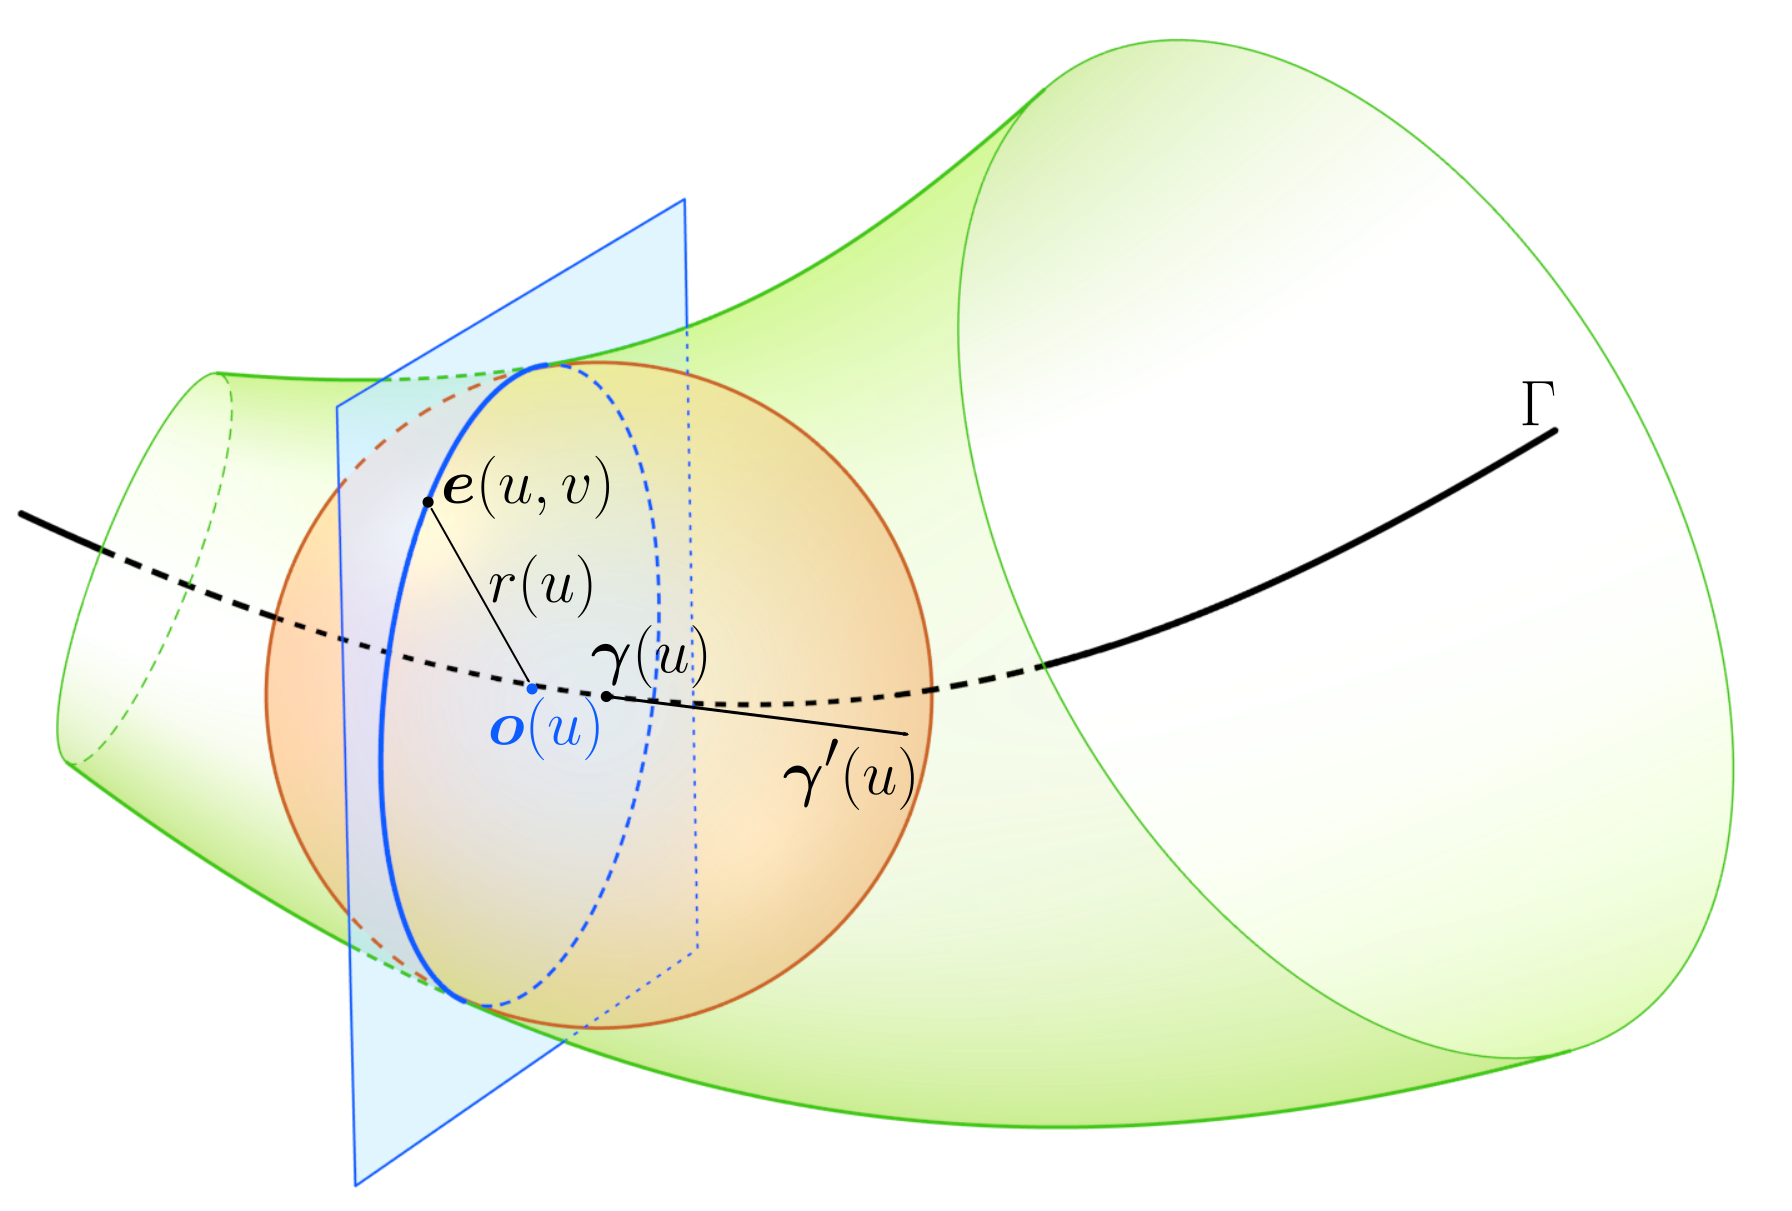
\includegraphics[width=\imagewidth]{figures/images/EdS_propre_courbe.png}};
		\node[coloreos] at (0.55,0.95) {$\EdSpropre{\Gamma}{\rho}$};
		\node[anchor=south west, colorshpere] at (0.46,0.62) {$\sphere[u]$};
	\end{tikzpicture}
	\caption{Paramétrisation de l'EdS propre d'un arc paramétrique.}
	\label{fig:parametrisation_EdS_propre_courbe}
\end{figure}
%%Soit $\bg : \wdomain \to \reals^3$ une paramétrisation du support géométrique $\Gamma$ de l'arête $\brepedge$. 
%%L'EdS propre de $\Gamma$ est le lieu des points $\bx \in \reals^3$ qui vérifient
%L'enveloppe $\Phi$ d'une famille de sphères à un paramètre centrées sur une courbe directrice $\Gamma$ est appelée \textit{surface canal} \cite{monge1850}. 
%Si la $\Gamma$ dispose d'une paramétrisation $\bg : \wdomain \to \reals^3$ alors cette surface est le lieu des points $\bx \in \reals^3$ qui vérifient
%\begin{equation}
%  \left\{
%    \begin{matrix}
%        \normtwo{\bx - \bg(u)}^2 - \rho(u)^2 &= 0 ,\\ 
%        \dotprod{\left(  \bx - \bg(u) \right)}{\bg'(u)} + \rho(u)\rho_u(u) &= 0.
%    \end{matrix}
%  \right.
%  \label{eq:sys_canal_surface}
%\end{equation}
Soit $\bg : \left[ \lo{u}, \hi{u} \right] \to \reals^3$ une paramétrisation du support géométrique $\Gamma$ de l'arête $\brepedge$. 
Si l'on considère $\rho$ comme une fonction du paramètre $u$ alors $\EdSpropre{\Gamma}{\rho}$ est le lieu des points $\bx \in \reals^3$ qui vérifient
\begin{equation}
  \left\{
    \begin{matrix}
        \normtwo{\bx - \bg(u)}^2 - \rho(u)^2 &= 0 ,\\ 
        \dotprod{\left(  \bx - \bg(u) \right)}{\bg'(u)} + \rho(u)\rho_u(u) &= 0.
    \end{matrix}
  \right.
  \label{eq:sys_canal_surface}
\end{equation}
A condition que $\rho_u^2 \leq \normtwo{\bg'}^2$, le système \eqref{eq:sys_canal_surface} définit une famille de \textit{cercles caractéristiques}, dont chacun est le lieu des points de tangence entre $\EdSpropre{\Gamma}{\rho}$ et une sphère de la famille $\sphere[\Gamma][\rho]$ (voir \autoref{fig:parametrisation_EdS_propre_courbe}).
\par
D'après \eqref{eq:sys_canal_surface}, le cercle caractéristique au point $\bg(u)$ est l'intersection de la sphère $\sphere[u] = \sphere[\bg(u)][\rho(\bg(u))]$ et d'un plan orthogonal à la tangente à $\Gamma$ en ce point (donnée par le vecteur $\bg'(u)$). 
Ce cercle est centré en
\begin{equation}
    \vit{o}(u) = \bg(u) - \frac{\rho(u)\rho_u(u)}{\normtwo{\bg'(u)}^2} \bg'(u),
    \label{eq:cercle_caracteristique_centre}
\end{equation}
et a pour rayon
\begin{equation}
    r(u) = \rho(u) \sqrt{1 - \frac{\rho_u(u)^2}{\normtwo{\bg'(u)}^2}}.
    \label{eq:cercle_caracteristique_rayon}
\end{equation}
\par
Voir $\EdSpropre{\Gamma}{\rho}$ comme une famille cercles caractéristiques permet d'en donner la paramétrisation suivante
\begin{equation}
    \eos(u,v) = \vit{o}(u) + r(u)\vrm{r}(u,v),
    \label{eq:parametrisation_EdS_propre_courbe}
\end{equation}
où $\vrm{r}$ vérifie
\begin{equation}
	\left\{
		\begin{matrix}
			\normtwo{\vrm{r}} = 1,\\ 
			\dotprod{\vrm{r}}{\bg'} = 0.
		\end{matrix}
	\right.
\end{equation}
De cette façon, les courbes iso-$u$ de $\eos$ sont les cercles caractéristiques.


\subsubsection{Paramétrisation de la pseudo-EdS}
\label{section:parametrisation_pseudo_EdS_arete}
\newcommand{\eosR}{\lo{\vit{\eos}}}
\newcommand{\eosL}{\hi{\vit{\eos}}}

\newcommand{\psiR}{\lo{\vit{\psi}}}
\newcommand{\psiL}{\hi{\vit{\psi}}}


\begin{figure}
    \centering
    \includegraphics[width=10cm]{pseudo-EdS_arete.JPG}
    \caption{Paramétrisation de $\pseudoEdS{\brepedge}{\rho}$}
    \label{fig:pseudo-EdS_arete}
\end{figure}






\subsection{Paramétrisation de la pseudo-EdS d'un sommet \brep\ convexe}
2 approches :

\subsubsection{Polygone sphérique découpé en quadrilatères}
\label{section:quadrangulation_polygone_spherique}
avantages/inconvénients :
\begin{itemize}
	\item[$-$] valable seulement si la vitesse normale est uniforme
	\item[$-$] génère plusieurs nouveaux carreaux de surface
	\item[$+$] les nouveaux carreaux sont rectangulaires ($\Rightarrow$ permet l'utilisation de quadratures simples (\cf \autoref{section:clenshaw_curtis_quadrature})
\end{itemize}


\subsubsection{Ajustement de carreau sphérique à un nuage de points}
\label{section:ajustement_carreau_spherique}

\def\s{\vit{s}}

%(\cf notes Huygens)
avantages/inconvénients :
\begin{itemize}
	\item[$-$] le nouveau carreau est restreint
	\item[$+$] valable également si la vitesse normale varie spatialement
	\item[$+$] génère un seul nouveau carreau de surface
\end{itemize}

Soit $\brepvertex$ un sommet \brep\ convexe dont le support géométrique est le point $\p$. 
On cherche à construire un carreau paramétrique restreint décrivant $\pseudoEdS{\p}{\rho}$ \ie la région de la sphère $\sphere[\p][\rho{\p}]$ délimitée par les arcs de cercles caractéristiques aux extrémités des arêtes \brep\ incidentes à $\p$. 
Afin de simplifier cette construction, on considère que $\p$ est situé à l'origine et que $\rho(\p) = 1$. 
(On appliquera la transformation adéquate en fin de construction pour se placer à nouveau dans le cas général.)
\par
Le problème consiste alors, étant donné un ensemble de points $S = \family{\s}{i}{1}{n}$ sur la sphère unité $\mathbb{S}^2$, à construire un carreau paramétrique décrivant une portion $R$ de $\mathbb{S}^2$ contenant $S$. 
On cherche également à minimiser l'aire de $R$ \ldots




\section{Construction d'un modèle \brep\ de l'EdB}

\subsection{Construction du graphe des intersections}
Conservation/création des intersections tangentielles, calcul des intersections transverses entre paire de carreaux non-restreints, segmentation des courbes d'intersection en segments quasi-disjoints (intersection de 3 carreaux non-restreints ou plus), \guillemets{clipping} par le domaine paramétrique de chaque carreau restreint
\par\bigskip
pour un carreau de surface, il s'agit d'un graphe planaire orienté dont un plongement dans $\reals^2$ est donné par la trace des courbes d'intersections dans son espace paramétrique

\begin{figure}
	\centering
	\plotCurvedDirectedGraph{/d/bandrieu/GitHub/FFTsurf/test/graph/graph_bezier_control_points.dat}{25mm}
	\caption{Plongement du graphe des intersections dans l'espace paramétrique d'un carreau de surface.}
\end{figure}


\subsection{Construction des faces, arêtes et sommets \brep}
pour chaque carreau : extraction des cycles du graphe d'intersection, caractérisations des contours (extérieurs/intérieurs), détermination des faces $\to$ insertion des contours dans la \brep\ $\to$ insertion des (co-)arêtes et sommets
\begin{figure}
	\centering
	\newcommand{\arc}{\mathcal{A}}%
\newcommand{\subin}{\ensuremath{_{\mathrm{in}}}}%
\newcommand{\subout}{\ensuremath{_{\mathrm{out}}}}%
\newcommand{\noeud}{\mathcal{N}}%
\newcommand{\cycle}{\mathcal{C}}%
\newcommand{\graph}{\mathcal{G}}%
\begin{tikzpicture}[%
	scale=0.5,
	>={Latex[length=4pt]},      % Arrow style
    start chain=going below,    % General flow is top-to-bottom
    node distance=6mm and 50mm, % Global setup of box spacing
    every join/.style={flow},   % Default linetype for connecting boxes
    ]
% ------------------------------------------------- 
% A few box styles 
% <on chain> *and* <on grid> reduce the need for manual relative
% positioning of nodes
\tikzset{
  base/.style={draw, on chain, on grid, align=center, minimum height=4ex, minimum width=5em},
  proc/.style={base, rectangle},
  test/.style={base, diamond, aspect=2},
  term/.style={proc, rounded corners=2ex},
  % coord node style is used for placing corners of connecting lines
  coord/.style={coordinate, on chain, on grid, node distance=6mm and 25mm},
  % -------------------------------------------------
  % Connector line styles for different parts of the diagram
  flow/.style={->, draw}
}
% -------------------------------------------------
\node [term, join] (start) {Début};
\node [proc, join] (p1) {Éliminer les branches pendantes de $\graph$};
\node [test, join] (t1) {$A = \emptyset$ ?};

\node [proc] (startarc) {Choisir un arc $\arc_*$ de $\graph$};

\node [proc, join] {Démarrer un nouveau cycle $\cycle$ à partir de $\arc_*$};
\node [proc, join] {$\arc \leftarrow \arc_*$ et\\ $\noeud \leftarrow \dest(\arc)$};


\node [test, join] (t2) {$\noeud = \orig(\arc_*)$?};

\node [proc] (maxangles) {Identifier $\hi{\alpha}\subin$, $\hi{\alpha}\subout$ et $\hi{\arc}\subout$};


\node [test, join] (t3) {$\hi{\alpha}\subin > \hi{\alpha}\subout$ ?};
\node [proc] (abortcycle) {Abandonner $\cycle$};

\node [term, left=of t1, text width=3em] (end) {Fin};
\node [proc, right=of t2] (completecycle) {Rajouter $\cycle$\\à la liste des cycles\\et l'extraire de $\graph$};
\node [proc, left=of t3] (appendcycle) {$\arc \leftarrow \hi{\arc}\subout$,\\ $\noeud \leftarrow \dest(\arc)$ et \\ajouter $\arc$ à $\cycle$};


\draw [flow] (t1.west) -- node[above] {oui} (end);
\draw [flow] (t1.south) -- node[left] {non} (startarc);

\draw [flow] (t2.east) -- node[above] {oui} (completecycle);
\draw [flow] (t2.south) -- node[left] {non} (maxangles);

\draw [flow] (t3.west) -- node[above] {oui} (appendcycle);
\draw [flow] (t3.south) -- node[left] {non} (abortcycle);


\draw [flow] (appendcycle.north) |- (t2);

\node [coord, left=of appendcycle] (c2)  {};
\draw [flow] (abortcycle.west) -| (c2) |- (p1);

\draw [flow] (completecycle.north) |- (p1);
% -------------------------------------------------
\end{tikzpicture}
	\caption{Organigramme de l'algorithme d'extraction des cycles d'un graphe orienté plongé dans $\reals^2$.}
\end{figure}


\begin{figure}
	\centering
	\setlength{\imagewidth}{60mm}%
\setlength{\imageheight}{\imagewidth}%
%
\colorlet{facecolor1}{mycolor_1}
\colorlet{facecolor2}{mycolor_2}
\colorlet{facecolor3}{mycolor_3}
%
\begin{tikzpicture}[
	x=0.5\imagewidth, 
	y=0.5\imageheight,
	halfedge/.style={
		line width=0.8pt, 
		line cap=round, 
		-{Triangle[left]}
	},
]
	\input{/d/bandrieu/GitHub/FFTsurf/test/graph/graph_faces_tikzcode.tex}
\end{tikzpicture}

	\caption{Faces du graphe}
\end{figure}

\chapter{Mise en \oe uvre numérique de l'algorithme de propagation}
\label{chap:methode_numerique}

Dans ce chapitre, on propose une mise en \oe uvre numérique de l'algorithme présenté au chapitre précédent. 
\begin{enumerate}
	\item choix de la discrétisation spatiale
	\begin{itemize}
		\item représentation des carreaux de surface
		\item représentation (et calcul) des courbes d'intersection entre carreaux
	\end{itemize}
	\item intégration temporelle
	\begin{itemize}
		\item intégration explicite du champ de vitesse 
		\item construction géométrique discrète de l'EdB suivant une méthode pseudo-spectrale (exacte aux points de collocation + interpolation)
	\end{itemize}
	\item considérations sur la stabilité numérique
\end{enumerate}



%\section{Discrétisation (pseudo-)spectrale en espace}
\section{Représentation des carreaux de surface}
\subsection{État de l'art}
\begin{enumerate}
	\item harmoniques sphériques \cite{rahimian2015}
	\item polynômes trigonométriques \cite{gueyffier2015}
	\item[$\Rightarrow$] limitations géométriques (régularité globale) et topologique (périodicité)
	\item modèle \brep\ permet une plus grande flexibilité
	\item polynômes algébriques (en produit tensoriel) adaptés aux carreaux de surface
	\item CAO : Bezier, NURBS $\to$ base des polynômes de Bernstein
	\begin{itemize}
		\item $B_n^N(x) = \binom{N}{n} \left( 1 - x \right)^{N-n} x^n$ pour $0 \leq n \leq N$.
		\item positivité : pour $0 \leq x \leq 1$, $B_n^N(x) \geq 0$
		\item partition de l'unité : $\sum_{n = 0}^N B_n^N = 1$
		\item[$\to$] propriétés intéressantes pour la conception géométrique
		\begin{itemize}
			\item coefficients = points de contrôle
			\item l'enveloppe convexe des points de contrôle englobe la courbe/surface de Bézier
		\end{itemize}
		\item inconvénients :
		\begin{itemize}
			\item points de contrôle pas \emph{sur} la courbe/surface $\Rightarrow$ pas exploitables comme marqueurs lagrangiens
			\item algorithme d'évaluation (de Casteljau) numériquement stable mais coûteux $\bigO{N^2}$
		\end{itemize}
	\end{itemize}
	\item motivation le choix des polynômes de Chebyshev
\end{enumerate}

%\subsection{Polynômes de Bernstein}
%Les polynômes de Bernstein sont définis par
%\begin{equation}
%	B_n^N(x) = \binom{N}{n} \left( 1 - x \right)^{N-n} x^n,
%	\label{eq:bernstein_poly}
%\end{equation}
%pour $0 \leq n \leq N$.
%Propriétés :
%\begin{itemize}
%	\item positivité : pour $0 \leq x \leq 1$, $B_n^N(x) \geq 0$
%	\item partition de l'unité : $\sum_{n = 0}^N B_n^N = 1$
%	\item dérivée : ${B_n^N}' = N \left( B_{n-1}^{N-1} - B_n^{N-1} \right)$
%\end{itemize}
%Avantages/inconvénients
%\begin{itemize}
%	\item[$+$] coefficients = points de contrôle dans l'espace physique, sens géométrique intuitif
%	\item[$+$] partition de l'unité sur $\berninterval$ $\Rightarrow$ propriété d'enveloppe convexe
%	\item[$\pm$] algorithme d'évaluation (de Casteljau) numériquement stable mais coûteux $\bigO{N^2}$
%	\item[$-$] points de contrôle pas \emph{sur} la courbe/surface $\Rightarrow$ pas exploitables comme marqueurs lagrangiens
%	\item[$-$] peu pratiques pour réduire/élever le degré des polynômes
%\end{itemize}


\subsection{Polynômes de Chebyshev univariés}
Les polynômes de Chebyshev sont très largement utilisés dans de nombreux domaines tels que l'analyse numérique.
L'objet des sections suivantes est de rappeler la définition de cette famille de polynômes et d'en présenter brièvement les propriétés remarquables qui seront exploitées dans cette thèse. 
Nombreux sont les ouvrages consacrés aux polynômes de Chebyshev \cite{mason2002, gil2007} ainsi qu'à leur usage dans les méthodes spectrales \cite{boyd2001, canuto2006}, aussi le lecteur est invité à s'y référer pour plus de détails.

\subsubsection{Définition et principales propriétés}
\begin{definition}
	Pour $n \in \mathbb{N}$, le polynôme de Chebyshev (de première espèce) $T_n$ est défini par%un polynome de degré $n$ défini par
	\begin{equation}
		T_n(\cos \theta) = n \cos \theta.
		\label{eq:chebyshev_trigo}
	\end{equation}
\end{definition}
%De la définition \eqref{eq:chebyshev_trigo} et de l'identité trigonométrique
De cette définition et de l'identité trigonométrique $\cos n\theta + \cos (n-2)\theta = 2\cos \theta \cos (n-1)\theta$, on peut déduire la relation de récurrence suivante, pour $-1 \leq x \leq 1$, 
\begin{align}[left = \empheqlbrace\,]
	T_0(x) &= 1, \nonumber\\
	T_1(x) &= x, \nonumber\\
	T_n(x) &= 2x T_{n-1}(x) - T_{n-2}(x) \text{,\ pour\ } n \geq 2.
	\label{eq:chebyshev_recurrence}
\end{align}
Le graphe des six premiers polynômes de Chebyshev est tracé sur la \autoref{fig:chebyshev_polynomials}.\par

\begin{figure}
	\centering
	%https://tex.stackexchange.com/questions/127375/replicate-the-fourier-transform-time-frequency-domains-correspondence-illustrati
\begin{tikzpicture}[%
		ax/.style={on layer=background, black, line width=0.5pt},
		grid/.style={on layer=background, black!25, line width=0.4pt},
		tickl/.style={font=\small},
		myax/.style={}
	]%
	\begin{axis}[
	width=12cm, height=9cm,
    set layers=standard,
    %domain=-1:1,
    xmin=-1, xmax=1,
    zmin=-1, zmax=1,
    samples y=1,
    view={40}{30},
    %hide axis,
    axis line style={draw=none},
    tick style={draw=none},
    grid = none,
    axis lines* = left,
    unit vector ratio*=4 3 1,
    %xtick=\empty, ytick=\empty, ztick=\empty,
    xtick={-1,-0.5,0,0.5,1},
    ytick={0,1,2,3,4,5},
    ztick={-1,0,1},
    %xlabel={$x$},
    %ylabel={$n$},
    %zlabel={$T_n(x)$},
    yticklabels=\empty,
    %zticklabels=\empty,
    no marks,
    samples=201,
    every tick label/.append style={font=\small},
    %tick align=outside,
%    cycle list/GnBu-9,%RdYlBu-6,%Spectral-6,
%	cycle multiindex* list={GnBu-9},%RdYlBu-6}%Spectral-6}
    clip=false
]
% x,z grid lines (at y=cst)
\foreach \y in {0,1,...,5}{%
	\foreach \x in {{-0.5},{0},{0.5},{1}}{
		\begingroup\edef\temp{\endgroup\noexpand\draw [grid] (axis cs:\x,\y,-1) -- ++ (axis direction cs:0,0,2);}\temp
	}
	\foreach \z in {{0},{1}}{
		\begingroup\edef\temp{\endgroup\noexpand\draw [grid] (axis cs:-1,\y,\z) -- ++ (axis direction cs:2,0,0,0);}\temp
	}
}
\pgfplotsinvokeforeach{0,1,...,5}{%
	\addplot3+[domain=-1:1]	({x},#1,{ cos(#1*acos(x)) });
%	\node[font=\footnotesize, anchor=west, inner sep=0] 
%		at (axis cs:1,#1,-0.3) {$n = #1$};
	\draw [ax] (axis cs:-1,#1,-1) -- ++ (axis direction cs:2,0,0); % x-axis
	\draw [ax] (axis cs:-1,#1,-1) -- ++ (axis direction cs:0,0,2); % z-axis
}%
% x,z ticks
\foreach \y in {0,1,...,5}{%
	\foreach \x in {{-1},{-0.5},{0},{0.5},{1}}{
		\begingroup\edef\temp{\endgroup\noexpand\draw [ax] (axis cs:\x,\y,-1) -- ++ (axis direction cs:0,0,0.2);}\temp
	}
	\foreach \z in {{-1},{0},{1}}{
		\begingroup\edef\temp{\endgroup\noexpand\draw [ax] (axis cs:-1,\y,\z) -- ++ (axis direction cs:0.05,0,0,0);}\temp
	}
}
% x, z tick labels and grid lines
%\pgfplotsinvokeforeach{-1,-0.5,0,0.5,1}{
%	\node[anchor=north, myax, tickl, xshift=-4pt] at (axis cs:#1,0,-1.1) {$#1$};
%%	\draw [grid] (axis cs:#1,0,-1) -- ++ (axis direction cs:0,5,0);
%}
%\pgfplotsinvokeforeach{-1,0,1}{
%	\node[anchor=east, myax, tickl] at (axis cs:-1,0,#1) {$#1$};
%%	\draw [grid] (axis cs:-1,0,#1) -- ++ (axis direction cs:0,5,0);
%}
% x,z labels
\node[anchor=north west, myax] at (axis cs:0,-1.1,-1) {$x$};
\node[anchor=south, rotate=90, myax, inner sep=7mm] at (axis cs:-1,0,0) {$T_n(x)$};
%
% y axis
\draw[ax, -latex] (axis cs:1.25,0,-1) -- ++ (axis direction cs:0,5.5,0) node[anchor=south west] {$n$};
\pgfplotsinvokeforeach{0,1,...,5}{%
	\draw[ax] (axis cs:1.25,#1,-1) -- ++ (axis direction cs:-0.05,0,0);
	\node[anchor=north west, myax, tickl] at (axis cs:1.25,#1,-1) {$#1$};
}
%\foreach \n in {0,1,...,5}{%
%	\node[font=\footnotesize, anchor=west, inner sep=0] 
%		at (axis cs:1,\n,-0.3) {$n = \n$};
%	\draw [ax] (axis cs:-1,\n,-1) -- ++ (axis direction cs:2,0,0); % x-axis
%	\draw [ax] (axis cs:-1,\n,-1) -- ++ (axis direction cs:0,0,2); % z-axis
%	\foreach \z in {-1,0,1}{%
%		\draw [ax] (axis cs:-1,\n,\z) -- ++ (axis direction cs:0.025,0,0);
%	}%
%	\foreach \x in {-1,-0.5,0,0.5,1}{%
%		\draw [ax] (axis cs:\x,\n,-1) -- ++ (axis direction cs:0,0,0.1);
%	}%
%}%
\end{axis}
\end{tikzpicture}
	\caption{Graphe des six premiers polynômes de Chebyshev.}% $(n=0,\ldots,5)$ sur l'intervalle $\chebinterval$.}
	\label{fig:chebyshev_polynomials}
\end{figure}

$T_n$ est un polynôme de degré $n$ %de coefficient dominant $2^{n-1}$ 
qui atteint ses extrema locaux sur $\chebinterval$ aux $n+1$ n\oe uds de Chebyshev-Gauss-Lobatto (CGL)%\footnote{Seuls les $n-1$ n\oe uds intérieurs sont réellement des extrema au sens où la dérivée s'y annule. A noter également que ces n\oe uds sont rangés en ordre décroissant.}
\begin{equation}
	x_k = \cos \frac{k \pi}{n},
	\label{eq:cgl_nodes}
\end{equation}
pour $0 \leq k \leq n$. 
Seuls les $n-1$ n\oe uds intérieurs sont réellement des extrema au sens où la dérivée s'y annule. 
À noter également que ces n\oe uds sont rangés en ordre décroissant.\par

\begin{figure}
	\centering
	\begin{tikzpicture} 
	\begin{axis}[%
		width=8cm, height=6cm,
		axis lines*=left,
		xmin=-1.0, xmax=1.0, ymin=-1.0, ymax=1.0,
		grid=major,
		clip marker paths=false,
		enlargelimits={abs=0.05},
		]%
		\addplot+[samples=200, domain=0:pi, no marks, s6] ({cos(deg(x))}, {cos(5*deg(x))});%
		% extrema
		\addplot+[samples=6, domain=0:pi, ycomb, dashed, mark=none, black] ({cos(deg(x))}, {cos(5*deg(x))});%
		\addplot+[samples=6, domain=0:pi, only marks, mark=*, black] ({cos(deg(x))}, {0});%
		% zeros
%		\pgfplotsinvokeforeach{0,...,4}{
%			\addplot+[mark=*, red] coordinates {(cos((2.0*#1+1.0)*180.0/10.0),0)};
%		}
	\end{axis} 
\end{tikzpicture}
%	\caption{N\oe uds de Chebyshev-Gauss-Lobatto pour $n = 6$ (extrema locaux du polynome $T_6$ sur l'intervalle $\chebinterval$).}
	\caption{N\oe uds de Chebyshev-Gauss-Lobatto (extrema locaux) du polynôme $T_5$.}% sur l'intervalle $\chebinterval$.}
	\label{fig:cgl_nodes}
\end{figure}

Comme illustré sur la \autoref{fig:cgl_nodes}, ces extrema sont alternativement des maxima puis des minima, tous égaux en valeur absolue
\begin{equation}
	T_n(x_k) = (-1)^{k}.
	\label{eq:chebyshev_equioscillation}
\end{equation}

Cette propriété d'\emph{équioscillation} a pour conséquence le théorème suivant.
\begin{theoreme}
	Le polynôme %$p_{N-1}$ 
	de degré $N-1$ qui donne la meilleure approximation uniforme (\ie en norme $L_\infty$) %de la fonction $x \mapsto x^N$ est $p_{N-1} : x \mapsto x^N - 2^{1 - N} T_n(x)$. 
du polynôme %$q : x \mapsto \sum_{n=0}^{N} a_n x^n$
$q = \sum_{n=0}^{N} a_n X^n$ 
sur l'intervalle $\chebinterval$ est
	\begin{equation}
		p_{N-1} = q - 2^{1-N} a_N T_N,
	\end{equation}
	et, pour tout $x \in \chebinterval$,
	%La meilleure approximation %uniforme (\ie en norme $L_\infty$) 
	%polynomiale de degré $N - 1$ en norme $L_\infty$ de la fonction $x \mapsto x^N$ sur $\chebinterval$ est la fonction $p_N : x \mapsto x^N - 2^{1 - N} T_n(x)$ et
	\begin{equation}
		%\norminf{q - p_{N-1}} = 2^{1-N} \left| a_N \right|.
		\left| q(x)-  p_{N-1}(x)\right| \leq 2^{1-N} \left| a_N \right|,
	\end{equation}
	l'égalité étant atteinte aux $N+1$ n\oe uds CGL de $T_N$.
\end{theoreme}
Ce théorème trouve une application immédiate dans l'économisation des séries \textit{(à développer\ldots)}.


\subsubsection{Approximation de fonctions}
%somme partielle, polynôme d'interpolation, erreurs de troncature et d'aliasing, DCT/FCT
Notons $\Ltwospace$ l'espace de Hilbert des fonctions de carré intégrable sur $\chebinterval$, muni du produit scalaire
\begin{equation}
	\scalprod{f}{g} =
	\int_{-1}^{1} \frac{f(x) g(x)}{\sqrt{1 - x^2}} \dx{x} .
	\label{eq:chebyshev_scalar_product}
\end{equation}

La famille des polynômes de Chebyshev est une base orthogonale et maximale de cet espace, et pour tous $m,n \in \mathbb{N}$,
\begin{equation}
	\scalprod{T_m}{T_n} =
	\frac{\pi}{2} \alpha_n \delta_{m,n},
	\label{eq:chebyshev_orthogonality}
\end{equation}
où $\delta_{\cdot,\cdot}$ représente le symbole de Kronecker, et
\begin{equation}
	\alpha_n = 
	1 + \delta_{0,n}.
%	\begin{cases}
%	 2 & \text{\ si\ } n = 0,   \\ 
%	 1 & \text{\ si\ } n > 0.\\ 
%	\end{cases}
\end{equation}

Toute fonction $f \in \Ltwospace$ peut alors être représentée par sa série de Chebyshev
\begin{equation}
	f = \sum_{n=0}^{\infty} \hat{f}_n T_n,
	\label{eq:chebyshev_series}
\end{equation}
dont les coefficients $\hat{f}_n$ sont obtenus en prenant le produit scalaire
\begin{align}
	\hat{f}_n 
	&= \frac{\scalprod{f}{T_n}}{\scalprod{T_n}{T_n}}, \nonumber \\
	&= \frac{2}{\pi \alpha_n} \int_{-1}^{1} \frac{f(x) T_n(x)}{\sqrt{1 - x^2}} \dx{x} .
	\label{eq:chebyshev_series_coeffs}
\end{align}

La somme partielle
\begin{equation}
	\truncseries{f}{N} = \sum_{n=0}^{N} \hat{f}_n T_n
	\label{chebyshev_truncated_series}
\end{equation}
est le projeté orthogonal de $f$ sur le sous-espace $\polyspace{N}$ de $\Ltwospace$ des polynômes de degré au plus $N$.
Il s'agit donc de l'élément de $\polyspace{N}$ le plus proche de $f$, au sens de la norme induite par le produit scalaire \eqref{eq:chebyshev_scalar_product}.\par
La somme partielle $\truncseries{f}{N}$ est également proche de la meilleure approximation uniforme de $f$ par un polynôme de degré N. 
En effet, si $f$ est continue sur $\chebinterval$, alors
\begin{equation}
	\norminf{f - \truncseries{f}{N}} 
	\leq 
	\left(1 + \lambda_N \right) 
	\min_{p \in \polyspace{N}} \norminf{f - p},
	\label{eq:chebyshev_near_minimax}
\end{equation}
où la constante de Lebesgue $\lambda_N = 1.27\ldots + \frac{4}{\pi^2} \log N + \bigO{N^{-1}}$ croît lentement avec $N$ ($\lambda_{500} \approx 3.8$).\par

Dans le contexte particulier de la résolution numérique d'équations aux dérivées partielles, %les séries de Chebyshev représentent un puissant outil pour l'approximation de fonctions possédant des dérivées continues, pour lesquelles la somme partielle $\truncseries{f}{N}$ converge très rapidement.
on s'intéresse à l'approximation de fonctions qui possèdent des dérivées continues.
Pour de telles fonctions, les séries de Chebyshev convergent très rapidement. 
En effet, à l'aide d'une intégration par parties répétée, on peut montrer que la relation \eqref{eq:chebyshev_series_coeffs} implique le théorème suivant.
\begin{theoreme}
	Si $f$ est $p-1$ fois dérivable presque partout sur \chebopeninterval\ et si $f^{(p-1)}$ est de variation bornée sur \chebinterval, alors 
	\begin{equation}
		\hat{f}_n = \bigO{n^{-p}}.
		\label{eq:chebyshev_convergence_coef_algebraic}
	\end{equation}
	En particulier, si $f \in \contdiff{\infty}\chebinterval$ alors la suite des coefficients $\hat{f}_n$ décroît plus rapidement que n'importe quelle puissance négative de $n$.\par
	En outre, si $f$ admet une extension analytique dans une région %\footnote{Il s'agit de la région bornée délimitée par l'ellipse de foyers $\pm 1$ et dont la somme des demi-axes vaut $r$.} 
	du plan complexe contenant le segment \chebinterval , alors il existe $r > 1$ tel que
	\begin{equation}
		\hat{f}_n = \bigO{r^{-n}}.
		\label{eq:chebyshev_convergence_coef_geometric}
	\end{equation}
\end{theoreme}
\par

Puisque $\left|T_n \right| \leq 1$ sur \chebinterval\ pour tout entier $n$, il s'ensuit que l'\textit{erreur de troncature} est bornée par la somme des valeurs absolues des coefficients négligés
\begin{equation}
	\norminf{f - \truncseries{f}{N}} \leq \sum_{n=N+1}^{\infty} 
	\left| \hat{f}_n \right|.
	\label{eq:chebyshev_truncation_error_bound}
\end{equation}

Or, si les coefficients $\hat{f}_n$ convergent avec une rapidité algébrique de la forme \eqref{eq:chebyshev_convergence_coef_algebraic}, alors\par
\begin{equation}
	\norminf{f - \truncseries{f}{N}} 
	= \bigO{N^{1-p}} 
	= \bigO{N \left| \hat{f}_N \right|}.
	\label{eq:chebyshev_truncation_error_estimator_algebraic}
\end{equation}

Si, en revanche, la convergence est géométrique (\ie de la forme \eqref{eq:chebyshev_convergence_coef_geometric}), alors 
\begin{equation}
	\norminf{f - \truncseries{f}{N}} 
	= \bigO{r^{-N}}
	= \bigO{\left| \hat{f}_N \right|}.
	\label{eq:chebyshev_truncation_error_estimator_geometric}
\end{equation}

Les règles empiriques \eqref{eq:chebyshev_truncation_error_estimator_algebraic} et \eqref{eq:chebyshev_truncation_error_estimator_geometric} permettent d'estimer efficacement l'erreur de troncature qui, en pratique, est inconnue. \textit{(dévélopper\ldots)}

\par\bigskip
\textit{Motivation pour interpolation\ldots}

%En pratique, l'intégrale \eqref{eq:chebyshev_series_coeffs} ne peut pas être calculée analytiquement  \ldots\\
Les polynômes de Chebyshev satisfont une seconde relation d'orthogonalité, dite \guillemets{discrète}, pour $0 \leq n \leq N$ et $m \geq n$,
\begin{equation}
	%\sum_{k=0}^{N}{''} T_m(x_k) T_n(x_k) = 
	\sum_{k=0}^{N} \frac{1}{\beta_k} T_m(x_k) T_n(x_k) = 
	\frac{N}{2} \beta_n \delta_{m,\pm n \bmod{2N}},
	\label{eq:chebyshev_discrete_orthogonality}
\end{equation}
où $\family{x}{k}{0}{N}$ sont les n\oe uds CGL de $T_N$ définis par l'équation \eqref{eq:cgl_nodes} et
\begin{equation}
	\beta_n = 
	1 + \delta_{0,n} + \delta_{N,n}.
%	\begin{cases}
%	 2 & \text{\ si\ } n = 0 \text{\ ou\ } N,   \\ 
%	 1 & \text{\ si\ } 0 < n < N.\\ 
%	\end{cases}
\end{equation}

%Le double prime dans l'équation \eqref{eq:chebyshev_discrete_orthogonality} signifie que les premier et dernier termes de la somme sont divisés par 2.
\par


Soit $\interpolant{f}{N}$ l'unique polynôme de $\polyspace{N}$ qui interpole $f$ aux $N+1$ n\oe uds CGL de $T_N$
\begin{equation}
	\interpolant{f}{N}(x_k) = f(x_k).
	\label{eq:chebyshev_interpolation_cgl}
\end{equation}

Ce polynôme peut s'exprimer dans la base de Chebyshev
\begin{equation}
	\interpolant{f}{N} = \sum_{n=0}^{N} \tilde{f}_n T_n.
	\label{eq:chebyshev_interpolant}
\end{equation}

En utilisant les relations \eqref{eq:chebyshev_interpolant}, \eqref{eq:chebyshev_interpolation_cgl} et \eqref{eq:chebyshev_discrete_orthogonality}, on peut alors déduire les coefficients $\tilde{f}_n$ à partir des valeurs de $f$ en ces n\oe uds
\begin{equation}
	%\tilde{f}_n = \frac{2}{\beta_n N} \sum_{k=0}^{N} {''} f(x_k) \cos \frac{n k \pi}{N}.
	\tilde{f}_n = \frac{2}{\beta_n N} \sum_{k=0}^{N} \frac{1}{\beta_k} f(x_k) \cos \frac{n k \pi}{N}.
	\label{eq:chebyshev_dct}
\end{equation}

L'équation \eqref{eq:chebyshev_dct} définit ainsi une transformation discrète [de l'espace \guillemets{physique} vers l'espace \guillemets{spectral}]\footnote{reformuler!}. 
Par ailleurs, des relations \eqref{eq:chebyshev_interpolation_cgl}, \eqref{eq:chebyshev_interpolant} et \eqref{eq:chebyshev_trigo}, on peut déduire la transformation inverse
\begin{equation}
	f(x_k) = \sum_{n=0}^{N} \tilde{f}_n \cos \frac{n k \pi}{N}.
	\label{eq:chebyshev_idct}
\end{equation}

Les équations \eqref{eq:chebyshev_dct} et \eqref{eq:chebyshev_idct} décrivent des transformations en cosinus discrètes (DCT), qui peuvent être effectuées efficacement à l'aide d'un algorithme de transformation de Fourier rapide (FFT) pour un coût asymptotique de $\bigO{N \log N}$ opérations.
\par
Les coefficients $\tilde{f}_n$ peuvent être reliés aux coefficients $\hat{f}_n$ par la relation
\begin{equation}
	\tilde{f}_n = \hat{f}_n + 
	\begin{cases}
		\displaystyle\sum_{j=1}^{\infty} \hat{f}_{2jN + n} & \text{\ si\ } n = 0 \text{\ ou\ } N,   \\[4ex]
		\displaystyle\sum_{j=1}^{\infty} \left( \hat{f}_{2jN - n} + \hat{f}_{2jN + n} \right) & \text{\ si\ } 0 < n < N. 
	\end{cases}
	\label{eq:chebyshev_aliasing}
\end{equation}

Cette relation met en évidence le phénomène d'\anglais{aliasing}, qui traduit le fait que les polynômes $T_n$ et $T_{\pm n \bmod{2N}}$ prennent les mêmes valeurs aux n\oe uds $\family{x}{k}{0}{N}$, comme illustré sur la \autoref{fig:aliasing_cgl}.
La différence entre le polynôme d'interpolation $\interpolant{f}{N}$ et la somme partielle $\truncseries{f}{N}$ est l'\textit{erreur d'aliasing}, qui est orthogonale à l'erreur de troncature\footnote{$\normtwo{\cdot}$ désigne ici la norme induite par le produit scalaire \eqref{eq:chebyshev_scalar_product}.}
\begin{equation}
	\normtwo{f - \interpolant{f}{N}}^2 = 
	\normtwo{f - \truncseries{f}{N}}^2 + 
	\normtwo{\interpolant{f}{N} - \truncseries{f}{N}}^2.
	\label{eq:chebyshev_aliasing_esrror}
\end{equation}

L'erreur d'approximation due à l'interpolation est donc toujours supérieure à l'erreur liée à la troncature de la série de Chebyshev.
Si $f$ est régulière, la suite des coefficients $\hat{f}_n$ converge rapidement vers zéro, si bien que l'erreur d'aliasing reste faible, à condition que le degré de troncature $N$ soit choisi suffisamment grand.
En outre, de la relation \eqref{eq:chebyshev_aliasing} on déduit que pour tout $x \in \chebinterval$,
\begin{equation}
	\left| f(x) - \interpolant{f}{N}(x) \right| \leq 2 \sum_{n>N} \left| \hat{f}_n \right|.
\end{equation}
L'erreur d'approximation due à l'interpolation est donc \textit{au pire} supérieure à l'erreur de troncature par un facteur 2.
L'erreur d'aliasing peut cependant devenir problématique lorsqu'elle est amplifiée par les non-linéarités présentes dans les équations que l'on sera amené à résoudre. 
Nous reviendrons sur ce point dans la \autoref{section:instabilités} lorsque nous aborderons \ldots

\begin{figure}
	\centering
	\begin{tikzpicture}
		\begin{axis}[%
			width=8cm, height=6cm,
			axis lines*=left,
			xmin=-1.0, xmax=1.0, ymin=-1.0, ymax=1.0,
			grid=major,
%			xtick = {-1,0,1},
%			ytick = {-1,0,1},
			clip marker paths=false,
			enlargelimits={abs=0.05},
			]%
			\addplot+[samples=200, domain=0:pi, no marks] ({cos(deg(x))}, {cos(3*deg(x))});% T_3
			\addplot+[samples=200, domain=0:pi, no marks] ({cos(deg(x))}, {cos(7*deg(x))});% T_7
			\addplot+[samples=500, domain=0:pi, no marks] ({cos(deg(x))}, {cos(13*deg(x))});% T_13
%			\addplot+[domain=-1:1, no marks, samples=200, black, dotted] {16*x^5 - 20*x^3 + 5*x};% T_5
			\addplot+[samples=6, domain=0:pi, ycomb, dashed, mark=*, black] ({cos(deg(x))}, {cos(3*deg(x))});% noeuds CGL de T_5
		\end{axis}
	\end{tikzpicture}
	\caption{Les polynômes $T_n (\protect\legenddash{mycolor_1})$, $T_{2N - n} (\protect\legenddash{mycolor_2})$ et $T_{2N + n} (\protect\legenddash{mycolor_3})$ sont indiscernables aux n\oe uds CGL de $T_N$ (ici, $n = 3$ et $N = 5$).}
	\label{fig:aliasing_cgl}
\end{figure}


\subsubsection{Évaluation d'une somme partielle}
Par la suite, nous serons amenés à évaluer à maintes reprises des sommes de la forme
\begin{equation}
	s_N = \sum_{n=0}^N \hat{s}_n T_n
	\label{eq:chebyshev_sum}
\end{equation}
en des points autres que les n\oe uds CGL.
Plutôt que de réécrire cette somme dans la base canonique de $\polyspace{N}$, il est intéressant de tirer parti de la relation \eqref{eq:chebyshev_recurrence}. 
En introduisant la suite récurrente
\begin{equation}
	b_n(x) = 
	\begin{cases}
	 0 & \text{\ si\ } n > N,   \\ 
	 \hat{s}_n - b_{n+2}(x) + 2x b_{n+1}(x) & \text{\ si\ } 0 \leq n \leq N,
	\end{cases}
\end{equation}
on obtient, pour $-1 \leq x \leq 1$,%
\def\px{}%{(x)}%
\begin{align*}
	s_N\px 
	&= \hat{s}_0 T_0\px + \hat{s}_1 T_1\px + \ldots + \hat{s}_{N-2} T_{N-2}\px + \hat{s}_{N-1} T_{N-1}\px + \hat{s}_N T_N\px, \\
	&= \hat{s}_0 T_0 \px
	+ \hat{s}_1 T_1 \px
	+ \ldots 
	+ \left(\hat{s}_{N-2} - b_{N}\px\right) T_{N-2} \px
	+ \left(\hat{s}_{N-1} - b_{N+1}\px + 2x b_{N}\px \right) T_{N-1}\px, \\
	&= \hat{s}_0 T_0 \px
	+ \hat{s}_1 T_1 \px
	+ \ldots 
	+ \left(\hat{s}_{N-3} - b_{N-1}\px\right) T_{N-3} \px
	+ b_{N-2}\px T_{N-2}\px, \\
	& \ldots\\
	&= \left( \hat{s}_0 - b_2\px \right) T_0\px + b_1\px T_1\px, \\
	&= \hat{s}_0 - b_2\px + b_1\px x,
\end{align*}
et enfin
\begin{equation}
	s_N(x) = b_0(x) - x b_1(x).
\end{equation}

L'exécution de cet algorithme de sommation --- proposé par Clenshaw \cite{clenshaw1955} --- requiert seulement $\bigO{N}$ opérations. %, ce qui le rend plus efficace que l'algorithme de Casteljau (dont la complexité est asymptotiquement quadratique). 
La sommation de Clenshaw est donc un moyen efficace et numériquement stable pour évaluer des séries de Chebyshev.

\subsubsection{Dérivation}
%% Dérivation
(versions matricielle (espace physique) et récursive (espace spectral)\par
quadrature de Clenshaw-Curtis)\par

En posant $x = \cos\theta$, il vient, d'après \eqref{eq:chebyshev_trigo},
\begin{equation}
	T_n'(x) := \dfdx{T_n(x)}{x} = \frac{n \sin n\theta}{\sin \theta}.
\end{equation}

Ainsi, de l'identité $2 \cos n \theta \sin \theta = \sin(n+1)\theta - \sin(n-1)\theta$, on peut déduire la relation 
\begin{equation}
	2 T_n = \frac{T'_{n+1}}{n+1} - \frac{T'_{n-1}}{n-1} ,
	\label{eq:chebyshev_relation_deriv_3termes}
\end{equation}
pour $n \geq 2$.
\\
Soit $f \in \contdiff{k}\chebinterval$.
On approche la dérivée $k$-ième $\deriv{f}{k}$ de $f$ par la dérivée $k$-ième du polynôme d'interpolation $\interpolant{f}{N}$
\begin{equation}
	\interpderiv{f}{N}{k} := \deriv{ \left( \interpolant{f}{N} \right) }{k}.
	\label{eq:chebyshev_def_interpderiv}
\end{equation}
En général, les opérations de dérivation et d'interpolation ne commutent pas, \ie
\begin{equation}
	\interpderiv{f}{N}{k} \neq \interpolant{ \left( \deriv{f}{k} \right) }{N}.
\end{equation}

Les valeurs aux n\oe uds CGL de cette dérivée peuvent être exprimées comme une combinaison linéaire des valeurs de $f$ en ces mêmes n\oe uds
\begin{equation}
	\colvec{ 
		\interpderiv{f}{N}{k}(x_0) \\ 
		\vdots \\
		\interpderiv{f}{N}{k}(x_N)
		}
	=
	{\left( \mathbf{D}_N \right)}^k
	\colvec{ 
		f(x_0) \\ 
		\vdots \\
		f(x_N)
		},
	\label{eq:chebyshev_diff_at_cgl}
\end{equation}
où $\mathbf{D}_N$ est la matrice de différentiation \cite{canuto2006}
\def\cvsp{2.5ex}
\begin{equation}
	\left( \mathbf{D}_N \right)_{i,j} =
	\begin{cases}
	 \dfrac{2N^2 + 1}{6} & \text{\ si\ } i = j = 0,   \\[\cvsp]
	 -\dfrac{2N^2 + 1}{6} & \text{\ si\ } i = j = N,   \\[\cvsp]
	 -\dfrac{x_i}{2 \sin^2 \frac{i \pi}{N}} & \text{\ si\ } 0 < i = j < N, \\[\cvsp]
	 -\dfrac{(-1)^{i+j} \beta_i}{2 \beta_j \sin\frac{(i+j)\pi}{2N} \sin\frac{(i-j)\pi}{2N}} & \text{\ si\ } i \neq j.
	\end{cases}
	\label{eq:chebyshev_diff_matrix}
\end{equation}

Alternativement, il est intéressant de construire explicitement le polynôme dérivé $\interpderiv{f}{N}{k}$ comme une somme de la forme 
\begin{equation}
	\interpderiv{f}{N}{k} = \sum_{n=0}^{N-k} \deriv{\tilde{f}}{k}_n T_n.
\end{equation} 
\textit{Développer motivation\ldots}

\par
La relation \eqref{eq:chebyshev_relation_deriv_3termes} implique que, pour tout $n \in \mathbb{N}$,
\begin{equation}
	2 (n + 1) \tilde{f}_{n+1} = \alpha_n \deriv{\tilde{f}}{1}_n - \deriv{\tilde{f}}{1}_{n+2}.
	\label{eq:chebyshev_prim_recurrence}
\end{equation}
Les coefficients $\deriv{\tilde{f}}{1}_n$ peuvent ainsi être calculés suivant la relation de récurrence
\begin{equation}
	\deriv{\tilde{f}}{1}_n = 
	\frac{1}{\alpha_n} \left( 2 (n + 1) \tilde{f}_{n+1} + \deriv{\tilde{f}}{1}_{n+2} \right).
	\label{eq:chebyshev_diff_recurrence}
\end{equation}
Plus généralement, les coefficients de Chebyshev de la dérivée $k$-ième vérifient
\begin{equation}
	\deriv{\tilde{f}}{k}_n = 
	\frac{1}{\alpha_n} \left( 2 (n + 1) \deriv{\tilde{f}}{k-1}_{n+1} + \deriv{\tilde{f}}{k}_{n+2} \right).
	\label{eq:chebyshev_diffp_recurrence}
\end{equation}

Cette méthode + FFT permet d'évaluer les dérivées aux n\oe uds CGL pour $\bigO{N + N \log N} = \bigO{N \log N}$, qui est asymptotiquement (au-delà de $N \approx 16$) plus efficace que le produit matrice-vecteur \eqref{eq:chebyshev_diff_at_cgl} ($\bigO{N^2}$).
\par
Toutefois, comme l'ont fait remarquer Wengle et Seinfeld \cite{wengle1978}, l'algorithme récursif \eqref{eq:chebyshev_diffp_recurrence} peut amplifier les erreurs d'arrondi commises sur les plus petits coefficients $\deriv{\hat{f}}{k-1}_{n}$ et ainsi compromettre la précision de \emph{tous} les coefficients $\deriv{\hat{f}}{k}_{n}$. 
Un moyen simple de remédier à ce problème consiste à mettre à zéro les coefficients $\deriv{\hat{f}}{k-1}_{n}$ inférieurs en valeur absolue à un seuil donné, choisi en fonction de la précision machine $\epsilon_M$. 
(Un seuil égal à $10 \epsilon_M$ semble être un bon choix \textit{(détailler\ldots)}.)

\par\bigskip

[Illustration de la qualité de l'approximation d'une fonction analytique (et ses dérivées)par le polynôme d'interpolation (et ses dérivées) (voir \autoref{fig:spectral_convergence_function} et \autoref{fig:spectral_convergence})]

\begin{figure}%[!htp]
\centering%
\begin{tikzpicture}%
\begin{axis}[%
	width=8cm, height=6cm,
	axis lines*=left,
	xmin=-1.0, xmax=1.0,
	ymin=-1.0, ymax=1.0,
	grid=major,
	ylabel={\small $\deriv{f}{k} \norminf{\deriv{f}{k}}^{-1}$},
%	xtick = {-1,0,1},
%	ytick = {-1,0,1},
	clip marker paths=false,
	%enlargelimits={abs=0.05},
	]%
	\pgfplotsinvokeforeach{1,...,3}{
		\addplot+[no marks] table[x index=0, y index=#1] {figures/data/Chebyshev/x_f0_f1_f2.dat};%
		%\addplot+[no marks] (x, {cos(3*x + #1)});
	}
\end{axis}%
\end{tikzpicture}%
\caption{Graphes de la fonction $f : x \mapsto e^{\sin 3 x^3}$ et ses dérivées $\deriv{f}{k}$ ($k = 0 (\protect\legenddash{mycolor_1}), \; 1 (\protect\legenddash{mycolor_2}), \; 2 (\protect\legenddash{mycolor_3})$).}%
\label{fig:spectral_convergence_function}%
\end{figure}

\begin{tikzpicture}
\begin{groupplot}[%
	group style={group size=2 by 1},
	ymode=log,
	width=7cm, height=6cm,
	xmin=0, xmax=80,
	ymin=1.0e-16, ymax=1.0e2,
	grid=major,
	axis x line*=bottom,
	xtick distance=20,
	%ytick align=outside,
	legend pos=south west,
	legend style={font=\small},
	]%
	%
	\nextgroupplot[%
		axis y line*=left,
		%yticklabel pos=right,
		xlabel={$N$},
		ylabel={$\left \| \interpolant{f}{N} - f \right \|_{\infty} / \left \| f \right \|_{\infty}$},
		]
		\addplot+ table[x index=0, y index=1] {figures/data/convergence_f.dat};%
		\addplot+ table[x index=0, y index=2] {figures/data/convergence_f.dat};%
		\addplot+ table[x index=0, y index=3] {figures/data/convergence_f.dat};%
		\addplot+[dashed, color=black, no marks, very thick][domain=25.5:54.5] 	{1e4*exp(-0.5*x)};%
		\legend{{$f$},{$f'$},{$f''$},{$e^{-0.5N}$}}%
		\coordinate (yl1) at (axis cs:80,1e2);%
		\coordinate (yl2) at (axis cs:80,1e-4);%
		\coordinate (yl3) at (axis cs:80,1e-10);%
		\coordinate (yl4) at (axis cs:80,1e-16);%
	%
	\nextgroupplot[%
		axis y line*=left,
		xlabel={$n$},
		ylabel={$\left | \tilde{f}_n \right |$},
		]
		\addplot+[only marks] table[x expr=\coordindex, y index=0] {figures/data/coeffs.dat};%
		\addplot+[only marks] table[x expr=\coordindex, y index=1] {figures/data/coeffs.dat};%
		\addplot+[only marks] table[x expr=\coordindex, y index=2] {figures/data/coeffs.dat};%
		\addplot+[dashed, color=black, no marks, very thick][domain=30.5:59.5] {1e6*exp(-0.5*x)};%
		\legend{{$f$},{$f'$},{$f''$},{$e^{-0.5n}$}}%
		\coordinate (yr1) at (axis cs:0,1e2);%
		\coordinate (yr2) at (axis cs:0,1e-4);%
		\coordinate (yr3) at (axis cs:0,1e-10);%
		\coordinate (yr4) at (axis cs:0,1e-16);%
\end{groupplot}
\end{tikzpicture}


\subsubsection{Intégration}
\label{section:clenshaw_curtis_quadrature}
La primitive de $\interpolant{f}{N}$ qui s'annule en $-1$
\begin{equation}
	\interpprim{f}{N} := x \mapsto \int_{-1}^{x} \interpolant{f}{N}(t) \dx{t}
\end{equation}

est un polynôme de degré $N+1$
\begin{equation}
	\interpprim{f}{N} = \sum_{n=0}^{N+1} \prim{\tilde{f}}{1}_n T_n.
\end{equation}

\eqref{eq:chebyshev_prim_recurrence} implique 
\begin{equation}
	\prim{\tilde{f}}{1}_n = \frac{\alpha_n \tilde{f}_{n-1} - \tilde{f}_{n+1}}{2n},
\end{equation}
pour $n \geq 1$ et, puisque $\interpprim{f}{N}(-1) = 0$, on a
\begin{equation}
	\prim{\tilde{f}}{1}_0 = - \sum_{n=1}^{N+1} (-1)^n \prim{\tilde{f}}{1}_n.
\end{equation}

\begin{equation}
	\int_{-1}^{x} f(t) \dx{t} 
	\approx \interpprim{f}{N}(x).
\end{equation}
En particulier,
\begin{equation}
	\int_{-1}^{1} f(t) \dx{t} 
	\approx 
	\interpprim{f}{N}(1)
	=
	\sum_{\mathclap{\substack{n = 0\\n \text{ pair}}}}^{N} \frac{2 \tilde{f}_n}{1 - n^2},
\end{equation}
et
\begin{equation}
	\left| \int_{-1}^{1} f(x) \dx{x} - \interpprim{f}{N}(1) \right|
	\approx
	\left|\frac{2 \tilde{f}_{N}}{1 - N^2}\right|.
\end{equation}

[$\to$ quadrature de Clenshaw-Curtis]








\subsection{Polynômes de Chebyshev bivariés}
\begin{itemize}
	\item Fonctions de base : polynômes de Chebyshev en produit tensoriel
	\[ \interpolant{f}{M,N}(u,v) = \sum_{m=0}^{M} \sum_{n=0}^{N} \tilde{f}_{m,n} T_m(u) T_n(v). \]
	\item généralisation des propriétés des polynômes univariés
	\item paramétrisation d'un carreau de surface
	\begin{equation}
		\bs(u,v) = \sum_{m=0}^{M} \sum_{n=0}^{N} \tilde{\bs}_{m,n} T_m(u) T_n(v).
	\end{equation}
	(les coefficients $\tilde{\bs}_{m,n}$ sont des vecteurs de $\reals^3$)
\end{itemize}

%\def\degru{6}
\def\degrv{5}
\def\uvsize{32mm}
\def\fracaxeoffset{0.1}
\def\fracduv{0.2}
\def\distanceaxe{1.7*\MajorTickLength}
\colorlet{uvbgcolor}{white!92!black}
\begin{figure}%
\centering%
\hspace*{\fill}%
\subbottom[Grille CGL $uv$.]{%
\begin{tikzpicture}[
	point/.style={circle, fill=black, scale=0.22},
	bigpoint/.style={circle, fill=black, scale=0.33},
	isouv/.style={dotted, line width=0.5pt},
	tick/.style={line width=0.5pt},
	axe/.style={-stealth, tick},
	label/.style={font=\small, inner sep=1.5pt},
	vector/.style={-latex', very thick},
	ticklabel/.style={label, inner sep=\MajorTickLength}]
%
\coordinate (uvnorth) at (0,{0.5*\parampatchimageheight});
\coordinate (uvsouth) at (0,{-0.5*\parampatchimageheight});
\node at (uvnorth) {};
\node at (uvsouth) {};
%
\foreach \j in {0,...,\degrv} {
	\foreach \i in {0,...,\degru} {
		\coordinate (uv\i\j) at (
			{0.5*cos(\i*pi/\degru r)*\uvsize},
			{0.5*cos(\j*pi/\degrv r)*\uvsize}
		);
	}
}
%
\draw[fill=uvbgcolor, semithick] 
(uv00) -- (uv\degru0) -- (uv\degru\degrv) -- (uv0\degrv) -- cycle;
%
\foreach \j in {0,...,\degrv} {
	\foreach \i in {0,...,\degru} {
		\node[point] at (uv\i\j) {};
	}
}
\foreach \i in {0,...,\degru} {\draw[isouv] (uv\i0) -- (uv\i\degrv);}
\foreach \j in {0,...,\degrv} {\draw[isouv] (uv0\j) -- (uv\degru\j);}
%
% Axes
\coordinate (o) at ({-0.5*\uvsize-\distanceaxe},{-0.5*\uvsize-\distanceaxe});
\draw[axe] (o) -- ++ ({(1.0+\fracaxeoffset)*\uvsize+\distanceaxe},0) node [label, anchor=west] {$u$};
\draw[axe] (o) -- ++ (0,{(1.0+\fracaxeoffset)*\uvsize+\distanceaxe}) node [label, anchor=south] {$v$};
% Ticks
\gettikzxy{(o)}{\ox}{\oy}
\foreach \i in {-1,0,1} {
	\draw[tick] ({0.5*\i*\uvsize},{\oy}) -- ({0.5*\i*\uvsize},{\oy+\MajorTickLength});
	\node[anchor=north, ticklabel] at ({0.5*\i*\uvsize},\oy) {$\i$};
}
\foreach \j in {-1,0,1} {
	\draw[tick] ({\ox},{0.5*\j*\uvsize}) -- (\ox+\MajorTickLength,{0.5*\j*\uvsize});
	\node[anchor=east, ticklabel] at (\ox,{0.5*\j*\uvsize}) {$\j$};
}
%
\def\i{4}
\def\j{3}
\node[label, fill=uvbgcolor, rectangle, rounded corners=1ex, label, anchor=north, inner sep=0.5pt, yshift=-1.5pt] at (uv\i\j) {$(u_i,v_j)$};
\draw[vector, red] (uv\i\j) -- ++ ({\fracduv*\uvsize},0);
\draw[vector, blue] (uv\i\j) -- ++ (0,{\fracduv*\uvsize});
\node[bigpoint] at (uv\i\j) {};
\end{tikzpicture}%
\label{subfig:cgl_grid_uv}%
}%
\hfill%
\subbottom[Grille CGL $xyz$.]{
\def\parampatchimagewidth{80mm}
\def\parampatchimageheight{0.75*\parampatchimagewidth}
\begin{tikzpicture}[
	x=\parampatchimagewidth,
	y=\parampatchimageheight,
	im/.style={anchor=south west, inner sep=0pt},
	bigpoint/.style={circle, fill=black, scale=0.33},
	axe/.style={-stealth, line width=0.5pt},
	label/.style={font=\small, inner sep=1.5pt},
	vector/.style={-latex', very thick}]
\coordinate (a) at (0,0);
{\transparent{\parampatchshadowtransparency}\node[im] (shadow) at (a) {\includegraphics[width=\parampatchimagewidth]{figures/parametric_patch_shadow}};}
% trièdre
\def\scaletriedre{0.85}
\coordinate (o) at (0.20309802889823914 ,  0.26374515891075134);
\coordinate (x) at (0.30103224515914917 ,  0.14841561019420624);
\coordinate (y) at (0.3310101628303528 ,  0.3642595410346985);
\coordinate (z) at (0.17395645380020142 ,  0.43496546149253845);
\draw[axe] (o) -- ($(o)!\scaletriedre!(x)$) node[label, anchor=west] {$x$};
\draw[axe] (o) -- ($(o)!\scaletriedre!(y)$) node[label, anchor=west] {$y$};
\draw[axe] (o) -- ($(o)!\scaletriedre!(z)$) node[label, anchor=south] {$z$};
%
\node[im] at (a) {\includegraphics[width=\parampatchimagewidth]{figures/parametric_patch_surface}};
\node[im] at (a) {\includegraphics[width=\parampatchimagewidth]{figures/parametric_patch_cgl_grid}};
\node[im] at (a) {\includegraphics[width=\parampatchimagewidth]{figures/parametric_patch_border}};
% vecteurs
\def\scalevectors{0.99}
\coordinate (s) at (0.5657749772071838, 0.4292657971382141);
\coordinate (u) at (0.6539148092269897, 0.5149791240692139);
\coordinate (v) at (0.506170392036438, 0.5304208993911743);
\coordinate (n) at (0.5878586769104004, 0.5399532318115234);
\draw[vector, red] (s) -- ($(s)!\scalevectors!(u)$) node[label, anchor=north west, xshift=-2pt] {$\bx_u$};
\draw[vector, blue] (s) -- ($(s)!\scalevectors!(v)$) node[label, anchor=east, yshift=-1pt] {$\bx_v$};
\draw[vector, black] (s) -- ($(s)!\scalevectors!(n)$) node[label, anchor=south] {$\unv$};
\node [bigpoint] at (s) {};
\node [label, anchor=north, inner sep=7pt] at (s) {$\bx_{i,j}$};
\end{tikzpicture}%
%\begin{tikzpicture}[
%	im/.style={anchor=north west, inner sep=0pt},
%	bigpoint/.style={circle, fill=black, scale=0.33},
%	axe/.style={-stealth, line width=0.5pt},
%	label/.style={font=\small, inner sep=1.5pt},
%	vector/.style={-latex', very thick}]
%\coordinate (a) at (0,0);
%{\transparent{\parampatchshadowtransparency}\node[im] (shadow) at (a) {\includegraphics[width=\parampatchimagewidth]{figures/parametric_patch_shadow}};}
%% trièdre
%\def\scaletriedre{0.85}
%\coordinate (o) at ([xshift=14.90mm, yshift=-45.52mm]a);%(16.38mm, -44.12mm);
%\coordinate (x) at ([xshift=22.70mm, yshift=-52.72mm]a);%(26.68mm, -48.84mm);
%\coordinate (y) at ([xshift=25.32mm, yshift=-39.38mm]a);%(24.22mm, -37.05mm);
%\coordinate (z) at ([xshift=12.40mm, yshift=-32.25mm]a);%(13.92mm, -33.98mm);
%\draw[axe] (o) -- ($(o)!\scaletriedre!(x)$) node[label, anchor=west] {$x$};
%\draw[axe] (o) -- ($(o)!\scaletriedre!(y)$) node[label, anchor=west] {$y$};
%\draw[axe] (o) -- ($(o)!\scaletriedre!(z)$) node[label, anchor=south] {$z$};
%%
%\node[im] at (a) {\includegraphics[width=\parampatchimagewidth]{figures/parametric_patch_surface}};
%\node[im] at (a) {\includegraphics[width=\parampatchimagewidth]{figures/parametric_patch_cgl_grid}};
%\node[im] at (a) {\includegraphics[width=\parampatchimagewidth]{figures/parametric_patch_border}};
%% vecteurs
%\def\scalevectors{0.99}
%\coordinate (s) at ([xshift=45.29mm, yshift=-34.21mm]a);
%\coordinate (u) at ([xshift=52.26mm, yshift=-29.14mm]a);
%\coordinate (v) at ([xshift=40.55mm, yshift=-28.25mm]a);
%\coordinate (n) at ([xshift=47.02mm, yshift=-27.62mm]a);
%\draw[vector, red] (s) -- ($(s)!\scalevectors!(u)$) node[label, anchor=north west, xshift=-2pt] {$\bx_u$};
%\draw[vector, blue] (s) -- ($(s)!\scalevectors!(v)$) node[label, anchor=east, yshift=-1pt] {$\bx_v$};
%\draw[vector, black] (s) -- ($(s)!\scalevectors!(n)$) node[label, anchor=south] {$\unv$};
%\node [bigpoint] at (s) {};
%\node [label, anchor=north, inner sep=7pt] at (s) {$\bx_{i,j}$};
%\end{tikzpicture}%
\label{subfig:cgl_grid_xyz}%
}
\hspace*{\fill}%
\caption{Grille CGL.}%
\label{fig:cgl_grid}%
\end{figure}
\input{figures/code/Chebyshev/grille_cgl_carreau.tex} % ---> figure à refaire

\section{Représentation et calcul des courbes d'intersection}
\subsection{Enjeux, État de l'art}
Enjeux :
\begin{enumerate}
	\item le problème du calcul de l'intersection de carreaux paramétriques consiste à résoudre un système de trois équations non-linéaires (ici polynomiales)
	\begin{equation}
		\bs^1(u_1,v_1) - \bs^2(u_2, v_2) = \vit{0},
	\end{equation}
	dont les quatre inconnues sont les paramètres des deux carreaux. 
	(On cherche en effet à déterminer la \guillemets{trace} de l'intersection dans l'espace paramétrique de chaque carreau.)
	\item l'intersection non-vide de deux carreaux de surface peut être constituée
	\begin{enumerate}
		\item d'un ensemble de points (isolés) ;
		\item d'un ensemble de courbes ;
		\item d'un ensemble de régions surfaciques.
	\end{enumerate}
	$\Rightarrow$ l'algorithme de calcul des intersections doit être en mesure d'identifier la bonne configuration et, pour les deux premières, de retourner l'ensemble des éléments qui constitue l'intersection (le troisième cas traduit une dégénérescence)
	\item puisque chaque carreau est une variété différentielle homéomorphe à un disque (\ie avec un bord), les courbes d'intersections sont soit 
	\begin{enumerate}
		\item des branches \textit{ouvertes}, dont chacune des deux extrémités est située sur le bord d'au moins un des deux carreaux ;
		\item des branches \textit{fermées} (boucles), qui n'intersectent le bord d'aucun des deux carreaux.
	\end{enumerate}
	%$\to$ 
%	\item (le degré algébrique de la courbe d'intersection de deux carreaux polynomiaux augmente très vite avec le degré de ces derniers)
%	\item le problème du calcul de l'intersection de carreaux paramétriques courbes consiste à résoudre un système d'équations (polynomiales) non-linéaires
%	\begin{equation}
%		\bs^1(u_1,v_1) - \bs^2(u_2, v_2) = \vit{0}
%	\end{equation}
%	\item \textit{robustesse} vs. \textit{efficacité} (et \textit{précision})
\end{enumerate}

État de l'art des méthodes pour calculer l'intersection de carreaux paramétriques :
\begin{enumerate}
%	\item Analytiques : limité aux surfaces de degré algébrique très bas (\eg quadriques)
%	\item (Implicitisation (approchée) : )
	\item \anglais{Lattice}. 
	Les méthodes de ce type consistent à calculer les intersections entre un réseau de \textit{courbes} iso-paramétriques d'un carreau et la \textit{surface} de l'autre carreau \cite{rossignac1987}. 
	Les points d'intersection obtenus sont ensuite connectés pour former les branches de la courbe d'intersection. 
	Cette approche, qui présente l'avantage de réduire la dimension du problème, nécessite toutefois de choisir une résolution suffisamment fine pour le réseau des courbes iso-paramétriques afin de capturer correctement la topologie de la courbe d'intersection. 
	En effet, si cette résolution est trop grossière, la méthode peut échouer à détecter certains détails tels que des points de contact isolés ou des petites boucles, qui apparaissent lorsque les carreaux s'intersectent de façon tangentielle ou quasi-tangentielle.
	
	\item Subdivision.
	Le principe de cette approche est de subdiviser de manière récursive le problème d'intersection original en plusieurs sous-problèmes -- typiquement des intersections de régions planes (\eg triangles) -- dont la solution de chacun peut être trouvée aisément \cite{houghton1985}. 
	Ce type de méthodes produit ainsi un ensemble de segments de la courbe d'intersection, qui doivent également être connectés pour en former les branches. 
	Si la position des points d'intersection ainsi calculés peut être corrigée a posteriori afin de les ramener sur la véritable intersection des carreaux, les approximations utilisées ne garantissent pas la restitution de la topologie exacte de la courbe d'intersection, en particulier dans des cas d'intersections tangentielles ou quasi-tangentielles (illustration faux positif/faux négatif).
	Par ailleurs, le niveau élevé de précision requis par la plupart des applications en CAO nécessite un nombre de subdivisions souvent prohibitif, ce qui disqualifie les méthodes reposant uniquement sur la subdivision.
	%Toutefois, la combinaison de techniques de subdivision adaptative à d'autres méthodes locales de haute précision -- comme les méthodes dites de \textit{suivi} -- permet de concevoir des algorithmes de calcul d'intersection plus efficaces.
	%Les techniques de subdivision adaptative peuvent toutefois être utilisées 

	\item Suivi (\anglais{Marching}).
	Les méthodes dites de suivi cherchent dans un premier temps à trouver un point sur chaque branche de la courbe d'intersection. 
	Ensuite, elles procèdent au tracé de ces branches en marchant dans une direction indiquée par la géométrie différentielle locale de la courbe . 
	\begin{itemize}
		\item trouver toutes les branches, sans doublons
		\begin{itemize}
			\item bords, points \guillemets{colinéaires}
		\end{itemize}
		\item tracer avec un pas adéquat pour éviter \anglais{jumping} (\anglais{straying)}, \anglais{looping} et \anglais{backtracking}
	\end{itemize}
\end{enumerate}
%pas de paramétrisation explicite (définition procédurale), méthode de Hohmeyer revisitée
%
%\begin{enumerate}
%	\item Subdivision : découper chaque surface en surfaces plus simple (\eg triangles) 
%	\item 
%\end{enumerate}
\subsection{Présentation/Vue d'ensemble/Caractéristiques de la méthode retenue}
\begin{enumerate}
	\item pas de paramétrisation explicite (définition procédurale)
	\item \ldots
\end{enumerate}



\section{Intégration temporelle}
Suivi lagrangien de marqueurs (points de collocation, n\oe uds de la grille CGL)

\subsection{Advection dans champ de vecteur vitesse connu}
\begin{enumerate}
	\item Intégration explicite du vecteur vitesse des marqueurs lagrangiens (typiquement Runge-Kutta à l'ordre 4)
	\item Pas vraiment le cas dans les applications visées, mais on peut imaginer des situations de ce type (\eg déformation d'un solide sous l'effet d'efforts aérodynamiques $\to$ vitesse donnée par des solveurs de mécanique des structures/fluides)
\end{enumerate}



\subsection{Propagation suivant une vitesse normale donnée}
\subsubsection{Discrétisation de l'EdS propre d'un carreau paramétrique}
\label{section:discretisation_EdS_propre_carreau}
Entrée : vecteur position $\bx_{i,j}^{(k)}$ et vitesse normale $\nu_{i,j}^{(k)}$ de chaque marqueur lagrangien au $k$-ième instant, pas de temps $\Delta t$ (\ie $\rho = \nu \Delta t$)
\begin{enumerate}
	\item transformation directe (de l'espace physique vers l'espace spectral) pour construire les polynômes d'interpolation du vecteur position et de la vitesse normale
	\item construction des polynômes dérivés 
	\item transformation inverse pour évaluer les dérivées $\bsu$ et $\bsv$ aux n\oe uds CGL $(u_i,v_j)$
	\item calcul de la normale aux n\oe uds CGL
	\begin{equation}
		\unv = \unitized{\crossprod{\bsu}{\bsv}}
	\end{equation}
	\item calcul de la composante tangentielle du déplacement vers l'EdS propre aux n\oe uds CGL
	\begin{equation}
		\vrm{t} = \frac{
				\left( \nu_v I_{1,2} - \nu_u I_{2,2} \right) \bsu + 
				\left( \nu_u I_{1,2} - \nu_v I_{1,1} \right) \bsv
			}{
				I_{1,1} I_{2,2} - I_{1,2}^2
			}.
	\end{equation}
	\item on pose $\tau = \min\left\{\Delta t, \displaystyle\frac{\lambda}{\displaystyle\max_{i,j} \normtwo{\vrm{t}_{i,j}^{(k)} }} \right\}$ ($\lambda \leq 1$) et on avance dans le temps d'un pas $\tau$\\(ATTENTION : $\tau$ doit être le même pour tous les carreaux!)
	\begin{equation}
		\bx_{i,j}^{(k+1)} = \bx_{i,j}^{(k)} + \tau \nu_{i,j}^{(k)} 
		\left( 
			\tau \vrm{t}_{i,j}^{(k)} + \sqrt{1 - \tau^2 \normtwo{\vrm{t}_{i,j}^{(k)}}^2} \unv_{i,j}^{(k)}
		\right)
	\end{equation}
	
	\item Différence avec le simple transport suivant la normale
	\begin{itemize}
		\item on se bouge suivant la normale à l'EdS propre au lieu de la normale à l'interface
		\[
			\bx^{(k+1)} = \bx^{(k)} + \tau \nu^{(k)} \unv^{(k+1)}
		\]
		au lieu de 
		\[
			\bx^{(k+1)} = \bx^{(k)} + \tau \nu^{(k)} \unv^{(k)}
		\]
		$\sim$ schéma semi-implicite en temps?
		\[
			\sqrt{1 - y} = 1 + \bigO{y},
		\]
		donc
		\[
			\left( \bx^{(k+1)} - \bx^{(k)} \right) - \tau \nu^{(k)} \unv^{(k)} = \tau^2 \nu^{(k)} \vrm{t}^{(k)} + \bigO{\tau^3}
		\]
		et donc la différence est d'ordre 2 en temps
		\item si $\nu$ est uniforme (\ie $\nu_u = \nu_v = 0$) alors construire l'EdS propre revient à propager suivant la normale à l'interface courante. 
		En outre, la direction de $\unv$ reste constante en chaque point. 
		En revanche, le signe de $\unv$ peut s'inverser lorsque $\nu \tau$ dépasse le plus petit rayon de courbure local ($\to$ offset dégénéré \ldots).
	\end{itemize}
\end{enumerate}

\subsubsection{Discrétisation de la pseudo-EdS d'une arête \brep\ convexe}%d'un arc de courbe}
\begin{enumerate}
	\item \cf \autoref{section:parametrisation_pseudo_EdS_arete}
	\item paramétrisation polynomiale
	\begin{enumerate}
		\item[$\Rightarrow$] approximation (remarque sur les paramétrisations rationnelles exactes \cite{peternell1997})
		\item[$\Rightarrow$] degré à choisir
	\end{enumerate}
	\item décrire l'échantillonnage de la courbe d'intersection ($\Right{\bp}$, $\Left{\bp}$ et $\bg$) aux n\oe uds CGL pour le paramètre de Hohmeyer $w = \dotprod{\vrm{p}}{\bg}$
	\begin{enumerate}
		\item méthode procédurale : on s'appuie sur une polyligne et on affine par la méthode de Newton (expliciter l'itération)
		\item calcul de la direction tangente $\vrm{t} = \unitized{\bgw}$ (\cf géométrie différentielle des courbes d'intersection transverses, s'assurer de la positivité du produit scalaire avec le vecteur de paramétrisation de Hohmeyer $\vrm{p}$)
	\end{enumerate}
	\item évaluation des courbes \guillemets{limites} $\Right{\eos}$ et $\Left{\eos}$
	\item échantillonnage des arc caractéristiques aux n\oe uds CGL en $v \in \chebinterval$
	\begin{enumerate}
		\item en pratique, pour garantir la validité des courbes d'intersections tangentielles entre les carreaux de l'EdB, on choisit 
		\[
			\bo_i = \bg_i + \frac{\dotprod{\left( \Right{\eos}_i + \Left{\eos}_i - 2 \bg_i \right)}{\bt_i}}{2}\bt_i,
		\]  
		et, puisque $\lo{v} = -1$ et $\hi{v} = 1$,
		\[
			r_{i,j} = 
			\frac{
				\left(1 - v_j\right) \normtwo{\Right{\eos}_i - \bo_i} + \left(1 + v_j\right) \normtwo{\Left{\eos}_i - \bo_i}
			}{
				2
			},
		\]
		et
		\[
			\br_{i,j} = 
	        \cos\left( \frac{1 + v_j}{2} \theta_i \right) \Right{\br}_i +
	        \sin\left( \frac{1 + v_j}{2} \theta_i \right) \Right{\br}^{\perp}_i,
		\]
		\item[$\Rightarrow$] on a alors 
		\[
			\eos_{i,j} = \bo_{i} + r_{i,j} \br_{i,j}
		\]
	\end{enumerate}
	\item à noter qu'ici on n'utilise ni $\tau$ ni $\nu$
	\item les nouveaux carreaux ainsi créés seront ensuite propagés comme les autres aux instants suivants
\end{enumerate}



\subsubsection{Discrétisation de la pseudo-EdS d'un sommet \brep\ convexe}
\begin{enumerate}
	\item polygone sphérique découpé en quadrilatères (\cf \autoref{section:quadrangulation_polygone_spherique})
	\begin{itemize}
		\item construction d'un carreau bilinéaire (échantillonnage aux n\oe uds de la grille CGL)
		\item projection sur la sphère
		\item[$-$] spectre de Chebyshev plus étalé (degré plus élevé pour une précision donnée)
	\end{itemize}
	\item ajustement de carreau sphérique à un nuage de points
	\begin{itemize}
		\item échantillonnage aux n\oe uds de la grille CGL du carreau obtenu par la méthode décrite dans la \autoref{section:ajustement_carreau_spherique}
		\item[$+$] spectre de Chebyshev plus compact
	\end{itemize}
\end{enumerate}




\section{Amélioration de la stabilité numérique}
\label{section:instabilités}

\subsection{Réduction de l'erreur d'aliasing}

méthode proposée par \cite{rahimian2015} difficile à appliquer dans notre cas car 
\begin{enumerate}
	\item les carreaux de surface ont un bord, 
	\item l'espacement non-uniforme des marqueurs lagrangiens (images des n\oe uds CGL) impose une forte contrainte CFL sur leurs déplacements
\end{enumerate}

\subsection{Prévention des singularités géométriques}
Notre approche permet naturellement de supporter les singularités géométriques de l'interface, à condition qu'elles soient localisées à l'intersection d'au moins deux carreaux de surface (et donc sur leur bord).
En revanche, les singularités qui se forment au sein d'un même carreau provoquent de sérieux problèmes de stabilité numérique.
On distingue 2 types de singularités (\cite[p.320]{patrikalakis2009}) :
\begin{itemize}
	\item points irréguliers (auto-intersection locale) (normale et plan tangent non définis, $\determinant{\fff} = 0$) $\Rightarrow$ oscillations de Gibbs
	\item auto-intersections globales (non-injectivité de la paramétrisation) : ne pose pas de problème de stabilité numérique mais viole la définition de variété
\end{itemize}

\begin{itemize}
	\item \cite{jiao2001} (en 2D, \ie l'interface est une courbe) : 
	\item \cite{farouki1986} donne les conditions pour qu'une interface (représentée par une mosaïque de carreaux paramétriques) propagée à vitesse normale uniforme devienne localement singulière
\end{itemize}

pistes de résolution envisageables
\begin{enumerate}
	\item approximation non dégénérée \cite{farouki1986}
	\item tracé des courbes iso-courbure critique \cite[chap.8]{patrikalakis2009} pour redéfinir les carreaux de surfaces concernés
	\item redécoupage des carreaux \cite{urick2019} 
	\begin{itemize}
		\item élimine les régions problématiques
		\item produit des nouveaux carreaux non-restreints
		\item (assure l'étanchéité de la mosaïque de carreaux)
	\end{itemize}
	
\end{enumerate}

bilan : pas de solution simple, reste un gros point faible de l'approche choisie\ldots

\chapter{Validation des méthodes numériques}

On s'intéresse d'abord à des cas de référence dans lesquels tous les carreaux ont un domaine paramétrique égal à $\chebinterval \times \chebinterval$, ce qui permet d'effectuer des mesures de précisions à la fois locales (position de l'interface) et globales (aire et volume délimité, par quadrature). 
Pour cela, on choisit des géométries simples et sans arête concave.
(On pourrait étendre les formules de quadrature aux carreaux restreints, voir IGA.)

\section{Propagation suivant un champ de vitesse analytique}

sphère dans un écoulement tourbillonnaire incompressible analytique de période temporelle $2T$
\begin{equation}
	\vrm{u}(x,y,z,t) = 
	%\cos \left( \frac{\pi t}{T} \right)
	\cos( \pi t/T )
	\colvec{
	\sin^2(\pi x) \left[ \sin(2\pi z) - \sin(2\pi y)\right] \\
\sin^2(\pi y) \left[ \sin(2\pi x) - \sin(2\pi z)\right] \\
\sin^2(\pi z) \left[ \sin(2\pi y) - \sin(2\pi x)\right]
	}.
\end{equation}

\begin{figure}
	\centering
	\setlength{\imagewidth}{0.49\linewidth}%
\newdimen\imypos
\imypos=1.1\imagewidth
\begin{tikzpicture}[%
	img/.style={anchor=north west, inner sep=0},%
	txt/.style={font=\normalsize, inner sep=2pt, anchor=south west}%
	]%
	%
	\begin{scope}%
	\clip(0,-0.15\imagewidth) rectangle (2\imagewidth, -2\imagewidth);
	\node[img] (im1) at (          0,         0) {\includegraphics[width=\imagewidth]{vortex/snap_001}};
	\node[img] (im2) at (\imagewidth,         0) {\includegraphics[width=\imagewidth]{vortex/snap_002}};
	\end{scope}%
	\node[img] (im3) at (          0,  -\imypos) {\includegraphics[width=\imagewidth]{vortex/snap_003}};
	\node[img] (im4) at (\imagewidth,  -\imypos) {\includegraphics[width=\imagewidth]{vortex/snap_004}};
	\node[img] (im5) at (          0, -2\imypos) {\includegraphics[width=\imagewidth]{vortex/snap_005}};
	\node[img] (im6) at (\imagewidth, -2\imypos) {\includegraphics[width=\imagewidth]{vortex/snap_006}};
	%
	\node[txt] at (im1.south west) {$t=   0$};
    \node[txt] at (im2.south west) {$t= T/8$};
    \node[txt] at (im3.south west) {$t= T/4$};
    \node[txt] at (im4.south west) {$t=3T/8$};
    \node[txt] at (im5.south west) {$t= T/2$};
    \node[txt] at (im6.south west) {$t=   T$};
\end{tikzpicture}
	\caption{Aperçu du modèle \brep\ de la sphère dans un écoulement tourbillonnaire à différents instants de la propagation ($T=4$).}
	\label{fig:snapshots_vortex}
\end{figure}

\begin{enumerate}
	\item paramétrisation initiale : grille CGL des faces d'un cube projetées sur la sphère% ou \guillemets{slerp}
	\item calcul de l'aire : intégration (approchée) par quadrature de Clenshaw-Curtis de l'élément d'aire $\sqrt{\determinant{\fff}}$
	\item calcul de volume : formule de Green avec quadrature exacte car l'intégrande est polynomiale %(étanchéité (continuité $\contgeom{0}$ partout) garantie car les marqueurs de bord coïncident tout au long de la déformation)
	\item critère d'erreur sur la position : distance à la sphère exacte
	\item convergence de l'erreur d'approximation sur la position (\autoref{fig:vortex_error_vs_dof_pos}), l'aire (\autoref{fig:vortex_error_vs_dof_air}) et le volume (\autoref{fig:vortex_error_vs_dof_vol}) à $t = 0$ et $t = T$ pour différents niveaux de discrétisations spatiale et temporelle 
	\begin{itemize}
		\item[$\to$] l'approximation de la sphère initiale converge rapidement avec le degré du polynôme d'interpolation(\ie le nombre de degrés de liberté)
		\item[$\to$] si la résolution spatiale est suffisamment fine, l'erreur d'approximation est essentiellement due à la discrétisation temporelle
	\end{itemize}
	\item convergence de la variation de volume au cours de la déformation (censée être nulle car $\nabla \cdot \vrm{u} = 0$) (\autoref{fig:vortex_error_volume_vs_time})
	\begin{itemize}
		\item[$\to$] on retrouve une convergence rapide : le pic à $t = T/2$ décroît exponentiellement avec $N$ 
	\end{itemize}
\end{enumerate}

%\\
%calcul de volume avec quadrature de Clenshaw-Curtis (exact, l'intégrande est polynomiale) (étanchéité (continuité $\contgeom{0}$ partout) garantie car les marqueurs de bord coïncident tout au long de la déformation)\\
%convergence de l'erreur d'approximation sur la position, l'aire et le volume à $t = 0$ et $t = T$ pour différents niveaux de discrétisations spatiale et temporelle\\

%%%%%%%%%%%%%%%%%%%%%%%%%%%%%
% FIGURES ERREUR VS DOF
\def\axw{0.48\textwidth}
\def\axh{0.39\textwidth}
\def\xlabl{$N$}%{$\mathrm{dof}$}
\def\ylabl{Erreur}
\def\xsep{2pt}
%%% POSITION
\plotVortexErrorVsDof{position}{la~}{pos}{maximale}
%%% AIRE
\plotVortexErrorVsDof{aire}{l'}{air}{relative}
%%% VOLUME
\plotVortexErrorVsDof{volume}{le~}{vol}{relative}
%%%%%%%%%%%%%%%%%%%%%%%%%%%%

%+ convergence de la variation de volume au cours de la déformation (censée être nulle)\\
\begin{figure}
  \centering
  \begin{tikzpicture}%
  \begin{semilogyaxis}[%
    axis lines*=left,%
    width=9cm, height=7cm,%
    xmin = 0.0, xmax = 1.0,%
    ymin = 1e-16, ymax = 1e0,%
    ytickten = {-16,-12,-8,-4,0},%
    xtick distance=.25,
    grid=major,%
    xlabel={$t/T$},%
    ylabel={$\frac{\left|V - V_0\right|}{V_0}$},%
    legend style={font=\small, at={(0.5,0.033)}, anchor=south},%
    no marks, each nth point=1]%
    \pgfplotstableread{figures/data/vortex/vortex_erreur_volume_vs_time_0.001.dat}{\datatable}
    \pgfplotstablegetcolsof{\datatable}
    \pgfmathtruncatemacro\numberofcols{\pgfplotsretval-1}
    \pgfplotsinvokeforeach{1,...,\numberofcols}{%
		\pgfplotstablegetcolumnnamebyindex{#1}\of{\datatable}\to{\colname}%
		\addplot+ table [y index=#1] from \datatable;% node[right, pos=1, anchor=west] {$N = \colname$};%
		\addlegendentryexpanded{$N = \colname$}%
    }%
  \end{semilogyaxis}%
  \end{tikzpicture}%
  \caption{Évolution au cours du temps de l'erreur relative en volume pour différents niveaux de discrétisation spatiale. Le schéma de Runge-Kutta explicite à l'ordre 4 est utilisé pour l'intégration temporelle, avec un pas de temps $\Delta t = 0.001$.}
  \label{fig:vortex_error_volume_vs_time}
\end{figure}

Nuancer la pertinence de ce cas test :
\begin{itemize}
	\item pour d'autres cas test analogues (\eg cas test de Enright), un mouvement tangentiel (reparamétrisation) des marqueurs lagrangiens est nécessaire pour garantir la stabilité numérique
	\item mais ce type de déformation extrême n'est pas celui que l'on vise dans nos applications, ce pourquoi on n'a pas plus considéré la reparamétrisation
	\item permet toutefois d'évaluer le pouvoir de résolution des polynômes de Chebyshev et vérifier la convergence rapide de l'erreur dapproximation
\end{itemize}

\section{Propagation à vitesse normale uniforme}
cube en expansion à vitesse normale uniforme $\nu = 1$

\begin{figure}
	\centering
	\newdimen\imwid
	\imwid=0.32\linewidth
	\begin{tikzpicture}
		\foreach [count=\i] \l in {{0}, {1}, {2}}
		{%
			\node (im\i) at (\i\imwid,0) {\includegraphics[width=\imwid]{expanding_cube/cube_brep_t\i}};
			\node[inner sep=0pt] (lab\i) at (im\i.south) {$t = \l$};
		}%
	\end{tikzpicture}
	\caption{Aperçu du modèle \brep\ du cube en expansion à différents instants de la propagation.}
	\label{fig:snapshots_cube}
\end{figure}

\begin{enumerate}
	\item stratégie pour la pseudo-EdS des sommets : polygone découpé en quads (\cf \autoref{section:quadrangulation_polygone_spherique}) pour évaluer simplement l'aire et le volume par quadrature (possible car $\nu$ est uniforme)
	\item critère d'erreur sur la position : erreur relative sur la distance au cube (car la solution exacte est une iso-surface de la fonction distance)
	\item convergence de l'erreur d'approximation sur la position, l'aire et le volume à $t = 2$ pour différents niveaux de discrétisations spatiale et temporelle (voir \autoref{fig:convergence_cube})
\end{enumerate}



\begin{figure}
	\centering
	\begin{tikzpicture}[inner frame sep=0]%
      \begin{semilogyaxis}[%
      %scale only axis,%
      axis lines*=left,%
      width=8cm, height=6cm,%
      xmin = 0, xmax = 20,% 
      ymin = 1e-16, ymax = 1,%
      xtick={0,5,10,15,20},%
      ytickten = {-16,-12,-8,-4,0},%
      grid=major,%both,%
      xlabel={$N$},%_{\mathrm{max}}$}, 
      ylabel={Erreur},%\ylabl},%
      legend style={font=\small},%
      legend pos=north east,%south west,%
      cycle list shift=0]%
	  \pgfplotstableread{figures/data/convergence_expanding_cube.dat}  {\datatable}%
	  \pgfplotstablegetcolsof{\datatable}%
      \pgfmathtruncatemacro\numberofcols{\pgfplotsretval-1}%
      \pgfplotsinvokeforeach{3,...,\numberofcols}{%
        \pgfplotstablegetcolumnnamebyindex{#1}\of{\datatable}\to{\colname}%
        %https://tex.stackexchange.com/questions/317225/automatic-labelling-of-isolines-based-on-tables-column-name
		\addplot table [x index=0, y index=#1] from \datatable;
  	    \addlegendentryexpanded{\colname}%
      }%
      \end{semilogyaxis}%
    \end{tikzpicture}%
	\caption{Erreurs sur la position l'aire et le volume pour différents niveaux de discrétisations spatiale et temporelle, à $t = 2$.}
	\label{fig:convergence_cube}
\end{figure}

Intérêts de ce cas test :
\begin{itemize}
	\item valider l'approximation du vecteur normal unitaire 
	\item valider la construction des pseudo-EdS des arêtes et sommets \brep\ convexes
\end{itemize}


\par\bigskip
\textit{
	[Bilan du chapitre et transition vers le chapitre suivant\ldots]
}


%\include{mainmatter/chap3...}
\mypart{Seconde}{Intégration de l'outil de suivi de surface dans une chaîne de calcul multi-physique}

%\chapter{Déformation de maillage surfacique}

\textit{Objectif du chapitre: on veut mettre au point une méthodologie pour déformer un maillage de l'interface en propagation en utilisant le modèle \brep\ dynamique comme support géométrique, afin de pouvoir réaliser des simulations EF/VF dans des domaines de géométrie déformables.}

%Simulations en 3d nécessitent maillage volumique dont l'interface représente la frontière déformable

\section{État de l'art}
\subsection{Simulation numérique dans une géométrie déformable}
maillage volumique conforme (body-fitted + ALE, Chimère/FLUSEPA) / non-conforme (IBM \ldots)\\

\subsection{Génération de maillage surfacique basé sur un modèle \brep}
\begin{itemize}
	\item méthodes indirectes (\ie Riemanniennes)
	\begin{itemize}
		\item face par face \cite{borouchaki2000}
		\item paramétrisation globale \cite{marcum1999, noel2002, jones2004}
	\end{itemize}
	\item méthodes (frontales) directes \cite{foucault2013}
\end{itemize}

\subsection{Optimisation/Adaptation de maillage surfacique}
\begin{itemize}
	\item changements locaux de connectivité
	\begin{itemize}
		\item bascule d'arête
		\item contraction d'arête
	\end{itemize}
	\item bouger de n\oe ud (direct, \ie $xyz$ ou indirect, \ie $uv$)
	\begin{itemize}
		\item méthodes heuristiques (lissage laplacien, analogies physiques \cite{farhat1998}, interpolation (IDW, RBF, \ldots) \ldots)
		\item lissage basé sur l'optimisation d'une métrique de qualité \cite{freitag1995, canann1998, jiao2008, gargallo2014}
	\end{itemize}
\end{itemize}

\section{Problématiques}
contraintes :
\begin{enumerate}
	\item ALE $\Rightarrow$ préserver la connectivité du maillage autant que faire se peut (\ie déformation pure)
	%\item le maillage doit représenter fidèlement l’interface (⇒ sommets localisés exactement sur la surface BRep) et ses caractéristiques géométriques (arêtes vives, coins, . . . ) (⇒ contraintes sur les nœuds et arêtes du maillage dans ces régions) (→ persistance des entités BRep?)
	\item \label{item:maillage_fidele} le maillage doit être une approximation géométrique fidèle de l’interface (dont la géométrie \guillemets{exacte} est définie par le modèle \brep)
	\begin{itemize}
		\item solution la plus simple : le maillage interpole la surface \brep\ aux n\oe uds (qui sont alors localisés sur des entités \brep\ et donc sur un ou plusieurs carreaux de surface) $\Rightarrow$ l'écart de corde doit être contrôlé (taille d'élément dicté par le rayon de courbure local, maillage explicite des caractéristiques/singularités géométriques (arêtes vives, coins, \ldots))
	\end{itemize}
	\item maintenir une bonne qualité de maillage (métrique à définir suivant la méthode de calcul) $\Rightarrow$ lissage/optimisation (par déplacements tangentiels pour respecter la contrainte \ref{item:maillage_fidele})
\end{enumerate}


\subsection{Lien entre le maillage et le modèle \brep}
(Solution à la contrainte \ref{item:maillage_fidele})\par
A chaque n\oe ud du maillage sont associés
\begin{itemize}
	\item un pointeur vers l'entité \brep\ qui le supporte (sommet, arête ou face)
	\item un jeu de coordonnées paramétriques (\ie un point $(u,v)$ pour chaque carreau de surface associé à l'entité \brep\ de support)\footnote{Rappel : les courbes d'intersection ne sont pas paramétrisées directement mais évaluées de manière procédurale en interrogeant les deux carreaux de surface concernés. Les points d'intersection (qui décrivent les sommets \brep) sont repérés dans l'espace paramétrique de chaque carreau de surface concerné.}
\end{itemize}
Les coordonnées $(x,y,z)$ d'un n\oe ud sont alors obtenues en évaluant un ou plusieurs carreaux de surfaces, ce qui garantit que le n\oe ud repose exactement sur la surface \brep\ (à condition que les coordonnées $(u,v)$ soient situées à l'intérieur ou sur le bord du domaine paramétrique des faces \brep\ concernées).


\section{Déformation de maillage conforme aux faces \brep}
\subsection{Limitations}
\begin{itemize}
	\item les arêtes \brep\ douces introduisent des contraintes supplémentaires sur le maillage, sans avoir de signification du point du vue du calcul EF/VF $\Rightarrow$ éléments de mauvaise qualité
	\item problème de la persistance des entités \brep
\end{itemize}
$\Rightarrow$ maillage \textit{trans-carreaux}


\section{Déformation de maillage trans-carreaux}
\subsection{Construction d'une structure d'hypergraphe}
Structure intermédiaire qui conserve la définition du modèle \brep\ sous-jacent \cite{foucault2008}\\
Faces adjacentes qui forment une région surfacique de continuité \contgeom{1} rassemblées dans une \textit{hyper-face}\\
Arêtes adjacentes qui forment une branche de courbe de continuité \contgeom{1} rassemblées dans une \textit{hyper-arête}\\
Les n\oe uds du maillage peuvent traverser les arêtes douces intérieures à une hyper-face\\
Les hyper-arêtes sont des listes chaînées de (co-)arêtes \brep\ (potentiellement cycliques).
Dans le maillage, elles sont matérialisées par des chaînes d'arêtes dont les n\oe uds sont contraints (1 seul degré de liberté pour les n\oe uds intérieurs, 0 pour les éventuels n\oe uds aux extrémités)

\subsection{\guillemets{Transition} d'un instant au suivant}

\subsubsection{Correspondance des hypergraphes}
\guillemets{événements} possibles 

\subsubsection{Régénération du maillage contraint}%des hyper-arêtes}
\begin{itemize}
	\item n\oe uds avec 0 degré de liberté $\to$ coordonnées $(x,y,z)$ du sommet \brep\ associé (\guillemets{coin})
	\item n\oe uds avec 1 degré de liberté $\to$ régénération des chaînes (hyper-arêtes)
\end{itemize}

\subsubsection{\guillemets{Pré-déformation}}

\subsection{Optimisation de maillage trans-carreaux}
méthode directe avec re-projection sur hyper-face/arête
\include{mainmatter/chap4_adaptation_maillage}
\chapter{Application à la simulation simulation de la régression de propergol solide}
%\label{chap:algo_general}

[\ldots]

%%%%%%%%%%%%%%%%%


%% ANNEXES %%
\appendix


%%%%%%%%%%%%%%%%%



%% BIBLIOGRAPHIE %%
\backmatter
\cleardoublepage
\phantomsection
\nocite{*}% à retirer à la fin!!!
\bibliographystyle{mybibstyle}
\bibliography{biblio/spectral_chebyshev,biblio/mesh_generation,biblio/mesh_optimization,biblio/cad,biblio/deformable_geometry,biblio/interface_propagation,biblio/intersection,biblio/computational_geometry,biblio/offsets.bib}
%%%%%%%%%%%%%%%%%


\end{document}
